\documentclass[twoside, openright, 10pt]{memoir}
\usepackage{textcomp}
\usepackage[T1]{fontenc}
\usepackage[utf8]{inputenc}
\usepackage[scaled=.88]{berasans}       % sans serif font
\renewcommand*\familydefault{\sfdefault}  % Only if the base font of the document is to be sans serif
\linespread{1.15} % Setter linjeavstand til 1.15
\usepackage{enumitem} %For å gjøre tallene i en enumerate bold
% \usepackage[margin=1in]{geometry} %Utvide teksten ut til margin
\usepackage{geometry} %Utvide teksten ut til margin
\usepackage{graphicx} %For bilder
\usepackage{subcaption}
\usepackage{float}
\usepackage{fancyhdr} %For å endre på header og footer
\pagestyle{fancy}
\fancyhead[L]{\nouppercase{\leftmark}} %For å bare ha kaptit\tel i header (på venstre side)
\fancyhead[R]{\thepage} %For å ha sidetall på høyre side i header
\usepackage{url} %For at referansen ikke går utenfor siden
\usepackage[hidelinks]{hyperref} %For å gjøre innholdslisten klikkbar
\usepackage[acronym, toc]{glossaries} %For akronymer
\usepackage{caption} %For å legge til Kilde i bildecaption 
\usepackage{csquotes} %For å referere i blokker osv...s  
\usepackage{pdfpages} %For å ha pdfer som går over flere sider
\usepackage{afterpage} %For å få en blank side
\usepackage{makecell}
\usepackage{longtable}
\usepackage{array}
\newcolumntype{C}[1]{>{\arraybackslash}p{#1}}

\raggedbottom

\newcommand\blankpage{%
    \null
    \thispagestyle{empty}%
    \addtocounter{page}{-1}%
    \newpage}
\renewcommand{\appendixtocname}{Vedlegg} %For å endre navn fra Appendices til Vedlegg i TOC
\setsecnumdepth{subsection}

\makeglossaries

\title{Masteroppgave}
\author{Kimia og Trym}
\date{January 2021}

\renewcommand*{\arraystretch}{1.5} % For å gjøre radene i tabellene litt høyere

\renewcommand*\contentsname{Innhold}
\renewcommand{\bibname}{Referanser}
\renewcommand{\partname}{Del}
\renewcommand{\chaptername}{Kapittel}
\renewcommand{\listfigurename}{Figurer}
\renewcommand{\listtablename}{Tabeller}
\renewcommand{\figurename}{Figur}
\renewcommand{\appendixname}{Vedlegg}
\renewcommand{\appendixpagename}{Vedlegg}
\newcommand{\source}[1]{\caption*{Bildekilde: {#1}}}

% For å gjøre sånn at det kommer tekst med på "Del"-siden.
\let\Part\part
\renewcommand\part[2][]{{\let\newpage\relax
  \ifx\relax#1\relax\Part{#2}\else\Part[#1]{#2}\fi}}

\begin{document}

\bibliographystyle{./IEEEtranUrldate.bst}
\frontmatter

\begin{titlingpage}
    \begin{center}
        \vspace*{1cm}
        \begin{center}
            
\includegraphics[scale=0.5]{Figurer/Bilder/ntnu_uten_slagord.png}
        \end{center}
        \vspace*{2cm}
        \huge
        \textbf{Tilsyn med Sau på Beite}
            
        \vspace{0.5cm}
        \large
        Masteroppgave
            
        \vspace{1.5cm}
        \begin{center}
            \textbf{Kimia Dadar Abtahi} 
        \end{center}
        \begin{center}
            \textbf{Trym Vegard Gjelseth-Borgen}
        \end{center}

        \vspace{3cm}

        \Large
        \vspace{2cm}
        Institutt for datateknologi og informatikk\\
        Norges teknisk-naturvitenskapelige universitet (NTNU)\\
        Juni 2021            
    \end{center}
\end{titlingpage}
\chapter*{Sammendrag}
Rundt to millioner sauer slippes på utmarksbeite i sommerhalvåret hvert år. Dette er ikke uten risiko, da omlag 3-7\% av sauene mister livet som følge av sykdom, ulykker eller rovdyr i løpet av denne perioden. For å sikre velferden til sauene kreves det fra norske myndigheter at sauebonden gjennomfører en oppsynstur minst én gang i uken. Formålet med oppsynsturen er å kartlegge hvor sauene er på beitet, hvordan de beveger seg og å oppdage eventuelle skadde eller døde sauer. Per dags dato utføres slike oppsynsturer ved at sauebonden drar ut på beitet og noterer ned den nødvendige informasjonen om sau og lokasjon ved hjelp av penn og papir. Det var derfor et ønske om å få utviklet en mobilapplikasjon som kan bistå med denne oppgaven. Mobilapplikasjonen burde kunne brukes blindt og med bare en hånd ettersom at det ofte tas i bruk kikkert mens man er på oppsynstur. Det var også et ønske om å få på plass funksjonalitet som vil gjøre det enklere å dele informasjonen man har samlet inn med andre bønder innenfor eget beitelag. 
\newline
\newline
Prosjektet i sin helhet har bestått av to deler, et fordypningsprosjekt og selve masteroppgaven. I fordypningsprosjektet ble det gjort et dypdykk i eksisterende teknologi og metoder for utvikling av brukergrensesnitt som kan brukes blindt. Med bakgrunn i funnene fra litteratursøket ble deretter tre forskjellige grensenitt utviklet og brukertestet for å finne ut hva som fungerer best for å registrere sau under en oppsynstur. Resultatene fra fordypningsprosjektet ble brukt for å lage et grensesnitt som til slutt ble implementert i den endelige versjonen av applikasjonen.
\newline
\newline
Masteroppgaven startet med et litteratursøk for å kartlegge bondens behov og dagens utfordringer i forbindelse med informasjonsregistrering under en oppsynstur. Det ble deretter laget en kravspesifikasjon med bakgrunn i dette og i dialog med Professor Hvasshovd. En første versjon av applikasjonen ble så designet og utviklet. Den utviklede applikasjonen er kryssplattform for mobile enheter som kjører Android eller iOS. Applikasjonen har ingen dedikert tjenerløsning, men bruker Firebase som Backend-as-a-Service. I slutten av prosjektet ble det gjennomført brukertester på fem ulike brukere. Resultatene fra testene ble deretter analysert og brukt til å komme med forslag til potensielle endringer som kan gjøres for å gjøre applikasjonen mer brukbar.
\newline
\newline
Resultatene fra brukertestene viser at det er mulig å lage en applikasjon som kan brukes på oppsynsturer hvor man må registrere informasjon om sauflokker uten å ha mulighet til å se på skjermen. Informasjonen som kan registreres gjennom applikasjonen er mer enn tilstrekkelig med hensyn til framstillingen av rapporten som kreves av norske myndigheter. Den implementerte innloggings- og databaseløsningen gjør det også mulig for bønder og gjetere innenfor samme beitelag å dele oppsynsturer med hverandre. Sammenlignet med dagens løsning kan applikasjonen gi bønder og gjetere en enklere arbeidshverdag og bidra til at færre sau dør i løpet av året grunnet mer nøyaktig registrering av informasjon og bedre informasjonsflyt innad i beitelag.

\chapter*{Abstract}
Approximately two million sheep are released for free range pasture during the summer in Norway every year. This is not without risk, as about 3-7\% of the sheep lose their lives because of illness, accidents or predators during this period. To ensure the welfare of the sheep, Norwegian authorities require that sheep farmers carry out inspections of the herd at least once a week. The purpose of these inspections is to be able to map where the sheep are in the pasture, how they move and to find potential dead or injured sheep. To this day, farmers carry out these inspections in the pasture, writing down necessary information about sheep and location using pen and paper. It was therefore a desire to develop a mobile application that would be able to assist with this task. The mobile application should be able to be used blindly and one handed as binoculars are often used during the pasture inspection. There was also a desire to implement functionality that would make it easier to share the gathered information with other farmers.
\newline
\newline
The project has in its entirety consisted of two parts, a research project and this master’s thesis. The research project started with a deep dive into existing technology and methods used for developing user interfaces that can be utilized without having to look at the screen. With the knowledge gained from the literature review, three different user interfaces were created and tested on users to find out what worked the best for this specific use case. The results from the research project were then used to create a user interface that was implemented into the final version of the application.
\newline
\newline
The master’s thesis started with a literature review to identify the farmers needs regarding information registration during a pasture inspection. From this, user requirements for the application were created in collaboration with Professor Hvasshovd. The first version of the application was then designed and developed. The developed application is a cross platform application for mobile devices running either Android or iOS. The application has no dedicated backend solution but uses Firebase as Backend-as-a-Service. In the final stages of the project, user tests were conducted on five different users. The results for the users tests were then analysed and used to propose suggestions to potential changes that can be made to make the application more usable.
\newline
\newline
The results from the user tests show that it is possible to create an application that can be used during pasture inspections where one might have to register information without being able to look at the screen. The information that can be registered through the application is more than sufficient with regard to creating the report required by the Norwegian authorities. The implemented login and database solution makes it possible for farmers and shepherds to cooperate and share information about pasture inspections with each other. Compared to today’s solution, the application can give farmers and shepherds an easier day at work and contribute to less sheep casualties each year due to more accurate registered information and increased information flow between farmers.

\chapter*{Forord}
Denne masteroppgaven er skrevet i forbindelse med studieprogrammet Datateknologi ved Norges teknisk - naturvitenskapelige universitet (NTNU). Prosjektet ble skrevet og utført våren 2021 av to studenter med hovedprofil i programvaresystemer.
\newline
\newline
\noindent
Vi vil rette en stor takk til vår veileder Professor Svein-Olaf Hvasshovd som har stilt sin kompetanse til rådighet og veiledet oss gjennom både fordypningsprosjektet og masteroppgaven. Vi vil også takke alle personene som tok tid ut av egen kalender til å la seg brukerteste av oss.
\newline
\newline
\newline
\newline
\newline
\newline
\begin{flushright}
Kimia Dadar Abtahi og Trym Vegard Gjelseth-Borgen
\end{flushright}
\begin{flushright}
Trondheim, 07. juni 2020 
\end{flushright}
\cleardoublepage
\tableofcontents*
\cleardoublepage
\listoffigures
\newacronym{obb}{OBB}{Organisert Beitebruk}
\newacronym{nsg}{NSG}{Norsk Sau og Geit}
\newacronym{sno}{SNO}{Statens naturoppsyn}
\newacronym{gps}{GPS}{Global Positioning System}
\newacronym{gsm}{GSM}{Global System for Mobile Communications}
\newacronym{gnss}{GNSS}{Global Navigation Satellite System}
\newacronym{gprs}{GPRS}{General Packet Radio Service}
\newacronym{nbiot}{NB-IoT}{NarrowBand-Iot}
\newacronym{lte}{LTE-M}{Long Term Evolution for Machines}
\newacronym{tfou}{TFOU}{Trøndelag Forskning og Utvikling}
\newacronym{ux}{UX}{User Experience}
\newacronym{wms}{WMS}{Web Map Service}
\newacronym{sus}{SUS}{System Usability Scale}
\newacronym{fhi}{FHI}{Folkehelseinstituttet}
\newacronym{nibio}{Nibio}{Norsk institutt for bioøkonomi}
\printglossary[type=\acronymtype, title=Akronymer]
\mainmatter

\part{Introduksjon}

\chapter{Problemstilling og mål}
I dette kapittelet skal målet og problemstillingen for masteroppgaven presenteres. Formålet med masteroppgaven blir å svare på målet og problemstillingene gjennom denne rapporten. 

\section{Brukerscenario}
For å enklere sette seg inn i dagens situasjon og utforske problemene som oppstår under oppsynsturer, har det blitt utviklet et brukerscenario som illustrerer behovet for og målet med en digital løsning.  
\newline
\newline
Geir er sauebonde og er med i et beitelag som samarbeider med å slippe sau på utmarksbeite. Beitelaget har ansvar for tilsammen 13 sauer og 17 lam. I dag er det hans tur å dra på den ukentlige oppsynsturen for å sjekke hvor sauene er og om de har det bra. Han pakker med seg kart, kikkert og litt papir. På kartet har han markert posisjonen der saueflokken  sist ble observert på forrige oppsynstur og tar utgangspunkt i denne lokasjonen for å finne sauene. Idet han kommer frem til stedet, som er en dal, oppdager han at noen av sauene vandrer rundt på en bakketopp på andre siden av dalen. Det betyr at saueflokken har delt seg opp i flere mindre grupper. Han henter frem kikkerten og forsøker først å telle totalt antall sauer han ser, men sauene beveger seg ut av syne før han rekker å telle alle og notere ned antallet på papiret med penn. Etter å ha forsøkt å telle en liten stund, ser han tilsammen 23 sauer og lam, og denne gangen klarer han å notere ned hvor mange sauer det er og hvilke farger de har på papiret samtidig som han observerer med kikkert. Fargene på sauene hjelper han med å forstå hvilken gruppe av sauer han mangler. Han må også huske på å notere ned på kartet hvor han har fått øye på sauene. Selv med kikkert er avstanden for stor til at Geir klarer å se om sauene er søye eller lam, og fargen på eventuelle bjelleslips de har på seg. Han går litt videre før han får øye på et par sauer, men nok en gang forsvinner dem i bakketoppene idet Geir legger vekk kikkerten for å skrive på papiret sitt. Nå begynner Geir å bli skikkelig frustert over at sauene beveger seg mens han skal notere. Etter å ha ventet på at sauene skal komme til syne nok en gang, klarer endelig Geir å få øye på resten at flokken og han noterer kjapt ned antall og farge på sauene før de forsvinner igjen. Med riktig antall sauer notert, går han tilbake til gården sin og prøver å skrive ned ruten han gikk for å finne sauene. Geir legger til notatene for dagens oppsynstur i et dokument der beitelaget har samlet dato og informasjon for sine gjennomførte oppsynsturer denne sommeren. Når beitesesongen er over, vil beitelaget lage en samlet rapport med informasjonen alle gjeterne har samlet fra alle oppsynsturene og sende dem til Statsforvalteren. 

\section{Mål for oppgaven} \label{sec:mal-for-oppgaven}
Dette prosjektet er delt i en prosjektoppgave \cite{Abtahi2020TilsynBeite} som gikk over høsten 2020 og deretter denne masteroppgaven som foregikk over våren 2021 som bygger videre på prosjektoppgavens arbeid. Prosjektoppgavens mål var mer tilspisset og gikk ut på å \enquote{Designe og utvikle en applikasjon som muliggjør effektiv registrering av sauer på utmarksbeite i situasjoner der brukeren kontinuerlig benytter seg av kikkert og dermed ikke kan se på skjermen} \cite[~s.3]{Abtahi2020TilsynBeite}. Dette målet ble svart på ved å utvikle tre ulike brukergrensesnitt for registrering av sau uten å se på mobilskjermen og så sammenligne disse mot hverandre med data fra brukertester på ti personer. Under masteroppgaven skal det utvikles en fullstendig applikasjon som bygger videre på resultatene fra fordypningsprosjektet. Denne har fått navnet \textit{Sauron}. Masteroppgavens mål som er overordnede målet for hele prosjektet, som formulert som følger:
\newline
\newline
\textit{Designe, utvikle og implementere en helhetlig applikasjon som kan bistå sauebønder og beitelag med å registrere småfe på oppsynsturer.}

\section{Problemstilling} \label{sec:problemstilling}
For å kunne evaluere målet for masteroppgaven er det blitt formulert forskningsspørsmål med tilhørende underspørsmål som skal besvares i løpet av gjennomføringen av masteroppgaven: 
\begin{itemize}
    \item \textbf{F1: Hvordan utvikle et digitalt verktøy for å bistå sauebønder, beitelag og gjetere på oppsynstur slik at arbeidet med manuell registrering blir mer effektivt og raskere?}
    \item \textbf{F1.1: Kan man lage et system som erstatter dagens løsning med penn og papir, men fortsatt dekker alle brukerens behov?}
    \item \textbf{F1.2: Hvordan kan et digitalt system bistå sauebonde, beitelag og gjetere slik at de kan samhandle og dele informasjon om oppsynsturer med hverandre og norske myndigheter?}
    \item \textbf{F1.3: Hvordan utvikle et brukergrensesnitt som muliggjør registrering av sau uten å måtte se på mobilskjermen?}
    \item \textbf{F1.4: Hvordan utvikle et brukergrensesnitt som muliggjør registrering av sau under alle værforhold?}
\end{itemize}

\input{Deler/1_Introduksjon/Kapitler/2_Omfang_og_målgruppe}
% \openleft
\part{Bakgrunn}

\chapter{Dagens situasjon} \label{bakgrunn}
 Dette kapittelet vil ta for seg dagens situasjon og problemområde, deriblant bakgrunn for tap av sau på utmarksbeite, hvilke myndigheter som er involvert i prosessen med sanking og registrering av sau, hvilke krav som blir stilt for å ha sauer på utmarksbeite og hvordan slike oppsynsturer gjennomføres i dag. 

\section{Tap av sau}
Rundt to millioner sauer slippes på utmarksbeite i sommerhalvåret hvert år \cite[~s.1]{HansenTap2015} \cite{DyrebeskyttelsenNorgeTapBeite}. Dette er ikke uten risiko, for omlag 3-7\% av sauene mister livet som følge av sykdom, ulykker eller rovdyr hvert år \cite[~s.45]{Mattilsynet2019Arsrapport2019}. Dersom bøndene kan dokumentere at skadde eller døde sauer er forårsaket av fredet rovvilt, kan de søke om erstatning fra myndighetene for å dekke tapene \cite{2014ForskriftRovvilt, MiljdirektoratetErstatningRovvilt}. I 2020 var det rundt 15 000 sauer og lam som ble erklært drept og førte til erstatning \cite{Miljdirektoratet2020TapFr}. Resten av dødsfallene regnes som normaltap \cite{2014ForskriftRovvilt}. Trolig er det enda flere tap som aldri blir registrert ettersom kadaver på beite raskt råtner og fjernes av åtseletere \cite{Bakke2006TapRovdyr}. Ukentlige oppsynsturer er et av tiltakene for å forebygge tap og sikre dyrenes velferd samt stadfeste dødsårsak dersom et dyr har gått tapt. Sauebønder er lovpålagte å utføre disse ukentlige oppsynturene der de drar til utmarksbeitet og manuelt lokaliserer, sjekker og noterer ned dyrenes tilstand. Ved slutten av beitesesongen skal informasjonen om dyreflokken som er blitt innhentet gjennom oppsynsturene samles til en rapport som sendes til norske myndigheter. 

\subsection{Sykdom}
Ulike infeksjonsykdommer, feilernæring, parasittangrep og forgiftning er noen årsaker til sykdom blant småfe på utmarksbeite \cite{Johanssen2018AtferdSau}. Ved høy dyretetthet på beite og dårlig næringstilgang vil dyrene beite tettere opp mot sin egen avføring, og hvor det vil være høy forekomst av parasittlarver \cite{Tjrhom2019ForebyggingBeitebruk}. Særlig utsatt for parasittsykdom er kopplam, som er lam oppfostret på melk fra flaske og ikke direkte fra søye \cite{Tjrhom2019ForebyggingBeitebruk} siden de går glipp av den viktige råmelka som gjør dem motstandsdyktige for infeksjoner \cite[s.44]{engenForingAvKopplam2017}. Langs kysten av Sørvest-Norge er sykdommen alveld også en fare for lam \cite{Velle2018Alveld}. Lammene blir forgiftet og får leverskade av å konsumere planten rome \cite{Velle2018Alveld}, og det finnes ingen effektiv behandling mot selve alvelden foruten å prøve å forebygge det ved å unngå beiteområder med mye romeplante \cite{Sauehelsenett2017Alveld}. Ellers er god forsyning av råmelk til nyfødte lam, vaksiner, parasittbehandling, beiterotasjon, god fôring og jevnlig oppsyn på beite tiltak som forebygging av sykdom av småfe på beite \cite{Tjrhom2019ForebyggingBeitebruk, Johanssen2018AtferdSau}. 

\subsection{Ulykker}
Typiske ulykker som rammer småfe på beite er fallulykker, påkjørsler eller at dyrene blir sittende fast i beitelandskapet \cite{Dyrevernalliansen2019SauHusdyr}. Moderne saueraser er avlet for å gi mye kjøtt og ull, som resulterer i tyngre dyr. Dette gjør at dyrene lettere setter seg fast i myrer eller elver og ikke kommer seg løs, som fører til langstrakt lidelse og død \cite{Dyrevernalliansen2019SauHusdyr}. Det gjør dem også lettere bytter til rovvilt. Løshunder og rovvilt som jager dyrene kan også føre til at småfe får panikk og utsetter seg selv for fare som for eksempel å falle utenfor et stup eller bli drevet ut i vann.  

\subsection{Rovdyr} \label{sub:rovdyr}
Fredet rovvilt i Norge er bjørn, gaupe, jerv, ulv og kongeørn \cite{MiljdirektoratetRovbase}. Under særskilte tilfeller kan det også gis erstatning for husdyr tatt av havørn, som også er et fredet rovdyr \cite{2014ForskriftRovvilt}. Fordelingen av rovdyrenes andel av total tap av sau vises på figur \ref{fig:rovdyr_andel} under.

\begin{figure}[H] 
\centering
\captionsetup{width=.8\linewidth}
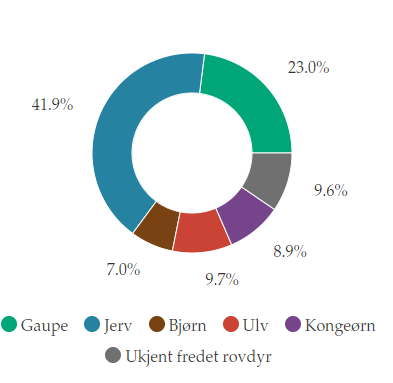
\includegraphics[]{Figurer/diagram/andel_rovvilt_diagram.png}
\caption{Fordeling av fredet rovvilts andel av total tap av sau}
\source{Rovbase \cite{RovbaseErstatningSau}}
\label{fig:rovdyr_andel}
\end{figure}

\noindent
Parallelt som det arbeides med sikre levedyktige rovviltbestander, er det også lagt ned stor innsats for å redusere tap av sau til rovvilt. Det har vist seg å gi en positiv effekt \cite{Klima-ogmiljdepartementet2020RekordlaveRovvilt}. Selv om antall innmeldte tap og påviste rovviltskader har blitt stadig færre, er det et ønske om å redusere tap av sau til rovvilt ytterligere \cite{Miljdirektoratet2020RekordlavtSau}. Dette gjelder særlig i Trøndelag, som er det fylket som stod for størst tap av sau til rovvilt i 2020 \cite{Miljdirektoratet2021Rovvilt2020}. Samme år ble det bevilget omlag 80 millioner kroner til tiltak som rovviltavvisende gjerder, beiteslipp og tidlig nedsanking \cite{Klima-ogmiljdepartementet2020RekordlaveRovvilt}. Andre tiltak som kan bidra til mer effektiv sanking av beitedyr samt bidra til å finne døde eller skadde dyr vil også bli støttes av statlige tilskudd \cite{Klima-ogmiljdepartementet2020RekordlaveRovvilt}. Kostnadene for å dekke erstatning av sau og lam til rovvilt var i 2020 på nærmere 38 millioner kroner \cite{Miljdirektoratet2021Rovvilt2020}. Effektivisering av oppsynsturer vil derfor ikke bare kunne forebygge lidelse blant småfe og gjøre prosessen for oppsyn enklere for bønder og beitelag, men også være økonomisk gunstig for både bønder og staten. 

\section{Involverte myndigheter}
Myndighetene som er involvert i oppfølging av sau på beite i Norge er per dags dato kommunen og Statsforvalteren som er relevant for det respektive beitelaget, samt Mattilsynet og Statens Naturoppsyn. I denne seksjonen skal deres ansvarsområde og informasjonsflyten mellom dem og bøndene beskrives. 

\subsection{Statsforvalteren}
Statsforvalteren (tidligere Fylkesmannen) har ansvar for å følge opp vedtak, mål og retningslinjer fra Stortinget og regjering, og har i tilegg en viktig rolle som bindeledd mellom stat og kommune \cite{Statsforvalteren202HistoriaStatsforvalteren}. I sammenheng med oppfølging av sau på beite, har Statsforvalteren ansvar for forvaltning av  \cite{Statsforvalteren2021Styringsdokumenter}: 
\begin{itemize}
    \item Produksjonstilskudd til beitelag.
    \item Tilskudd til spesielle miljøtiltak i jordbruket (SMIL) som fremmer natur-og kulturverdiene i jordbrukets kulturlandskap og redusere forurensningen fra jordbruket \cite{LandbruksdirektoratetTilskuddSMIL}.
    \item Erstatning for beitedyr tatt av rovvilt.
    \item Tilskudd til forebyggende og konflikt-dempende tiltak.
\end{itemize}

\subsection{Mattilsynet}
Mattilsynet er et statlig forvaltningsorgan med ansvar for å fremme blant annet dyrehelse og etisk forsvarlig hold av dyr \cite{Mattilsynet2021OmMattilsynet}. Dette arbeidet utføres ved å veilede om regelverk, formidle informasjon og føre risikobasert oppsyn for å forebygge dyrelidelser og utbrudd av smittsomme sykdommer \cite{Mattilsynet2021OmMattilsynet, Mattilsynet2021SauGeit}. Mattilsynet får tilsendt beitelagets rapport over oppsynsturene fra Statsforvalteren og gjennomfører en risikovurdering av dyrevelferden på utmarksbeite \cite{Mattilsynet2019TapRovvilt}, mer detaljer om risikoklassene er beskrevet i \ref{dyrevelferd}. Dersom Mattilsynet konkluderer med at dyreeier ikke tilfredsstiller kravene for god dyrevelferd, kan Mattilsynet kreve at dyreeier iverksetter risikoreduserende tiltak som deriblant økt oppsyn \cite{Mattilsynet2019TapRovvilt}. Retter ikke dyreholderen seg etter Mattilsynets pålegg vil Mattilsynet trappe opp bruken av virkemidler, som tvangsmulkt, overtredelsesgebyrer eller å gjennomføre tiltak på eierens regning \cite{Mattilsynet2019TapRovvilt}. I de mest alvorlige tilfellene kan Mattilsynet ta dyrene i midlertidig forvaring eller omplassere dem, avvikle dyreholdet, nekte den ansvarlige å drive aktiviteter som har med dyr å gjøre eller anmelde forholdet til politiet \cite[~s.4]{Mattilsynet2020Mattilsynets2020}. 

\subsection{Statens Naturoppsyn}
\acrfull{sno} er en avdeling i Miljødirektoratet og opererer som miljøforvaltningens operative feltorgan \cite{KjrstadStatensSNO}.
Hvis den oppsynsansvarlige finner et skadd eller dødt dyr og mistenker at det er et fredet rovvilt som står bak, må dyreeieren selv ta kontakt og vise kadaveret til \acrshort{sno} \cite[~s.18]{StatsforvaltereniInnlandet2020InformasjonInnlandet}. \acrshort{sno}s rovviltkontakter vil vurdere kadaveret og konkludere om skaden skyldes rovvilt eller ikke. Alle tap av husdyr erstattes fullt ut etter innsendt søknad hvis det er påvist at fredet rovvilt har forårsaket tapet \cite[~s.18]{StatsforvaltereniInnlandet2020InformasjonInnlandet}. Det gis også erstatning når det er sannsynlighetsovervekt for at tapet skyldes rovvilt \cite[~s.18]{StatsforvaltereniInnlandet2020InformasjonInnlandet}. For å komme frem til en konklusjon om tapet skyldes rovvilt, vil Statsforvalteren bruke opplysningene om beitelagets besetning og drift fra søknaden samt innhente kunnskap om rovviltbestandene og tapsforholdene i området fra kommune/landbrukskontoret og Mattilsynet \cite[~s.18]{StatsforvaltereniInnlandet2020InformasjonInnlandet}.

\begin{figure}[H]
\centering
\captionsetup{width=.8\linewidth}
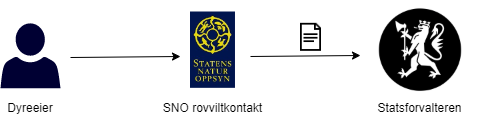
\includegraphics[width=0.9\linewidth]{Figurer/diagram/informasjonsflyt rovvilt.png}
\caption{Informasjonsflyt ved erstatning for sau drept av fredet rovvilt}
\label{fig:informasjonsflyt_rovvilt}
\end{figure}

\subsection{Informasjonsflyt ved innsending av oppsynturrapporter}
Dersom et beitelag ønsker å søke om tilskudd til produksjon og drift av beitelaget, må de lage en samlet rapport over alle oppsynsturene som er gjennomført over perioden der dyrene er på utmarksbeite med nødvendig informasjon \cite{Statsforvalteren2021Styringsdokumenter}. Med nødvendig informasjon menes opplysninger som antall døde og skadde dyr, funn eller observasjoner fra rovvilt, beiteforhold, kartinformasjon der observasjonen fant sted osv. Denne rapporten blir sendt til den aktuelle kommunen. \acrshort{nsg} har lagt ut et forslag til slik rapportskjema på deres nettsider, og dette skjemaet har blitt brukt som utgangspunkt for den innsendte rapporten til Stasforvalteren, se vedlegg \ref{rapportskjema}. Etter at kommunen har godkjent rapporten, blir den sendt videre til Statsforvalteren som har ansvaret for å forvalte produksjonstilskuddet og andre relevante tilskudd. Statsforvalteren videresender også oppsynsrapportene til Mattilsynet, som vil gjennomføre en risikovurdering av dyrenes velferd på beitet. Denne flyten er visualisert i figur \ref{fig:informasjonsflyt_rapport}.

\begin{figure}[H]
\centering
\captionsetup{width=.8\linewidth}
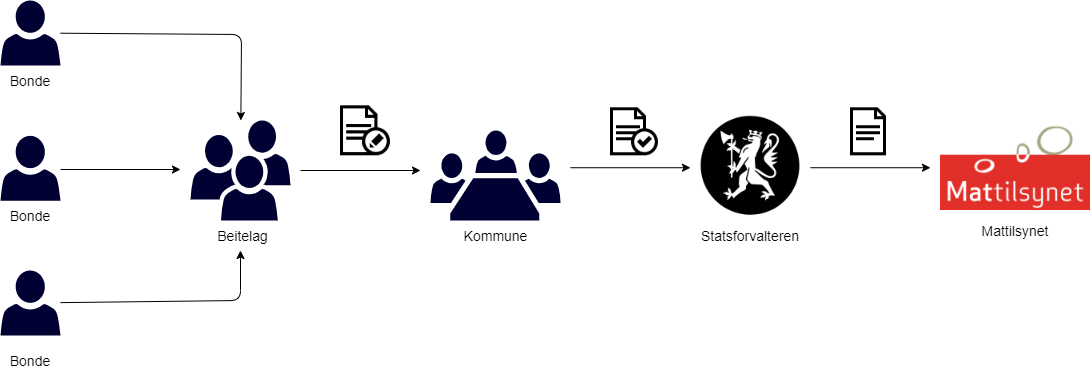
\includegraphics[width=0.9\linewidth]{Figurer/diagram/informasjonsflyt tilsynsrapport.png}
\caption{Informasjonsflyt mellom sauebønder og involverte myndigheter for innsending av oppsynsturrapporter}
\label{fig:informasjonsflyt_rapport}
\end{figure}

\section{Krav fra myndighetene}
\subsection{Oppfølging}
For å beskytte småfe fra unødig lidelse og død, er bønder lovpålagt å føre oppsyn av småfe på utmarksbeite minst én gang i uken \cite{2014ForskriftRovvilt}. I områder med kjent forekomst av rovvilt, må oppsynsfrekvensen være hyppigere enn én gang i uken \cite{2014ForskriftRovvilt}.

\subsection{Øremerking}
Småfe på beitet skal merkes med øremerker som er godkjent av Mattilsynet \cite{2005ForskriftSmafe}. Sau skal merkes med både elektronisk og visuelt merke 30 dager etter fødsel \cite{Mattilsynet2013remerkingSmafe}. Disse elektroniske øremerkene kan deretter leses av med en elektronisk håndleser for å lese av data \cite[~s.48]{BungerSmafenaring2018}. Følgende informasjon skal være med i øremerket for at dyret skal kunne identifiseres \cite{2005ForskriftSmafe}: 
\begin{itemize}
    \item Mattilsynet: MT.
    \item Nasjonalitetsidentifikasjon: NO.
    \item Dyreholdets spesielle identitetsnummer tildelt av Mattilsynet: 7 siffer.
    \item Individnummer: 5 siffer der første siffer er fødselsårets siste siffer og de følgende siffer er dyrets individ nummer.
\end{itemize}
Figuren under viser et eksempel på et øremerke for sau: 

\begin{figure}[H]
\centering
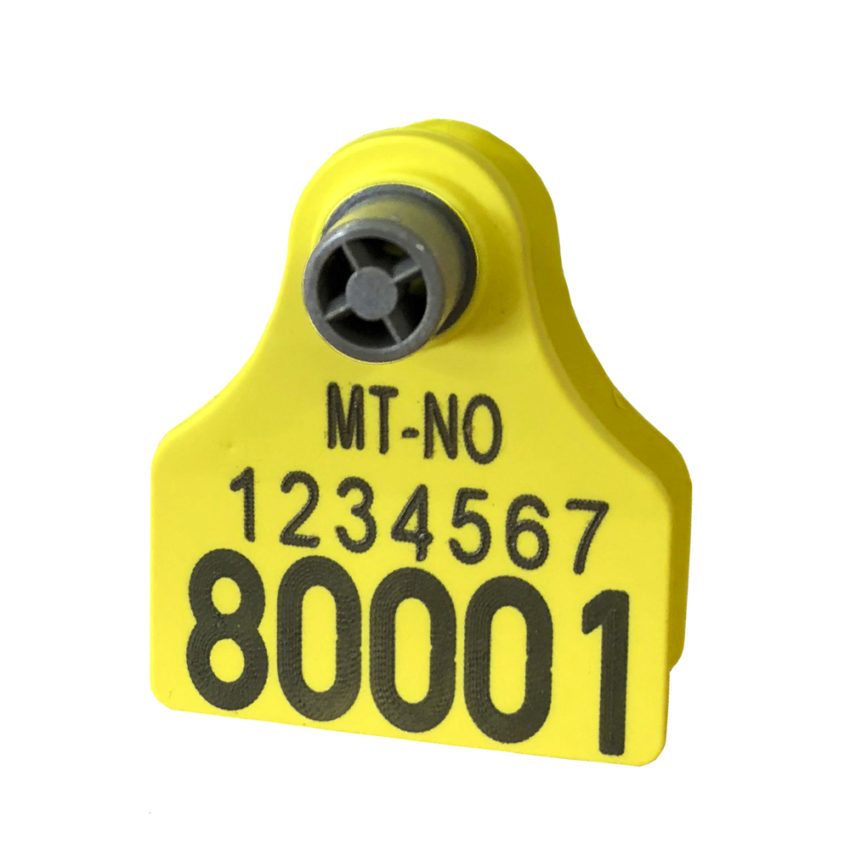
\includegraphics[scale=0.25]{Figurer/Bilder/oremerke.jpg}
\caption{Øremerke for sau}
\source{\cite{OSIDASCombiremerke}}
\label{fig:oremerke}
\end{figure}

\subsection{Dyrevelferd} \label{dyrevelferd}
For å sikre god helse og trivsel blant småfe samt sikre at det tas hensyn til dyrenes naturlige behov, er bønder lovpålagt å holde småfe på egnet utmarksbeite i minst 16 uker hvert år \cite{2005ForskriftSmafe}. Med utmarksbeite menes beite i naturlig vill vegetasjon, skog og fjellterreng som ikke blir kultivert eller gjødslet \cite[~s.55]{BungerSmafenaring2018}. Ansvaret for dyrenes velferd på utmarksbeite ligger hos dyreeier \cite{Mattilsynet2019TapRovvilt}. Mattilsynet vil sørge for at dyreholdet følges i henhold til dyrevelferdsloven; forskriften for velferd hos småfe og produksjonsdyr \cite{Mattilsynet2019TapRovvilt}. Dyreeier og gjetere på oppsynstur har meldeplikt dersom det oppdages smitteutbrudd, rovvilt eller andre årsaker til lidelse eller død blant dyrene på utmarksbeite. Mattilsynet opererer med tre risikoklasser for dyr på utmarksbeite \cite[~s.6]{Mattilsynet2019TapRovvilt}: 

\begin{itemize}
    \item \textbf{Lav risiko}
    \newline
    Tap av under 2\% for søyer, 6\% for lam og 4\% på besetningsnivå ligger innenfor det akseptable, men det forutsettes at det arbeides for å redusere totaltapet på sikt.
    \item \textbf{Middels risiko}
    \newline
    Tap mellom 2-6\% på søyer, 6-15\% på lam og mellom 4–10\% på besetningsnivå ligger innenfor et område hvor det forventes at forebyggende tiltak planlegges og gjennomføres.
    \item \textbf{Høy risiko}
    \newline
    Tap over 6\% på søyer, 15\% på lam og 10\% på besetningsnivå er i utgangspunktet uakseptabelt dyrevelferdsmessig sett. Forebyggende tiltak må planlegges og gjennomføres. 
\end{itemize}

\noindent
Mattilsynet vil vurdere risikonivået for hver enkelt beitelag ut i fra lokal kunnskap om beiteforholdene fra regionale representanter fra \acrlong{obb}, \acrfull{nibio} og søknadene for produksjonstilskudd og erstatning for tap av sau på beite \cite{Mattilsynet2019TapRovvilt}. Oversikt over estimert rovviltbestand og dokumenterte tap til rovvilt blir også hentet fra Rovbase \cite{Mattilsynet2019TapRovvilt}. 

\section{Gjennomføring av oppsyn}
I dag er det vanlig at flere bønder fra nærliggende områder går sammen og oppretter et beitelag der de samarbeider om oppsyn, sanking eller andre aktiviteter knyttet til utmarksbeite \cite[~s.57]{BungerSmafenaring2018}. I 2017 var ca. 74\% av all sau som ble sluppet på utmarksbeite inkludert i et organisert beitelag \cite{NorskSauogGeit2018OrganisertBeitebruk}. Beitelag er et av tiltakene i ordningen kalt \acrfull{obb} som ble opprettet i 1970 som et samarbeid mellom Landbruksdepartementet og \acrfull{nsg} \cite{NorskSauogGeit2018OrganisertBeitebruk}. Hovedmålsettingen for \acrshort{obb} er å legge til rette for en mer rasjonell utnytting av utmarksbeitene og redusere tapet av dyr på beite til et minimum \cite{NorskSauogGeit2018OrganisertBeitebruk}. I 2003 ble innført krav der beitelag må registreres i enhetsregisteret i Brønnøysund for å være berettiget tilskudd \cite{NorskSauogGeit2018OrganisertBeitebruk}.

\subsection{Før utslipp}
\acrshort{nsg} har kommet ut med en offisiell anbefaling om at søyer som skal slippes løs på utmarksbeite bør merkes med bjelleslips \cite{NorskSauogGeitBjelleslips}. Et bjelleslips er et merke som indikerer antall lam som er tilknyttet en søye med fargekoder, se figur \ref{fig:bjelleslips} under. Det gjør det mulig å for personer på oppsynsturer å få oversikt over dyretall på utmarksbeite. Det kan også lønne seg med bjelleslips dersom ens saueflokk blander seg med en annen besetning som ikke benytter seg av bjelleslips \cite[~s.27]{FylkesmanneniOsloogAkershus2017BeitedyrRovdyr}. 

\begin{figure}[H]
\centering
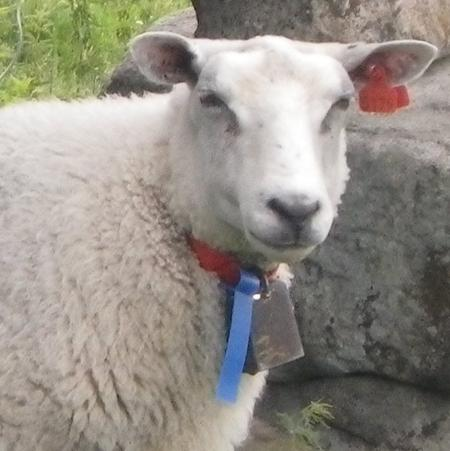
\includegraphics[scale=0.3]{Figurer/Bilder/bjelleslips.jpg}
\caption{Bjelleslips for sau}
\source{\cite{NorskSauogGeitBjelleslips}}
\label{fig:bjelleslips}
\end{figure}

\noindent
\acrshort{nsg} anbefaler å bruke samme fargekoding for slips som for fostertelling, som er når man undersøker antall fostre i en drektig søye med ultralyd \cite{FostertellingOgSniktitt2015}. Fargekodingen kan variere fra landsdel til landsdel. Masteroppgaven vil ta utgangspunkt i fargekodene som brukes i Oppdalområdet etter professor Hvasshovds erfaring med Søndre Trollheimen Beitelag som er følgende: 
\begin{itemize}
    \item Blått slips: 0 lam. 
    \item Grønt slips: 1 lam.
    \item Gult slips: 2 lam.
    \item Rødt slips: 3 lam. 
\end{itemize}
Det er ikke alle bønder som markerer at en søye ikke har lam og vil da bare unnlate å markere søyen med bjelleslips.

\subsection{På utmarksbeite}
Det er ikke en fastsatt dato for når småfe blir sluppet til utmarksbeite, men det skjer som oftest kort tid etter lammesesongen som forekommer rundt april og mai \cite{yrehagen2015BeiteUtmark}. Dyrevelferdsloven krever at samtlige dyr har god helsetilstand og at lam er sammen med mordyr og i stand til å holde følge med mora på beitet \cite{2005ForskriftSmafe}. Dyreeier må derfor selv vurdere hva som er best slippetidspunkt for sine dyr ut i fra deres alder og tilstand, og forholdene på beiteområdet \cite{NorskSauogGeitRiktigSlippetidspunkt}. Slipptidspunktet må være sent nok til det er nok beite som gir god nok næring slik at lammene får en jevn og god tilvekst, men tidlig nok til at søyene kan sortere ut de gode beiteplantene mens de er unge og næringsrike \cite[~s.8]{RekdalTemahefteSau}. Hvis beiteområde inneholder for eksempel høy vannføring i bekker, snøfonner o.l, må lammene være tilsvarende robuste \cite{NorskSauogGeitRiktigSlippetidspunkt}. 
\newline
\newline
Selve gjennomføringen av oppsynsturene vil naturlig nok variere fra bonde til bonde. Turene kan gjennomføres enten av den enkelte bonde eller gjennom organiserte beitelag. Heretter vil personer som utfører oppsynsturer bli referert til som oppsynsansvarlig. Per i dag utføres oppsynsturer ved at den oppsynsansvarlige, enten manuelt eller ved hjelp av digitale verktøy (eksempler på slike verktøy presenteres i kapt. \ref{sporing}), først sporer opp dyreflokken. Ettersom dyrene beveger seg raskt over store områder og gjerne i ulendt terreng, må den tilsynsansvarlige som regel observere dyrene på avstand med kikkert og deretter notere informasjon som antall og tilstand med penn og papir. Å registrere riktig antall kan fort bli en utfordring siden sauene gjerne beveger seg mens den tilsynsansvarlige ser vekk ifra kikkerten for å notere. De store avstandene fører også til at det kan være vanskelig å få øye på øremerker eller bjelleslips, selv med kikkert. I tillegg til antall sauer på beitet, vil dato, rute for oppsynstur og opplysninger som skadde dyr, årsak, observasjon av rovvilt og beiteforhold bli registrert. Ifølge professor Hvasshovds erfaring med tilsynsturer, pleier det å ta ca. 2-3 timer, men det kan ta opptil 10 timer dersom det er vanskelig å spore opp hele dyreflokken. 

\subsection{Sanking}
I følge \textit{Forskrift om velferd for småfe} \S 27 så har dyreeier ansvar for at småfe på utmarksbeite hentes hjem i god tid før det ventes frost eller snøfall om høsten \cite{2005ForskriftSmafe}. I følge data fra \acrlong{obb} pleier nedsankingen av sau å foregå i september \cite[~s.8]{Stornes2017TidligInnmarksbeite}. Tidlig innsanking av dyrene i august kan forekomme som et tiltak for å forebygge tap av småfe til rovvilt, da særlig jerv. Over 80 \% av skader på sau og lam utført av jerv blir påvist etter 1.august, og nesten halvparten av disse skjer etter 1.september \cite{Messel2016BondeMedisin}. Dersom en sauebonde velger å gjennomføre tidlig innsanking av dyrene, skal bonden bli kompensert for økningen av kostnadene for kraft -og grovfôr som følge av at dyrene må flyttes til innmarksbeite \cite[~s.10]{Stornes2017TidligInnmarksbeite}. Selve nedsanking av sau er utfordrende, ettersom det kan være vanskelig å finne hele dyreflokken og det er store områder å dekke. Hvis et beitelag har sluppet dyrene samlet, må dyrene også sorteres etter nedsankingen slik at dyrene drar til riktig bonde \cite{NorturaMedlem2016UtformingSA}. 

\section{Konklusjon}
Det er lovpålagt for norske sauebønder å slippe sau på utmarksbeite i minst 16 uker årlig. Hvert år mister 3-7\% av sauer sluppet på utmarksbeite livet grunnet sykdom, ulykker eller rovdyr. Selv om tallene på tap av sau på beite er i nedgående trend, arbeides det med å senke tapene ytterligere både for å minimere dyrenes lidelser samt de økonomiske tapene det forårsaker. Dette arbeides med både fra sauebøndene og beitelagenes side, og fra offisielle myndigheter som Statsforvalteren, Mattilsynet og Statens Naturoppsynet. Et av tiltakene for å redusere tap er å utføre ukentlige tilsynsturer der dyreflokkens antall og tilstand sjekkes, samt om det rovvilt tilstede i nærområdet. Oppsynet gjennomføres ved at den personen som er ansvarlig for tilsyn sporer opp dyreflokken og registrerer relevant informasjon som videresendes til Statsforvalteren og Mattilsynet, som vil vurdere om det er behov for ytterligere tiltak for å sikre velferden til dyrene eller gi erstatning for tapte dyr. 
\chapter{Inspirasjon og tidligere arbeid}
I dette kapittelet vil eksisterende digitale løsninger som brukes i sammenhenger relevant til sporing og registrering av sau undersøkes og vurderes. Avslutningsvis vil arbeidet og resultatet fra fordypningsprosjektet bli presentert, som masteroppgaven har lagt til grunne og bygd videre på.  

\section{Eksisterende løsninger}
I dag finnes det ulike digitale løsninger som forenkler prosessen med tilsynstur på utmarksbeitet. Disse løsningene gjør en av to ting; enten bytter ut dagens system med sporingsbrikker eller et nytt digitalt system for manuell registrering av dyr på utmarksbeite. Slike løsninger skal vi presentere og undersøke i dette kapittelet. 

\subsection{Elektronisk sporing av dyr} \label{sporing}
 Utviklingen av teknologi knyttet til småfehold har utviklet seg raskt de siste ti årene for å gjøre det enklere for bonden å ha kontroll på småfeet på beite \cite[~s.49-50]{BungerSmafenaring2018}. For teknologi brukt utendørs, er automatisk sporing av dyrene med såkalte radiobjeller mest brukt blant bønder \cite[~s.50]{BungerSmafenaring2018}. Slike radiobjeller plasseres rundt halsen på sauen når den er på beite og gir signaler om dyrenes lokasjon til bonden ved hjelp av \acrshort{gps} eller mobilnettet \cite{Fremstad2020SauebnderRuralis}. De største aktørene i det norske markedet for radiobjeller er Telespor \cite{Telespora} og Findmy. De seneste årene har disse aktørene har fått konkurranse fra nye aktører som blant annet Smartbjella \cite{SmartbjellaSporing}.  
 
 \begin{figure}[H]
\centering
\captionsetup{width=.8\linewidth}
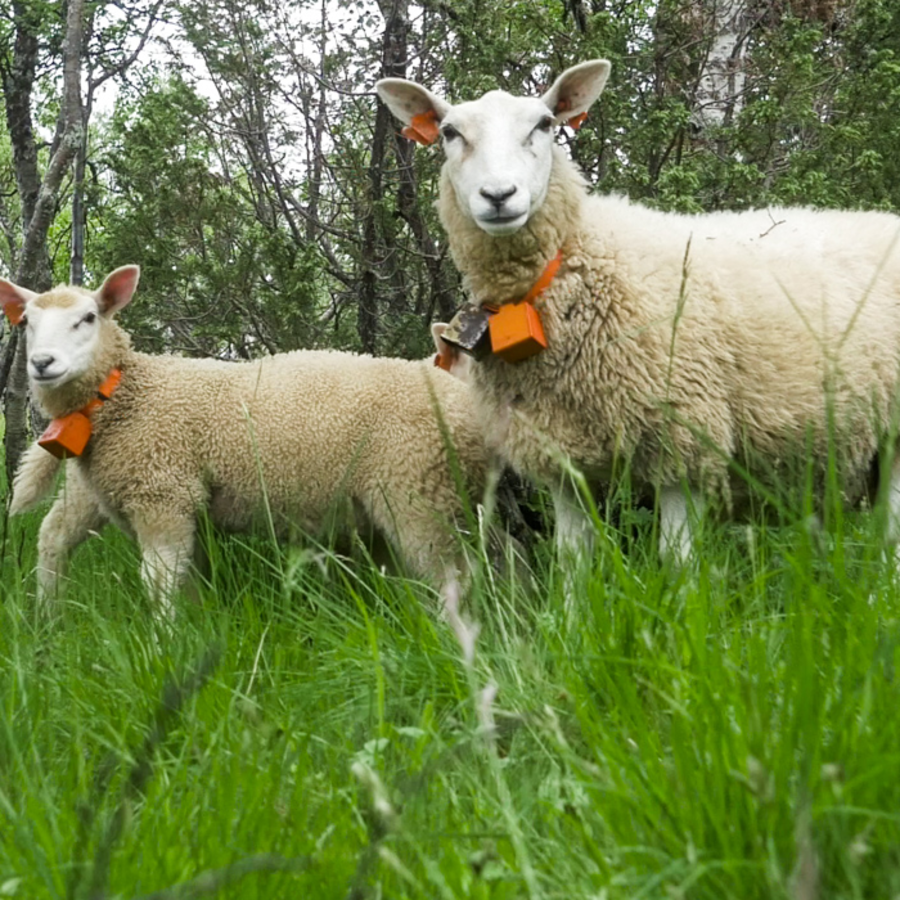
\includegraphics[scale=0.3]{Figurer/Bilder/findmy_bjeller.png}
\caption{Sauer utstyrt med radiobjeller fra FindMy}
\source{\cite{findmyProdukt}}
\label{fig:radiobjeller}
\end{figure}
 
 \subsubsection{Telespor}
 Telespor har vært på markedet siden 2004 med elektronisk sporing av husdyr på beite over lengre tid med "Radiobjella" som benytter seg av GPS lokalisering, og har lansert sin fjerde generasjons radiobjelle \cite[~s.69]{kvamRoleAdvisoryServices2019} \cite{ProduktTelespor}. Tidligere generasjoner av radiobjella brukte \acrshort{gsm}/\acrshort{gprs}, det vil si 2G mobilnettet, for å motta GPS posisjon fra satellitter til Telespors server som deretter videresendte informasjonen til kundens brukerportal  \cite{Telesporsystemet}. Dagens fjerde generasjons radiobjelle benytter seg av nyere \acrfull{nbiot} og \acrshort{lte}, som muliggjør at sensorer og andre enheter kan kommunisere med 4G-nettet raskere og med svært lav energibruk \cite{lorentzenTingenesInternettInntar2018, ProduktTelespor}. Telespor bruker Telenors IoT-dekning på 4G-nettet. Dette gjør at radiobjellene er avhengig av at det er dekning i området for å kunne kommunisere med bonden. Radiobjellene er også utstyr med bevegelsessensorer som kan utløse tre alarmer \cite{ProduktTelespor} dersom: 
 \begin{itemize}
     \item Dyret har ikke beveget seg de siste 3 timene.
     \item Dyret har vært på samme posisjon i en lengre periode.
     \item Radiobjella har ikke klart å sende sin posisjon de siste 2 rapportene
 \end{itemize}
 \noindent
Sendeintervall og alarmsensitivitet kan endres på når som helst av brukeren \cite{ProduktTelespor}. Selve bjellene er utstyrt med utskiftbare batteri som det anbefales at man skifter etter hver sesong \cite{ProduktTelespor}. Telespor bruker en betalingsmodell der brukere må betale en sum for radiobjellene og et sesongbasert abonnement som dekker både mobildatatrafikken, tilgang til brukerportalen og et batteri \cite{telenorDekningIoTPa, TelesporNettbutikka}. Per dags dato er prisen på en fjerde generasjons radiobjelle 1124 kr og sesongabonnement 124 kr \cite{TelesporNettbutikka}.

\subsubsection{FindMy}
FindMy, tidligere kalt FindMySheep, ble skapt av sauebønder i 2009 som ønsket elektronisk sporingsutstyr som ikke var avhengig av mobilnettet \cite{findmyOmOss}. FindMys e-bjeller er bygd rundt lavbane satellitt teknologi og er dermed ikke avhengig av verken \acrshort{gsm} eller \acrshort{nbiot} for å fungere og vil i praksis fungere over hele verden \cite{findmySatelitt}. Det vil si at e-bjella har dekning så lenge den har fri sikt til himmelen. E-bjella har også en funksjon der den vil prøve å sende signaler flere ganger for å få tilfredstillende resultat dersom e-bjella er i et område med utfordrende terreng og topografi \cite{findmyDekningHeleNorge}. Alle e-bjellene kan settes opp med egendefinerte meldingsplaner som bestemmer hvor ofte man får oppdateringer om dyrets posisjon i løpet av en dag \cite{findmySlikFungererSatellittene}. I tillegg til elektronisk sporing har e-bjella Model 2 funksjoner som sporingsdata og tilvekstkart fra Sauekontrollen, søk med Bluetooth, geofencing, urovarsel som detekterer unormal adferd i flokken og sporlogg som samler posisjoner e-bjella har sendt i en valgt periode for å gi innsikt beitemønster \cite{findmyFunksjoner}. FindMy anbefaler selv at man sporer minst 25\% av dyreflokken for å få god oversikt over dyrene \cite{findmyProdukt}. Ca. 40 000 e-bjeller fra FindMy er i bruk per dags dato \cite{findmyFunksjoner}. Per i dag koster én enkelt e-bjelle 1849 kr, og årlig brukeravgift kommer på 229 kr per bjelle \cite{findmyShop}. Lik som Telespor har også e-bjella til FindMy utskiftbarebatteri, men disse skal vare 2-3 beitesesonger og koster 99 kr per stykk \cite{findmyBrukeravgift}. 

\subsubsection{Smartbjella}
Smartbjella/Smartbells ble lansert i 2019 etter at ansatte ved morselskapet StalkIT \cite{HomeStalkITNo} oppdaget at deres teknologi for å spore opp konteinere kunne være nyttig for å spore sauer på beite \cite{SMARTBELLSEmisjonskampanjeFolkeinvest2019}. Smartbjella var den første aktøren som benyttet seg av IoT-teknologi innenfor dyresporing, etter å ha inngått avtaler med Telenor og Telia om å bruke deres \acrshort{nbiot} nettverk  \cite{henriksenKonkurransenBeitetechHardner2020}. Det benyttes også \acrshort{gnss} for nøyaktig posisjonering \cite{PRODUKTSmartbjellaSporing}.  Smartbjella nyeste versjon 2 som er ute for pre-salg i 2021 inkluderer dødsalarm, frekvensstyring av signalene fra bjellen, historisk bevegelsesmønster, temperaturmåler, Bluetooth og mulighet til å sette opp geofence \cite{PRODUKTSmartbjellaSporing}. Smartbjella skal være vedlikeholdfri per sesong \cite{PRODUKTSmartbjellaSporing}. Ved normale værforhold og med et rapporteringsintervall på 24 timer skal batteriet i Smartbjella holde opptil 15 år. \cite{PRODUKTSmartbjellaSporing}. Prisen for Smartbjella 2 ligger på 949 kr per enhet og abonnement på en sesongbruk av smartbjella ligger på 100 kr per enhet \cite{SmartbjellaPresalg2021}. Det er også mulig å leie radiobjeller \cite{SMARTBELLSEmisjonskampanjeFolkeinvest2019}. Per dags dato er det 18000 radiobjeller fra Smartbjella i Norge \cite{SmartbjellaSporing}. 

\subsubsection{Konklusjon/Evaluering}
Alle bedriftene som er nevnt i forrige delkapittel er i markedet for elektronisk sporing av dyr på utmarksbeite og arbeider med å gjøre det lettere for bønder å lokalisere dyreflokken og få tilbakemeldinger om dyrenes tilstand. Teknologiene som utnyttes for elektronisk sporing er relativt like, spesielt etter at Telespor også byttet over til å bruke \acrshort{nbiot} og \acrshort{lte}, med unntak av FindMy som benytter seg av lavbane satellitter. Dette er en fordel her i Norge, der dyrene ofte ferdes på øde steder uten mobildekning på utmarksbeite. Alle aktørene tilbyr også en form for alarmfunksjonalitet som gir tilbakemelding dersom et dyr har vært inaktiv over en periode. Betalingsmodellene er også tilnærmet identiske, med en pris for selve radiobjellene og brukeravgift/abonnement på servicetjenester, samt tilleggskostnader for batteri som eventuelt må skiftes ut. Her skiller Smartbjella seg ut ved at batteriene har mye lengre levetid. Smartbjella gir mer fleksibilitet da det er mulig å bare leie bjellene ved behov ønskelig \cite{SMARTBELLSEmisjonskampanjeFolkeinvest2019}. Prismessig ligger Telespor og FindMy på rundt 1500-2000 kr for en hel pakke inkludert bjelle og brukeravgift, mens Smartbjella er rimeligere med enheter og brukeravgift på rundt 1000 kr. 
\newline 
\newline
Store kostnader knyttet til utstyr og vedlikehold er nettopp en av grunnen til at mange bønder tidligere ikke ønsket å benytte seg av radiobjeller, men de siste årene med nyere, mer stabil teknologi og konkurranse fra flere aktører på markedet som presser prisene ned, er det nå flere og flere bønder som prøver ut  radiobjeller. I rovdyrutsatte områder kan også beitelag søke om tilskudd til konfliktdempende tiltak som deriblant elektronisk overvåkningsutstyr, der Statsforvalteren kan dekke deler av kostnadene for slik investering Dette har gjort at flere bønder fikk testet radiobjeller og senere begynt å benytte seg av det \cite[~s.61, 66]{kvamRoleAdvisoryServices2019} \cite{landbruksdirektoratetTilskuddTilTiltak}.  
\newline
\newline
I 2009 - 2012 ble det utført et nasjonalt beiteprosjekt på vegne av Statens landbruksforvaltning (nå Landsbruksdirektoratet) med formål å få bedre sauehold med mindre tap av dyr på beite \cite{statenslandbruksforvaltningNasjonaltBeiteprosjekt20092013}. Utprøvingen av  radiobjeller ble evaluert av \acrfull{tfou} \cite[~s.8]{statenslandbruksforvaltningNasjonaltBeiteprosjekt20092013}. Rapporten konkluderte med at det antakelig er en forebyggende tapsreduserende effekt med bruk av radiobjeller og at det førte til bedre dyrevelferd ettersom bjellene ga raskere avdekking av unormal adferd blant dyrene samt mer effektiv sanking på høsten \cite[~s.40]{statenslandbruksforvaltningNasjonaltBeiteprosjekt20092013}. Bøndene selv rapporterte økt produktivitet fordi radiobjellene gjorde arbeidet om å lokalisere dyrene i sammenheng med tilsyn og sanking lettere, som igjen førte til høyere tilfredshet blant bøndene og økt motivasjon til å bruke utmarksbeite \cite[~s.41]{statenslandbruksforvaltningNasjonaltBeiteprosjekt20092013}, \cite[~s.60]{kvamRoleAdvisoryServices2019}. Tapte dyr med radiobjeller hadde økt gjenfinningsrate og bedre mulighet til å fastslå dødsårsak enn dyr uten radiobjeller \cite[~s.40]{statenslandbruksforvaltningNasjonaltBeiteprosjekt20092013}. 
\newline
\newline
Selv om overvåkningsteknologien for dyr på utmarksbeite stadig forbedres og prisen for utstyret senkes, er det fortsatt ikke vanlig å sette radiobjeller på alle dyrene. Elektronisk sporing av dyr erstatter ikke oppsynsturer som bøndene fortstatt er lovpålagt å dra til beitet for å sjekke dyrenes tilstand, men det er et nyttig verktøy som gjør dette arbeidet lettere å gjennomføre.

\subsection{Registrering av dyr i utmark} 
Per dags dato er det ingen aktive applikasjoner som legger til rette for registrering av dyr i utmark, men det finnes løsninger som har vært innom denne ideen tidligere. Beitesnap var en applikasjon som tok for seg registrering av tilsyn for husdyr på beite, både for bønder under beitesesongen og for privatpersoner som ønsker å melde fra om beitedyrsobservasjoner \cite{BeitesnapRevolusjonerendeVerktoy}. I tillegg er det gjennomført tidligere masteroppgaver med lignende problemstilling, som for eksempel applikasjonen Lambo som ble utviklet for oppgaven \textit{Effektivisering av manuell oppfølging av sau på utmarksbeite} fra 2018 \cite{dystheEffektiviseringAvManuell2018}. Det er også flere pågående masteroppgaver per våren 2021 som utforsker samme tema som denne masteroppgaven.  

\subsubsection{Beitesnap}
Beitesnap av Fant AS er en applikasjon som ble lansert i 2017 som et verktøy for å registrere observasjoner av husdyr på beite \cite{BeitesnapRevolusjonerendeVerktoy}. Applikasjonen avsluttet driften fra og med 2020 grunnet dårlig økonomi som følge av få brukere \cite{BeiteSnapFacebook2020}. Applikasjonens målgrupper var beitebrukere som kunne legge inn sitt beiteområde og dyrenes individnummer slik at de kan få meldinger fra andre som observerer skadde eller døde dyr innenfor bondens beiteområde \cite{BeitesnapRevolusjonerendeVerktoy}. Alle registreringene fra beitesesongen ble samlet og utformet til en rapport som kunne sendes inn til myndighetene \cite{BeitesnapRevolusjonerendeVerktoy}. Beitesnap var også koblet opp mot Norgeskart \cite{NorgeskartKartverketNo}, slik at det var mulig å spore oppsynsturene med \acrshort{gps} \cite{BeiteSnapFacebook2020}. Kartet kunne lastes ned på forhånd for offline bruk \cite{BeitesnapRevolusjonerendeVerktoy}. For å få tilgang til en Beitebruker-konto på Beitesnap, var det en årlig avgift på 1200 kr + MVA \cite{BeitesnapRevolusjonerendeVerktoy}. Privatpersoner som ønsket å sende inn sine observasjonen kunne opprette en gratis bruker, som hadde mulighet til å sende inn bilder med informasjon om dyr de møter på i utmarka \cite{BeitesnapRevolusjonerendeVerktoy}. Dersom observasjonen er innenfor et registrert beiteområdet, vil den aktuelle bonden få beskjed om det \cite{BeitesnapRevolusjonerendeVerktoy}. 
\newline
\newline
Beitesnap har mye lik funksjonalitet som Sauron, men hvordan informasjonen registreres er nokså ulik. I Beitesnap registreres et bilde av observasjonen, hvilket dyreslag som er registrert, om dyret var sett, skadd eller dødt og eventuelt individnummeret til dyret \cite{beitesnapKomplettBrukermanualBeitebrukere2017}. All annen informasjon, som totalt antall dyr, antall søyer og lam, farge på dyrene, øremerker eller bjelleslips må dermed skrives i fritekst. Å observere dyrene på lang avstand for å så måtte taste inn all informasjonen kan være utfordrende, samtidig som det gjør at innrapporteringene er mindre strukturerte. (Prisen for å ha en beitebruker-konto virker også nokså stiv for sauebønder som allerede betaler mye penger for å bruk av elektronisk sporingsutstyr). 

\begin{figure}[H]
\centering
\captionsetup{width=.8\linewidth}
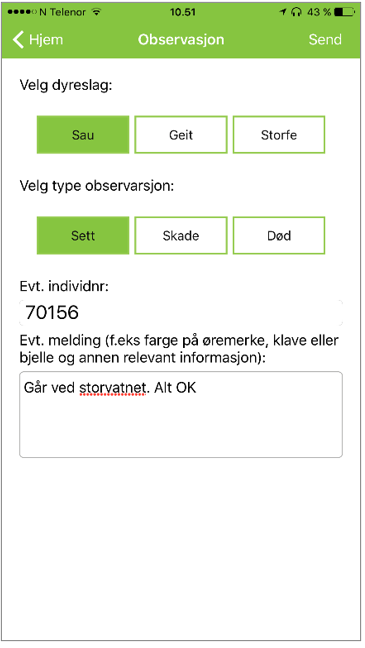
\includegraphics[scale=0.7]{Figurer/Bilder/beitesnap.png}
\caption{Skjermbilde av Beitesnaps registreringsside}
\source{\cite{beitesnapKomplettBrukermanualBeitebrukere2017}}
\label{fig:beitesnap}
\end{figure}

\subsubsection{Tidligere og pågående masteroppgaver}
Det er flere gjennomførte og pågående masteroppgaver fra NTNU som har arbeidet med å effektivisere oppsyn av sauer på utmarksbeite. Denne masteroppgaven har tatt inspirasjon fra masteroppgaven \textit{Effektivisering av manuell oppfølging av sau på utmarksbeite} \cite{dystheEffektiviseringAvManuell2018} skrevet av Stian Dysthe og Andreas Kjerstad der professor Hvasshovd også var veileder. Deres mål for prosjektet var:
\newline
\newline
\textit{Utvikle et produkt som gjør det lett og effektivt å registrere detaljert, strukturert, lokasjonsbasert informasjon om sau på beite, samtidig som det møter behovet til bøndene og krav fra myndighetene} \cite[~s.13]{dystheEffektiviseringAvManuell2018}.
\newline
\newline
I den sammenhengen utviklet de applikasjonen Lambo, som har en del fellestrekk med både Beitesnap og Sauron. Lambo har funksjonalitet som online og offline kart med GPS-sporing av brukerens rute og registrering av observasjoner av både husdyr og rovdyr \cite{dystheEffektiviseringAvManuell2018}. I motsetning til Beitesnap, har Lambo en mer detaljert innrapportering av observasjoner, der brukeren må gå gjennom et registreringsskjema som brukeren må trykke gjennom for å registrere en observasjon istedetfor å skrive det inn som fritekst. Brukeren vil først bli spurt om observasjonen gjelder sau, skadet sau, død sau, ullfunn, hund, rovdyr, reinsdyr eller annet, og deretter få spørsmål om relevante underkategorier som antall, farge osv \cite[~s.84-85]{dystheEffektiviseringAvManuell2018}. Måten å registrere informasjon er det som vil skille Sauron fra Lambo, ettersom denne masteroppgaven vil ha et særskilt fokus på hvordan å registrere observasjonene uten å se på mobilskjermen.

\begin{figure}[H]
\centering
\captionsetup{width=.8\linewidth}
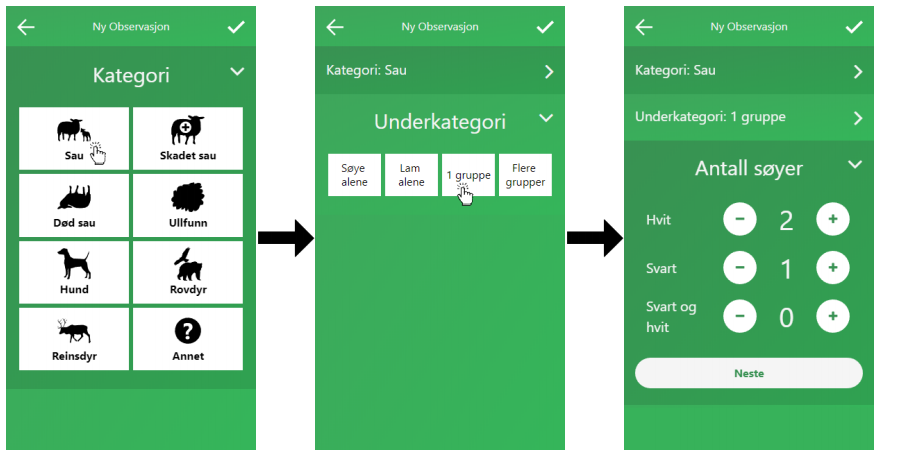
\includegraphics[scale=0.5]{Figurer/Bilder/lambo.png}
\caption{Skjermbilde fra Lambos registreringsskjema}
\source{\cite{dystheEffektiviseringAvManuell2018}}
\label{fig:lambo}
\end{figure}
 
\section{Fordypningsprosjekt}
Denne masteroppgaven bygger videre på arbeidet gjort under fordypningsprosjektet "Tilsyn med Sau På Beite" \cite{Abtahi2020TilsynBeite} som ble gjennomført høsten 2021. Mens denne masteroppgaven går ut på å utvikle et helhetlig produkt for å bistå gjetere på oppsynstur, fokuserte fordypningsprosjektet spesifikt på selve registreringen av sau. Målet med fordypningsprosjektet var: 
\newline
\newline
\textit{Designe og utvikle en applikasjon som muliggjør effektiv registrering av sauer på utmarksbeite i situasjoner der brukeren kontinuerlig benytter seg av kikkert og dermed ikke kan se på skjermen.} \cite[~s. 3]{Abtahi2020TilsynBeite}
\newline
\newline
Denne problemstillingen ble løst ved å først undersøke brukergrensesnitt for skjermer som var utviklet med tanke på bruk i blinde. Det ble så valgt tre ulike brukergrensesnitt, en med Sveiping, en med knapper og en med en kombinasjon av de tidligere to grensesnittene som det ble utviklet prototyper for. Alle brukergrensesnittene benyttet seg av tekst-til-tale for å gi informasjon om registreringen til brukeren mens registreringen pågikk. Deretter ble det utformet og gjennomført ni brukertester som undersøkte feilraten ved registrering, effektiviteten ved kortest gjennomføringstid og hva som var den beste måten å gi tilbakemelding på når skjermen var utilgjengelig. Både de kvantitative og kvalitative resultatene fra brukertestene tilsa at grensesnittet som benyttet seg av Sveiping fungerte best for formålet. Dette resultatet har blitt tatt videre i masteroppgaven, og det er begrunnelsen for at det blir brukt en kombinasjon av sveiping og tapping i brukergrensesnittet for registrering av sau i Sauron.

\section{Konklusjon}
Det brukes stadig mer og mer digital teknologi for å assistere bønder i deres arbeid med å slippe dyr på utmarksbeite. Et av de mer brukte digitale verktøyene som bistår i oppsynsturer er digitale sporingsutstyr som radiobjeller som settes på dyrene og sporer deres lokasjon med GPS-teknologi eller \cite{nbiot}. Per i dag er det minst 3 aktører i Norge som driver radiobjeller; Telespor, FindMy og Smartbjella. Disse aktørene benytter seg av GPS-teknologi som enten \acrshort{nbiot}-nettet eller lavbane satellitt teknologi for sporing, og har i tillegg andre funksjoner som blant annet dødsalarm, tilpasning av innrapportering og geofencing. Tidligere prosjekter som har evaluert bruken av elektronisk overvåkning av dyr på utmarkbeite har konkludert med at radiobjellene kan forebygge tap på beitet ved at farlige situasjoner raskere blir avdekket og samtidig fører til mer effektiv sanking av dyrene på høsten. Likevel vil ikke radiobjeller erstatte manuelle oppsynsturer med det første ettersom norske myndigheter krevet at oppsynsturer skal bli utført ukentlig. Applikasjoner som Beitesnap og Lambo, som ble også utviklet i en masteroppgave, har blitt brukt som inspirasjon. Det ble konkludert at disse applikasjonene manglet funksjonalitet som muliggjør registrering av sau uten å se på mobilskjermen. Hvordan å utføre handlinger på best mulig måte uten å se på skjermen ble undersøkt i fordypningsprosjektet. Under fordypningsprosjektet ble det utformet tre ulike brukergrensesnitt som deretter ble brukertestet. Resultatene fra testene viste at en kombinasjon av sveiping og tapping fungerte best for registrering av sau og dette brukergrensesnittet er brukt som utgangspunkt i masteroppgaven. 
\part{Eget bidrag}

\chapter{Konsept}

\chapter{Kravspesifikasjon}
Dette kapitlet tar for seg kravene som ble utviklet sammen med fungerende produkteier Professor Hvasshovd før og under utviklingen av applikasjonen. Kravene er delt i to i form av funksjonelle krav og ikke-funksjonelle krav. Både de funksjonelle og de ikke-funksjonelle kravene er nummerert og organisert inn i undergrupper. Hvert krav har også en prioritet som forteller hvor viktig det har vært å få implementert det spesifikke kravet. Krav som var absolutt nødvendige for at applikasjonen skulle regnes som ferdig ble merket med prioriteringen \enquote{Høy}. Krav som ikke nødvendigvis måtte implementeres for at applikasjonen skulle regnes som ferdig, men som ville gjøre applikasjonen betydelig bedre er merket med prioriteringen \enquote{Middels}. Til sist er krav som ikke er nødvendig for applikasjonen i det hele tatt, men som ville vært fint å ha med, merket med prioriteringen \enquote{Lav}.

\section{Funksjonelle krav} \label{sec:funksjonelle-krav}
Tabell \ref{tbl:funksjonelle-krav} viser alle de funksjonelle kravene som har blitt utviklet i løpet av prosjektet. Med funksjonelle krav menes krav stilt til funksjonaliteten brukeren skal ha tilgang til under bruk av applikasjonen.
\begin{table}[H]
    \centering 
    \begin{tabular}{| p{0.1\linewidth} | p{0.7\linewidth} | p{0.1\linewidth} |}
       \hline
        Nr. & Beskrivelse & Prioritet \\
        \hline \hline
        F1 & Brukeren skal ha tilgang til de mest oppdaterte kartbildene, som skal løses ved hjelp av Karverkets tjenester (NorgesKart). & Høy \\ 
        \hline
        F1.1 & Brukeren skal kunne laste ned et utsnitt av kartet til offline bruk. & Høy \\ 
        \hline
        F1.2 & Ved bruk av kart skal brukeren kunne se sin posisjon, samt en linje over kartlagte bevegelser. & Høy \\
        \hline
        F1.3 & Brukeren skal kunne legge til observasjoner på kartet i form av pins. & Middels \\
        \hline
        F2 & Brukeren skal kunne registrere en ny oppsynstur. & Høy \\ 
        \hline
        F2.1 & Brukeren skal kunne ha mulighet til å fylle ut nødvendig informasjon om en oppsynstur. & Høy \\ 
        \hline
        F2.3 & Brukeren skal kunne registrere saueflokker på beitet med informasjon som gjør det mulig å kjenne igjen den spesifikke saueflokken ved et senere tidspunkt. & Høy \\
        \hline
        F2.3.1 & Brukeren skal kunne registrere totalt antall sau i en flokk. & Høy \\
        \hline
        F2.3.2 & Brukeren skal kunne registrere antall av hver farge på sauene i flokken. & Høy \\
        \hline
        F2.3.3 & Brukeren skal kunne registrere antall søyer og lam i flokken. & Høy \\
        \hline
        F2.3.4 & Brukeren skal kunne registrere antall av søyer med slips og farge på slipset. & Høy \\
        \hline    
        F2.3.5 & Brukeren skal kunne legge inn øremerking i registreringen. & Høy \\
        \hline
        F2.3.6 & Brukeren skal kunne legge til egne øremerker med navnet på tilhørende bonde og farge på øremerket. & Høy \\
        \hline
        F2.3.7 & Brukeren skal kunne legge til øremerker hvor et øremerker kan ha en eller flere egendefinerte farger. & Middels \\
        \hline
        F2.3.8 & Systemet skal gi brukeren tilbakemelding dersom det forekommer avvik, mellom f.eks. antall registrerte slips og lam, i registreringen. & Middels \\
        \hline
        F2.4 & Registreringer skal lagres eksternt. & Middels \\
        \hline
        F3 & Systemet skal ha innlogging med brukernavn og passord. & Høy \\
        \hline
        F3.1 & Brukeren skal ha egen profil og mulighet til å se og endre på den. & Lav \\
        \hline
        F4 & Brukeren skal kunne registrere forskjellig informasjon om saueflokker uten å måtte være nødt til å se på selve brukergrensesnittet. & Høy \\
        \hline
        F4.1 & Brukeren skal få verbale tilbakemeldinger om utførte handlinger under blind bruk slik at brukeren slipper å se på skjermen. & Høy \\
        \hline
        F4.2 & Brukeren skal få haptisk tilbakemelding i form av vibrasjoner i mobiltelefonen når skjermen trykkes på under blind bruk. & Høy \\
        \hline
    \end{tabular}
    \caption{Tabell som viser funksjonelle krav for applikasjonen.}
    \label{tbl:funksjonelle-krav}
\end{table}

\section{Ikke-funksjonelle krav}  \label{sec:ikke-funksjonelle-krav}
De ikke-funksjonelle kravene vises i tabell \ref{tbl:ikke-funksjonelle-krav}. Med ikke-funksjonelle krav menes krav til applikasjonen som ikke er knyttet opp til funksjonalitet som brukeren benytter seg av direkte.
\begin{table}[H]
    \centering 
    \begin{tabular}{| p{0.1\linewidth} | p{0.7\linewidth} | p{0.1\linewidth} |}
       \hline
        Nr. & Beskrivelse & Prioritet \\
        \hline \hline
        IF1 & Applikasjonen skal fungere uten internett. & Høy \\ 
        \hline
        IF2 & Applikasjonen skal være kryssplattform og fungere på mobile enheter med både Android og iOS. & Høy \\
        \hline
        IF3 & Applikasjonen skal tillate bruk på inntil 10 timer uten tilgang på strøm. & Lav \\ 
        \hline
        IF4 & Blind registrering av sau skal være så effektiv som mulig. & Høy \\ 
        \hline
    \end{tabular}
    \caption{Tabell som viser ikke-funksjonelle krav for applikasjonen.}
    \label{tbl:ikke-funksjonelle-krav}
\end{table}
\chapter{Valg av prosess}
Dette kapittelet skal beskrive og begrunne utviklingsmetodikken som ble valgt for utviklingen av masteroppgaven. Flere kjente utviklingsmetodikker ble undersøkt og vurdert mot hverandre for å finne det som egnet seg best til dette prosjektet.

% \section{Forskningsmetode}
% Kunnskap om utfordringene og problemstillingene med å manuelt gjennomføre oppsynsturer for sau på utmarkbeite i dag ble presentert for utviklerne av professor Hvasshovd. Han har opparbeidet seg erfaring ved utføre oppsynsturer i Trøndelag over mange år. Denne kompetansen stilte professor Hvasshovd til rådighet for utviklerne ved å ha ukentlige møter der han utdypet dagens prosess for oppsynsturer samtidig som han ha veiledning for selve utformingen av applikasjonen og rapporten. Hvasshovds innsikt og informasjon ble brukt som utgangspunkt for videre litteratursøk via Internett for å kunne utarbeide nok kunnskap for å utarbeide problemstillingen og bakgrunnen for prosjektet beskrevet i kapt. \ref{bakgrunn}. 

\section{Utviklingsmetodikk}
Innenfor utvikling av programvaresystemer vil utviklingsmetodikk referere til prosessen med å planlegge, utvikle, teste og distribuere et prosjekt \cite{rachieleSoftwareDevelopmentMethodologies2018} der målet er å lage programvare. Med andre ord betyr det en bestemt metodikk for å strukturere prosessen og arbeidet for å effektivisere utviklingsprosessen samt implementere et produkt av høyere kvalitet. Hvilken metodikk som har vært fremtredende innen programvareutvikling har endret seg over tid og med utviklingen av nye programmeringspråk, rammeverk, verktøy og omfanget av programvaresystemene. I dag finnes det mange ulike utviklingsmetodikker som har sine styrker og svakheter ut i fra prosjektets mål og omfang. Videre skal to kjente utviklingsmetodikker, Vannfallsmodellen og agil utvikling, beskrives og vurderes som metodikker for prosjektet.   
\newline 
\newline 
Lenge var den linære Vannfallsmodellen den mest populære metodikken, og brukes fortsatt i dag selv om andre utviklingsmetodikker har blitt mer dominerende de siste årene \cite{WaterfallModelWhat2016}. Lignende metodikk ble først beskrevet på 1950-tallet, men Vannfallmodellen slik den er kjent i dag ble opprinnelig introdusert av Wintson Royce i 1970 \cite[~s.329]{royceManagingDevelopmentLarge1970}. I Vannfallsmodellen deles prosessen opp i sekvensielle faser som følger etter hverandre (se figur \ref{fig:waterfall-model} under), der én fase må fullføres før man kan starte på neste fase \cite{WaterfallModelSoftware}. Disse fasene og rekkefølgen på dem er \cite{royceManagingDevelopmentLarge1970}: 
\begin{enumerate}
    \item Programvarekrav - Kravene for applikasjonen analyseres og skrives ned som utgangspunkt for fremtidig utvikling \cite{WaterfallModelWhat2016}.
    \item Analyse - Systemet analyseres for å kunne lage modeller og forretningslogikken som skal brukes i applikasjonen \cite{WaterfallModelWhat2016}.
    \item Programdesign - Dekker de tekniske designkravene som programmeringsspråk, datalag, tjenester osv. \cite{WaterfallModelWhat2016}.
    \item Koding - Faktisk kildekode blir skrevet og alle modellene som ble utformet i tidligere faser implementeres \cite{WaterfallModelWhat2016}.
    \item Testing - Testere går systematisk gjennom applikasjonen og rapporterer om feil som må løses \cite{WaterfallModelWhat2016}.
    \item Operasjoner - Applikasjonen blir distribuert. Denne fasen inneholder også nødvendig vedlikehold for å holde applikasjonen funksjonell \cite{WaterfallModelWhat2016}. 
\end{enumerate}
Fordelen med Vannfallsmodellen er at den er svært enkel å forstå, både for utviklere og kunder av applikasjonen. De rigide og klart definerte fasene gjør at det er lett å lage tidslinje for leveranse og milepæler, samt at prosessen og resultatene er veldokumenterte \cite{SDLCWaterfallModel}. Vannfallsmodellen passer derfor best for mindre prosjekt der kravene er veldokumenterte, klare og fikserte fra starten av og produktdefinisjonen er stabil gjennom hele prosjektet \cite{SDLCWaterfallModel}. Ulempen med Vannfallsmodellen er at de aller fleste systemer som utvikles i dag er store, komplekse og endres stadig, noe som gjør det vanskelig å definere alle krav før utviklingen begynner \cite{SDLCWaterfallModel}. Dette har ført til at tradisjonelle og linære utviklingsmetodikker innen programvareutvikling slik som Vannfallsmodellen har i senere tid blitt erstattet av agile, iterative metodikker \cite{livermoreFactorsThatImpact2007}. 
\newline
\newline
Agil metodikk er en betegnelse for mange ulike iterative og inkrementelle utviklingsmetodikker som følger en agil filosofi, praksis og prinsipp \cite[~s.20]{rannikkoUserCenteredDesignAgile2011}. Selv om agil metodikk og lignende lettvektsprinsipper har vært i bruk siden sent 1950-tallet \cite[~s.80]{larmanAgileIterativeDevelopment2004}, var det først på 1990-tallet at agil metodikk begynte å bli utbredt \cite[~s.87]{larmanAgileIterativeDevelopment2004}. I 2001 gikk flere anerkjente personer innen utviklingsmetodikk sammen og utga dokumentet \enquote{Agile Manifesto} \cite{beckManifestoAgileSoftware2001} som en reaksjon mot tradisjonelle linære metodikker som Vannfallsmetoden og deres rigide krav om dokumentasjon \cite{livermoreFactorsThatImpact2007}. Med deres erfaring i programvarebransjen beskriver de 4 grunnleggende prinsipper for agil programvareutvikling \cite{beckManifestoAgileSoftware2001}: 
\begin{itemize}
    \item Individer og interaksjoner over prosesser og verktøy.
    \item Fungerende programvare over omfattende dokumentasjon.
    \item Kundesamarbeid over kontraktsforhandlinger.
    \item Svare på endringer over å følge en plan. 
\end{itemize}
Den høyste prioriteten er å gjøre kunden fornøyd, og med iterativ, agil utvikling kan kunden få leveranser i form av fungerende programvare kontinuerlig gjennom hele utviklingsprosessen \cite{beckPrinciplesAgileManifesto2001}.  Endringer i kravene ønskes velkommen, selv sent i utviklingstadiet \cite{beckPrinciplesAgileManifesto2001}. Den mest effektive metoden for å formidle informasjon innen utviklingteamet er via direkte kommunikasjon ansikt til ansikt, ofte daglig \cite{beckPrinciplesAgileManifesto2001}. Akkurat hvordan disse prinsippene blir fulgt i en utviklingsprosess, vil variere ut i fra hvilken agil utviklingsmetodikk som blir valgt.

\begin{figure}[H]
  \centering
  \begin{minipage}[b]{0.45\textwidth}
    \centering
    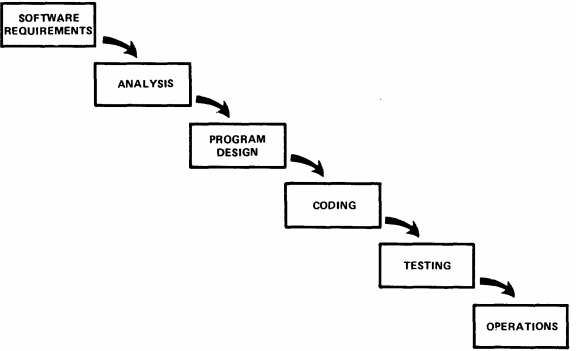
\includegraphics[scale=0.4]{Figurer/diagram/waterfall-model.png}
    \caption{Vannfallsmodellen beskrevet av Winston Royce}
    \source{\cite{royceManagingDevelopmentLarge1970}}
    \label{fig:waterfall-model}
  \end{minipage}
  \hfill
  \begin{minipage}[b]{0.45\textwidth}
    \centering
    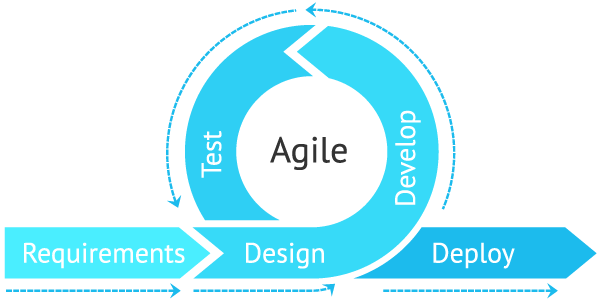
\includegraphics[scale=0.3]{Figurer/diagram/agile-dev.png}
    \caption{Modell over agil utvikling}
    \source{\cite{WhyAgileImportant2020}}
    \label{fig:agile-dev}
  \end{minipage}
\end{figure}
\noindent
Det ble bestemt i starten av utviklingsprosessen å gå for en agil utviklingsmetodikk framfor den mer tradisjonelle Vannfallsmetoden. Selv om utviklingsteamet bare består av to personer og applikasjonen har et nokså snevert og spesifisert omfang, var ikke kravspesifikasjonen fastsatt fra starten av. Mange av funksjonene og valg av teknologi ble tatt underveis i prosjektets løp ved å ha ukentlige møter sammen med professor Hvasshovd. Det var et behov å kunne tilpasse seg gjennom prosjektet. Ettersom utviklerne i tillegg hadde mer erfaring med agil metodikk, var slik metodikk bedre egnet for hele prosjektet, både for fordypningsprosjektet og masteroppgaven.

\subsection{Valg av agil metodikk}
Eksempler på noen av de mest kjente agile metodikkene er Scrum \cite{HomeScrumOrg}, Kanban og Extreme Programming \cite{wellsExtremeProgrammingGentle2009}. I dette prosjektet ble Scrum og Kanban vurdert. 
\newline
\newline
Scrum, som for alvor tok av etter boken \enquote{Agile software development with Scrum} \cite{schwaberAgileSoftwareDevelopment2002} i 2002, kjennetegnes ved at både kunder og utviklingsteam får roller med et bestemt ansvarsområde samt en rekke artefakter og hendelser som gjentas over prosjektets løp \cite{WhatScrum}. Prosjektet gjennomføres ved å deles inn i kortere iterasjoner kalt \textit{sprinter} \cite{WhatScrum} som er en fast leveransesyklus på 1-4 uker \cite{nesKortIntroduksjonTil2019}. Produkteierens ansvar er å lage en prioriert liste over produktets ønskede funksjonalitet, kalt \textit{backlog}, som det blir tatt utgangspunkt i når man skal lage en egen \textit{backlog} for \textit{sprinten} som skal gjennomføres \cite[~s.24]{rannikkoUserCenteredDesignAgile2011}. Utviklerteamet har ansvar for å implementere og potensielt levere et produkt eller funksjon for hver sprint og oppdatere \textit{backloggen} underveis ved hjelp av en Scrum-tavle som visualiserer oppgavene \cite[~s.24]{rannikkoUserCenteredDesignAgile2011}. Hver dag møtes utviklerne for korte \textit{standup}-møter der de forteller hva som har blitt gjort og hva som skal gjøres for dagen, slik at alle er oppdaterte \cite{WhatScrum}. Etter hver \textit{sprint} gjennomføres et refleksjonsmøte for å se hva som kan forbedres i prosessen til neste \textit{sprint} \cite{WhatScrum}. I tillegg får en av utviklerene en ekstra rolle som Scrum-master som skal sørge for at alle i teamet forstår og følger Scrum-praksis \cite[~s.24]{rannikkoUserCenteredDesignAgile2011}. 
\newline
\newline
Kanban oppstod på 1940-tallet da Toyota begynte å bruke det i deres fabrikker for å optimalisere arbeidsflyten. På 2000-tallet ble prinsippene utviklet hos Toyota overført til programvareutvikling \cite{radiganKanbanBriefIntroduction}. Det er en agil metodikk med et par likheter til Scrum. Det brukes blant annet også en tavle for å vise \textit{backlog}, pågående arbeidsoppgaver og utførte oppgaver eller andre egendefinerte lister \cite{radiganKanbanBriefIntroduction}. Kanban har et spesielt fokus på å optimalisere arbeidsflyt, maksimere effektivitet og unngå flaskehalser \cite{radiganKanbanBriefIntroduction}. Derfor benyttes det ikke tidsbestemte \textit{sprinter} slik som i Scrum, men en kontinuerlig flyt av arbeid og distribusjon \cite{radiganKanbanBriefIntroduction}. Det er heller ingen faste roller for de involverte i prosjektet. Pågående oppgaver for hver arbeidskategori blir begrenset slik at utviklerne ikke påtar seg for mange oppgaver samtidig og stagnerer fremdriften i prosjektet \cite{radiganKanbanBriefIntroduction}. Om antall pågående arbeidsoppgaver er på den fastsatte maksgrensen for påbegynte oppgaver, må en utvikler hjelpe til med de påbegynte oppgavene før en ny oppgave kan startes på \cite{radiganKanbanBriefIntroduction}. 
\newline
\newline
Selv om utviklerne hadde mest erfaring med å utvikle med Scrum både i skole- og arbeidssammenheng, ble det sett på som lite hensiktsmessig med tanke på at det bare var to utviklere i prosjektet. Det ville vært vanskelig å utfylle alle arbeidsrollene og ført til unødvendig bruk av tid med \textit{standup-} og refleksjonsmøter når utviklerne under så og si hele utviklingsprosessen var i samme rom og kunne holde hverandre oppdatert kontinuerlig. Å utvikle i \textit{sprinter} ble også valgt bort ettersom det hadde vært tidkrevende å planlegge disse sammen med produkteier professor Hvasshovd annen hver uke. Kanban ble derfor et naturlig valg for dette prosjektet med mulighet for kontinuerlig flyt, fravær av bestemte arbeidsroller og visualisering samt begrensning av arbeidsoppgaver som gjorde det enklere å få øye på flaskehalser i utviklingsprosessen. 

\subsubsection{Trello}
En essensiell del av Kanban er tavlen som visualiserer arbeidsoppgavene. Dette kan være en fysisk liste med klistrelapper eller digitale tavler. Under dette prosjektet ble samhandlingsverktøyet Trello \cite{Trello} benyttet ettersom det kunne bli brukt i sanntid av begge utviklerne og la til rette for bruk av fargekoder slik at oppgavene kunne kategoriseres både for utvikling av programkode, skriving av oppgaven og andre egendefinerte kategorier. Det faktum at tavlen kunne oppdateres i sanntid gjorde også enklere for utviklerne å være oppdatert på hva den andre personen arbeidet med i de periodene utviklerne hadde hjemmekontor hver for seg. Utviklerne valgte å sette maksgrensen for påbegynte arbeidsoppgaver til tre, som det er mulig å se i figuren under i listen WIP (Work in Progress). 
\begin{figure}[H]
\centering
\captionsetup{width=.8\linewidth}
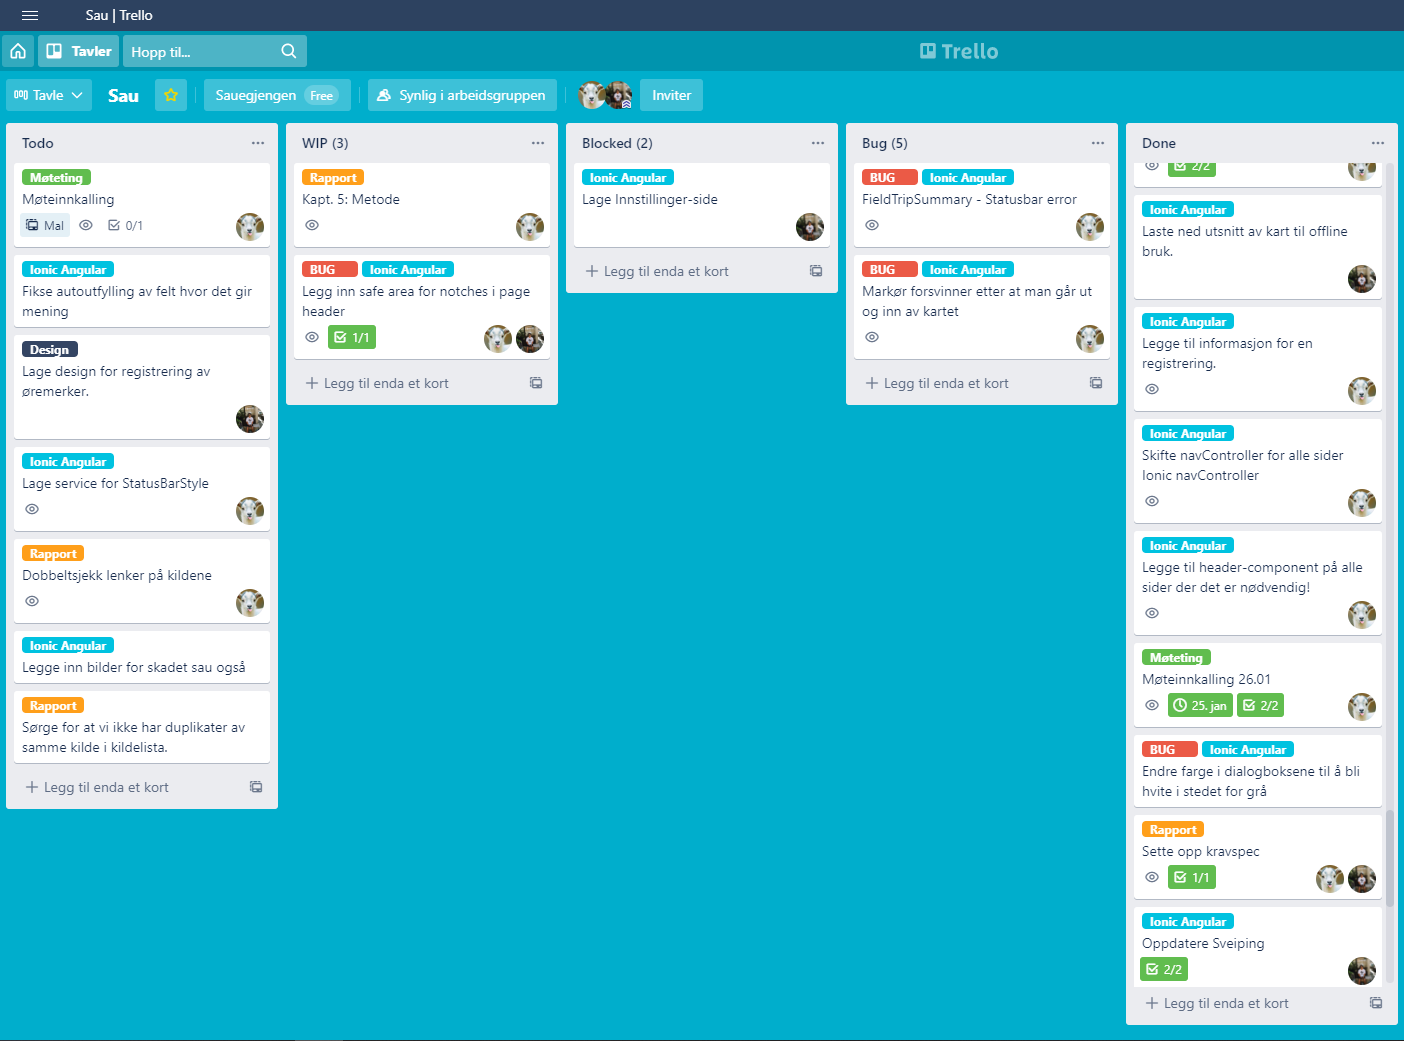
\includegraphics[scale=0.4]{Figurer/Bilder/trello.png}
\caption{Skjermbilde av Trello-tavlen under prosjektet.}
\label{fig:trello}
\end{figure}

\section{Konklusjon}
% Forskningsmetoden brukt i dette prosjektet for å innhente informasjon og kunnskap om oppsyn av sau ble gjennomført med ukentlige møter med veileder og litteratursøk på internett.
Det ble bestemt å bruke en agil utviklingsmetodikk og ikke den mer tradisjonelle Vannfallsmodellen. Dette er grunnet at kravspesifikasjonene ikke var satt før prosjektets start men utviklet underveis, og agil metodikk er svært tilpasningsdyktig i motsetning til Vannfallsmodellen som er mer rigid. Av mange ulike agile metodikker falt valget på Kanban som passet best det et lite utviklingsteam med dets kontinuerlige flyt av arbeid, fravær av bestemte roller for de involverte i prosjektet samt visualisering og begrensning av arbeidet som vises på en tavle.  Samhandlingsverktøyet Trello ble benyttet som en digital Kanban-tavle.
\chapter{Valg av metode}
Dette kapitlet beskriver valget av metode for med tanke på forskningsdelen av prosjektet. En forskningsplan har blitt utformet i henhold til rammeverket utviklet av Oates \cite{oatesResearchingInformationSystems2013} i boken \textit{Researching Information Systems and Computing}. Her beskriver hun utviklingen av en forskningsplan og deler det inn i seks deler kalt \textit{The 6Ps of Research} (De 6 P-ene innenfor forsknings): \textit{Puropse} (Formål), \textit{Products} (Produkter), \textit{Process} (Prosess), \textit{Participants} (Deltakere), \textit{Paradigm} (Paradigme) og \textit{Presentation} (Presentasjon). Paradigme vil ikke bli diskutert da det ikke er nødvendig ettersom at dette i hovedsak er et systemutviklingsprosjekt.

\section{Formål}
Her beskrives bakgrunnen for prosjektet, samt tidligere forskning innenfor samme felt. Det forklares hva som skiller vår forskning fra eksisterende forskning, og til slutt vil forskningsspørsmålene for prosjektet bli presentert.
\newline
\newline
\noindent
Bakgrunnen for oppgaven blir beskrevet i kapittel \ref{bakgrunn} \nameref{bakgrunn} og formålet blir beskrevet i underkapittel \ref{sec:mal-for-oppgaven} \nameref{sec:mal-for-oppgaven}. For å oppsummere er målet med oppgaven å utvikle en applikasjon som kan ta over for dagens løsning med penn og papir i forbindelse med registrering av informasjon under en oppsynstur. Applikasjonen som skal utvikles må både dekke dagens behov, men også tilby en løsning for blind interaksjon med en hånd mens brukeren ser gjennom en kikkert og gjøre det mulig for gjetere og bønder å dele informasjon innad i et beitelag. Tidligere forskning og løsninger innfor samme område inkluderer applikasjonen Beitesnap \cite{BeitesnapRevolusjonerendeVerktoy} av Fant AS fra 2017, et verktøy laget for å registrere observasjoner av husdyr på beitet. Et annet eksempel på tidligere arbeid er masteroppgaven \textit{Effektivisering av manuell oppfølging av sau på utmarksbeite} hvor Dysthe og Kjerstad \cite{dystheEffektiviseringAvManuell2018} utforsker en løsning for registrering av saueflokker i forbindelse med oppsynsturer. Det som skiller denne løsningen fra tidligere arbeid er at den vil gi brukerne muligheten til å registrere saueflokker blindt med en hånd mens brukeren ser gjennom en kikkert. Dette er nødvendig da sauflokkene på utmarksbeitet ofte er så langt unna at man ikke klarer å registrere nødvendig informasjon uten å ta i bruk kikkert. Løsningen vil også være kryssplattform og fungere på mobile enheter som kjører både iOS og Android, noe som ble forsøkt av Dysthe og Kjerstad \cite{dystheEffektiviseringAvManuell2018} i 2018, men ble ikke fullført.
\newline
\newline
\noindent
I løpet av prosjektet vil det utvikles en fullverdig, fungerende versjon av en applikasjon som kan kjøre på både iOS og Android. Applikasjonen skal deretter brukertestes for å finne potensielle svakheter i designet. Ved å gjøre dette er det et ønske å svare på følgende forskningsspørsmål:

\begin{itemize}
    \item \textbf{F1: Hvordan utvikle et digitalt verktøy for å bistå sauebønder, beitelag og gjetere på oppsynstur slik at arbeidet med manuell registrering blir mer effektivt og raskere?}
    \item \textbf{F1.1: Kan man lage et system som erstatter dagens løsning med penn og papir, men fortsatt dekker alle brukerens behov?}
    \item \textbf{F1.2: Hvordan kan et digitalt system bistå sauebonde, beitelag og gjetere slik at de kan samhandle og dele informasjon om oppsynsturer med hverandre og norske myndigheter?}
    \item \textbf{F1.3: Hvordan utvikle et brukergrensesnitt som muliggjør registrering av sau uten å måtte se på mobilskjermen?}
    \item \textbf{F1.4: Hvordan utvikle et brukergrensesnitt som muliggjør registrering av sau under alle værforhold?}
\end{itemize}

\section{Produkter}
Dette underkapitlet forklarer hvilke produkter som vil komme som et resultatet forskningsprosjektet.
\newline
\newline
\noindent
Hovedproduktet fra forskningen vil være en applikasjon som kan erstatte dagens løsning for registrering av informasjon om saueflokker på utmarksbeitet med penn og papir. Samtidig skal applikasjonen tilby utvidet funksjonalitet med tanke på informasjonsflyt og brukbarhet. Selv om hovedmålet med prosjektet er å utvikle en applikasjon, vil resultatene både fra fordypningsprosjktet og selve masteroppgaven være med på å bidra til økt kunnskap om både utvikling av brukergrensesnitt for blind bruk, samt utvikling av kryssplattform-applikasjoner for bruk i forbindelse med informasjonsregistrering hvor man ikke har tilgang til internett der GPS og kart spiller en hovedrolle.

\section{Prosess}
Underkapittelet om prosess beskriver planen for hvordan det er tenkt å gå fram med forskningen under prosjektet. Prosessen baserer seg på figur \ref{fig:research_process} hentet fra \textit{Researching Information Systems and Computing} \cite{oatesResearchingInformationSystems2013}.
\newline
\newline
\noindent
Arbeidet med prosjektet var motivert av ønsket om å lage en applikasjon, utviklet basert på eksisterende litteratur, løsninger og forskning som kunne være med og bidra til å redusere antall sauer som dør hvert år på utmarksbeitet, samt gjøre arbeidshverdagen til sauebonder og gjetere enklere. Prosjektet startet med et litteratursøk inn i eksisterende løsninger for denne typen applikasjoner. Det ble også gjort et grundig arbeid for å kartlegge brukerens behov, basert både på dagens løsning men også hva som kreves fra myndighetens side. Dette både for å hjelpe til med å forme forskningsspørsmål, mens også for å kunne danne et konseptuelt rammeverk for prosjektet. 
\begin{figure}[H]
\centering
\captionsetup{width=.8\linewidth}
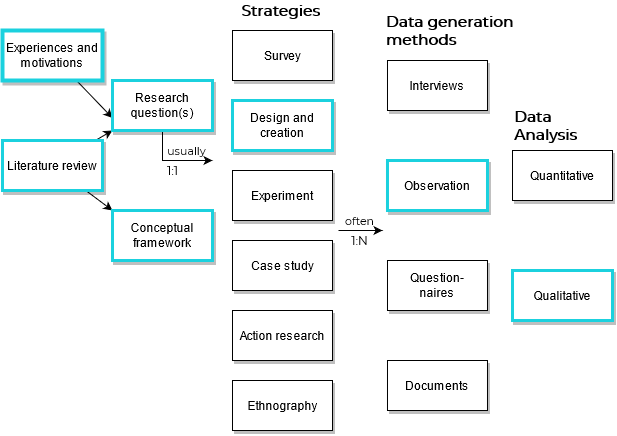
\includegraphics[scale=0.6]{Figurer/diagram/research_process.png}
\caption{Figuren viser den valgte veien for forskningsprosess markert med fargede bokser.}
\label{fig:research_process}
\source{\cite[~s.33]{oatesResearchingInformationSystems2013}}
\end{figure}

\noindent
Planen er å bruke \textit{Design og creation}-strategien for å implementere en applikasjon basert både på resultatene fra fordypningsprosjektet og litteratursøket. Når en ferdig førsteversjon av applikasjonen har blitt utviklet planlegger vi å brukerteste denne på fem ulike brukere. Her vil vi bruke \textit{Observation} som metode for å generere data fra brukertestene. Etter at testene er utført vil det bli gjort en kvalitativ analyse av dataene.

\section{Deltagere}
Dette kapitlet beskriver deltakerne i prosjektet og deres roller.
\newline
\newline
\noindent
Hoveddeltakerne i dette prosjektet vil være de som utfører selve prosjektet, altså Kimia Dadar Abtahi og Trym Vegard Gjelseth-Borgen. Personen som kommer til å veilede oss gjennom prosjektet, gi nyttig erfaringsbasert informasjon med tanke på oppsynsturer og som vil fungere som produkteier er Professor Svein-Olaf Hvasshovd. Det vil også være fem testdeltakere som deltar for å hjelpe til med brukertestene av applikasjonen. Data fra brukertestene og om testdeltakerne vil være anonymisert.

\section{Presentasjon}
Underkapitlet om presentasjon beskriver hvordan resultatene fra forskningsprosjektet vil bli presentert etter endt prosjekt.
\newline
\newline
\noindent
Resultatet av forskningen vil bli presentert i masteroppgaven. Resultatene vil også kunne være med på å utvikle en forbedret versjon av applikasjonen, hvis dette skulle være ønskelig etter prosjektets slutt.
\chapter{Valg av teknologi}
Dette kapitlet gjennomgår teknologien som ble valgt til å utvikle applikasjonen, teknologien som ble vurdert men ikke valgt og årsaken til valgene som ble gjort. For at applikasjonen skulle ha mulighet til å nå kravene spesifisert i kravspesifikasjonen var det viktig å vurdere nøye hvilke teknologier som passet best til den gitte problemstillingen.

\section{Utviklingsrammeverk}
Under valget av utviklingsrammeverk var det to faktorer som var spesielt viktig å ta med inn i vurderingen. De spesifikke kravene det siktes til er det funksjonelle kravet F1 beskrevet i tabell \ref{tbl:funksjonelle-krav} og det ikke-funksjonelle kravet IF2 beskrevet i tabell \ref{tbl:ikke-funksjonelle-krav}. F1 og IF2 handler henholdsvis om at utviklingsrammeverket må gjøre det mulig å implementere et kartgrensesnitt ved hjelp Kartverkets tjenester og at det skal være mulig å lage en kryssplattform applikasjon som skal fungere på både iOS og Android.

\subsection{Krav om en kryssplattform-applikasjon}
På bakgrunn av det ikke-funksjonelle kravet IF2 var det flere ulike utviklingsrammeverk som ble vurdert. Likt for alle rammeverkene som ble vurdert var det at de tilbyr utvikling av en applikasjon for både iOS og Android med bare én kodebase. Ved å bare ha én kodebase vil utviklingstiden kunne reduseres betraktelig ettersom at man slipper å lage den samme applikasjonen to ganger. Framtidig vedlikehold og oppdateringer vil også være lettere og raskere å utføre. Utviklingsrammeverkene som ble vurdert til applikasjonen var Flutter \cite{FlutterBeautifulNative} utviklet av Google, NativeScript \cite{NativeScript} som er et utviklingsrammeverk for kryssplattformutvikling med åpen kildekode, React Native \cite{ReactNativeFramework} laget av Facebook basert på JavaScript-rammerverket React \cite{ReactJavaScriptLibrary} og Ionic \cite{IonicCrossPlatformMobile} som er et kryssplattformrammeverk spesielt laget for mobile enheter. Alle disse ulike utviklingsrammeverkene tilbyr funksjonalitet for å lage en applikasjon for både iOS og Android med bare én kodebase. Likevel vil det alltid oppstå situasjoner hvor man er nødt til å skrive plattformspesifikk kode og disse situasjonene oppstår oftere hos noen rammeverk enn hos andre. Av de nevnte rammeverkene er Ionic det rammeverket som krever minst plattformspesifikk kode, mens React Native krever mest plattformspesifikk kode. Flutter og NativeScript havner en plass midt i mellom disse to \cite{FrameWorkComparison}. Ionic er også et av rammeverkene med flest ferdiglagde brukergrensesnitt-komponenter, noe som gjør at man under utvikling kan bruke mindre tid på grensesnittspesifikk implementasjon og mer tid på implementasjon av funksjonalitet. React Native har minst ferdiglagde komponenter mens Flutter stiller likt med Ionic. NativeScript havner en plass mellom Ionic og React Native \cite{FrameWorkComparison}.

\subsection{Krav om integrasjon med NorgesKart}
Det funksjonelle kravet F1 beskrevet i tabell \ref{tbl:funksjonelle-krav} beskriver at løsningen krever at kartet i applikasjonen bruker Kartverkets løsninger i form av tjenesten NorgesKart. Geonorge, som er det det nasjonale nettstedet for kartdata og annen stedfestet informasjon i Norge \cite{OmGeonorge}, linker til JavaScript-biblioteket Leaflet \cite{LeafletJavaScriptLibrary} i deres brukerveiledning om bruk av Kartverkets tjenester \cite{GeoNorgeLeaflet}. Også tidligere forsøk på implementasjon av en lignende applikasjon har brukt JavaScript-biblioteket Leaflet for å vise fram kartdata \cite[~s.116]{dystheEffektiviseringAvManuell2018}. For at implementasjonen av kartgrensesnittet i applikasjonen skulle gå så smertefritt som mulig ble det ble derfor tidlig bestemt at Leaflet skulle brukes. Derfor ble det viktig at utviklingsrammeverket støttet bruk av Leaflet. Flutter skrives i språket Dart \cite{FlutterDart} og støtter derfor ikke bruk av JavaScript-bibliotek Leaflet ettersom at Dart og JavaScript ikke er kompatible. Leaflet trenger direkte tilgang til et DOM-element \cite{IntroductionDOMWeb} for å legge selve kartet inn i brukergrensesnittet \cite{LeafletDom}. Selv om React Native skrives i språket JavaScript, støtter ikke React Native JavaScript-biblioteker som trenger direkte tilgang til DOM-elementer \cite{JavaScriptLibraryReactNative}. Det ble derfor ikke aktuelt å bruke hverken Flutter eller React Native i løsningen. Både Ionic og Native Script støtter bruk av JavaScript-rammerverket Angular \cite{IonicAngularOverview, NativeScriptAngular} for å lage brukergrensesnitt i applikasjonen. Angular støtter direkte tilgang til DOM-elementer \cite{AngularElementRef} i tillegg til at det støtter bruk av JavaScipt-bibliotek \cite{AngularJavaScriptLibraries}, noe som gjør at Leaflet vil fungere i både Ionic og NativeScript.

\subsection{Ionic + Capacitor}
Valget for hvilket utviklingsrammeverk som skulle brukes i applikasjonen falt til slutt på Ionic. Selv om NativeScript var en mulig kandidat, ble det bestemt å bruke Ionic ettersom at det potensielt kunne resultere i en mindre og lettere vedlikeholt kodebase og fordi Ionic har flere ferdiglagde brukergrensesnittkomponenter å velge mellom enn NativeScript \cite{FrameWorkComparison}. Ionic er en hybrid utviklingsplattform med åpen kildekode som kom på markedet i 2013 \cite{IntroducingIonicIonic}. Den gjør det mulig å lage kryssplattform-applikasjoner med web-teknologi og støtter de mest kjente JavaScript-rammerverkene som Angular, Vue.js og React, samt vanlig HTML, CSS og JavaScript \cite{IonicCrossPlatformMobile}. For at kode utviklet med web-teknologi skal kjøre på mobile eneheter og ha tilgang til maskinvare-funksjonalitet som mobilenes kamera eller GPS trengs det et mellomledd som binder sammen web-applikasjonen og maskinvaren \cite{CapacitorBlogHow}. Capacitor \cite{CapacitorCrossplatformNative} og Cordova \cite{ApacheCordova} er eksempler på slike mellomledd. Det ble besluttet å bruke Capacitor i utviklingen av denne applikasjonen. Årsaken til dette er at Capacitor er mer brukt, har 99\% bakoverkompatibilitet med utvidelser fra Cordova og fordi Capacitor kom ut i 2018 og bruker nyere moderne API-er som ikke var tilgjengelig da Cordova kom ut i 2009 \cite{CordovaVsCapacitor}. 

\begin{figure}[H]
\centering
\captionsetup{width=.8\linewidth}
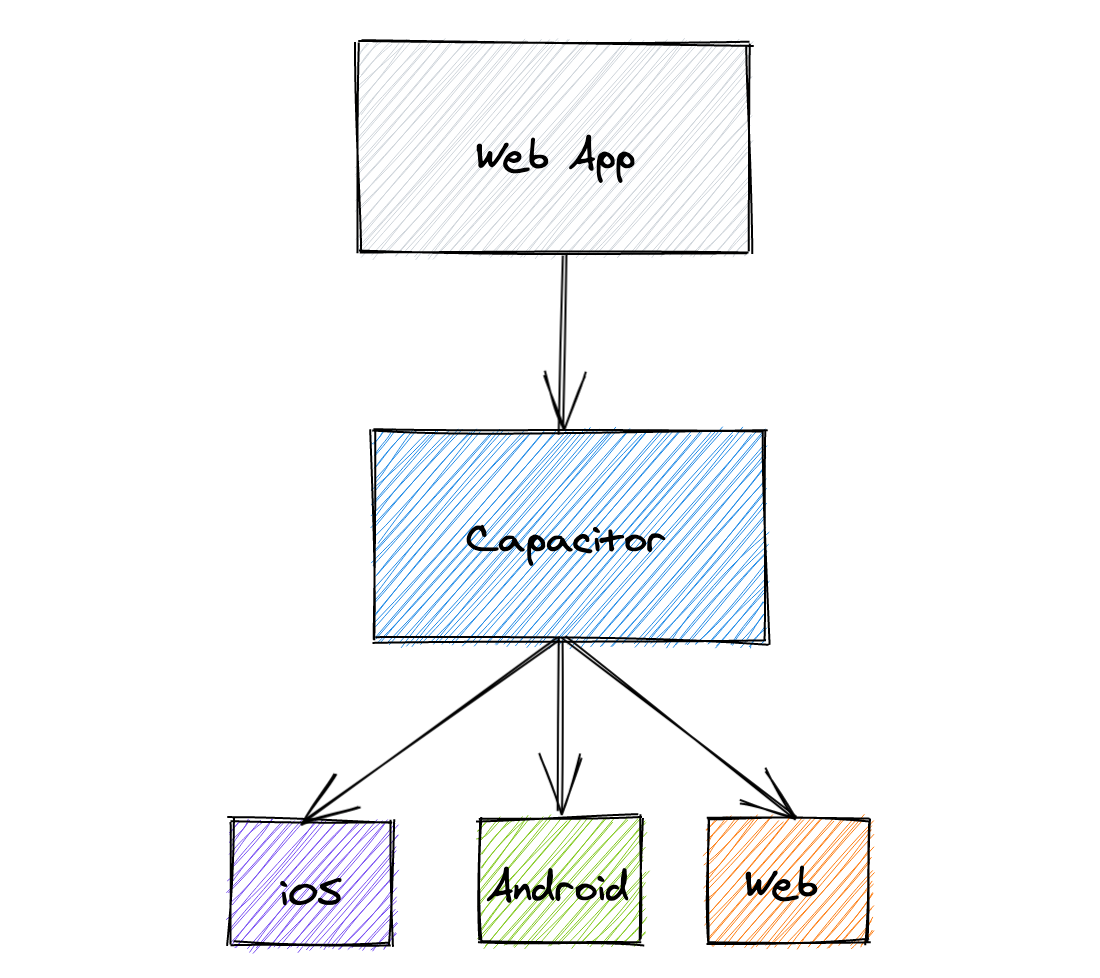
\includegraphics[scale=0.5]{Figurer/Bilder/capacitor-figure.png}
\caption{Forenklet figur som viser oppbygningen av en applikasjon som bruker web-teknologi sammen med Capacitor.}
\label{fig:how-capacitor-works}
\source{\cite{CapacitorBlogHow}}
\end{figure}

\section{Biblioteker}
\subsection{Frontend-bibliotek}
Ionic støtter bruk av flere forskjellige JavaScript-rammerverk for utvikling av web-applikasjon-delen av mobilapplikasjonen, samt støtte for vanlig HTML, CSS og standard JavaScript \cite{IonicCrossPlatformMobile}. JavaScript-rammeverkene som støttes per dags dato (17.03.2021) er Angular utviklet av Google \cite{Angular}, React utviklet av Facebook \cite{ReactNativeFramework} og Vue.js som er et uavhengig JavaScript-rammeverk med åpen kildekode \cite{VuejsVue2021}. Under utviklingen av litt større web-applikasjoner lønner det seg å bruke et JavaScript-rammeverk framfor å bruke standard HTML, CSS og JavaScript. Etterhvert som applikasjoner vokser kreves det flere filer og mer kode per fil. Å holde kontroll på disse på egenhånd ved hjelp av mapper og ryddig kode blir etterhvert vanskelig og kan føre til et spaghettilignende rot. De nevnte JavaScript-rammeverkene er laget for å holde koden i sjakk, gjøre det mulig å lage gjenbrukbare komponenter som fører til redusert kode og gir applikasjonen rom til å vokse mens den samtidig er lett å vedlikeholde \cite{aboutJavaScriptFrameworks}. En av ulempene med slike JavaScript-rammeverk er at de kan ha en relativt bratt læringskurve. Ettersom at begge prosjektdeltagerne hadde erfaring med utvikling med JavaScript-rammeverk fra før av ble denne problemstillingen ikke tatt i betraktning.
\newline

\noindent
Når det kom til valget av hvilket spesifikke rammeverk som skulle brukes stod det mellom React og Angular. Når applikasjonen ble påbegynt høsten 2020 var Ionic med Vue.js enda i Beta-versjon \cite{AnnouncingNewIonic} og ble derfor ikke sett på som et alternativ. Vi endte til slutt med å bruke Angular da Angular tilbyr strengere form for kodestruktur hvor HTML, CSS og JavaScript/TypeScript er delt opp i hver sin fil. Angular tilbyr også mulighet for å bruke TypeScript \cite{TypeScriptTypedJavaScript}, en versjon av JavaScript som gjør det mulig å typesette koden for økt struktur og enklere debugging \cite{AngularWhatAngular}.

\subsection{NGXS} \label{sub:ngxs}
Under planleggingen av applikasjonen ble det sett på som nødvendig å implementere en form for tilstandshåndtering for brukergrensesnittet. Applikasjonens flyt, spesielt under registrering av en saueflokk (se underkapittel \ref{subsubsec:registrering av sau} \nameref{subsubsec:registrering av sau}), består av flere ledd hvor å holde kontroll på antall registrerte søyer og lam med forskjellig farge, slips og øremerker er kritisk for at registreringen skal bli korrekt og brukeropplevelsen skal blir så bra som mulig. For å få til dette ble det valgt å bruke tilstandsbiblioteket NGXS \cite{IntroductionNGXS}. NGXS er modulert etter det populære tilstandsbiblioteket Redux laget for React, men reduserer redundant \textit{boilerplate}-kode ved å ta i bruk moderne TypeScript-funksjonalitet som klasser og dekoratører \cite{IntroductionNGXS}. Dataflyten ved bruk av NGXS illustreres i figur \ref{fig:ngxs-illustration}. Her referer \textit{Components} til ulike komponenter i brukergrensesnittet. \textit{Store} er den lagrede  tilstanden til applikasjonen, mens \textit{Actions} er handlinger utført av \textit{Components} som \textit{muterer} tilstanden i \textit{Store}. Når en komponent utfører en \textit{Action} og muterer en verdi i \textit{Store}, vil alle komponenter som tar i bruk den muterte verdien få beskjed om dette slik at komponentene får mulighet til å hente den siste tilgjengelige tilstanden. Applikasjonen består av flere ulike komponenter som har ansvaret for forskjellige funksjonalitet som for eksempel å lese opp tekst til brukeren under blind registrering (text-to-speech), ta i mot input fra brukeren eller vise hva som er registert i en oppsummering på skjermen. For at alle disse ulike komponentene skulle ha tilgang den samme informasjonen ble bruken av NGXS essensiell.
\begin{figure}[H]
\centering
\captionsetup{width=.8\linewidth}
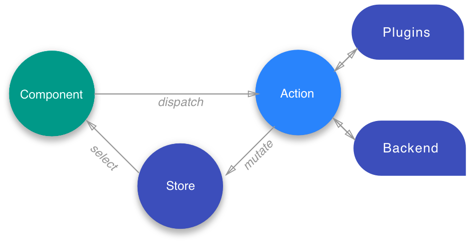
\includegraphics[scale=0.5]{Figurer/Bilder/ngxs-figure.png}
\caption{Dataflyt ved bruk av NGXS.}
\label{fig:ngxs-illustration}
\source{\cite{ngxsIllustration}}
\end{figure}

\subsection{Tekstopplesning}
For at applikasjonen skulle nå det funksjonelle kravet F4.1 \textit{Brukeren skal få verbale tilbakemeldinger om utførte handlinger underblind bruk slik at brukeren slipper å se på skjermen} beskrevet i tabell \ref{tbl:funksjonelle-krav} var det nødvendig å implementere en form for stemme som kunne gjengi informasjon vist på skjermen. Her sto valget mellom å enten bruke en tekstoppleser ofte brukt for blinde eller svaksynte, eller å spille inn en rekke lyder som kunne mikses og spilles av for å lese opp informasjon fra applikasjonen. Her falt valget på å bruke en tekstoppleser ettersom å spille inn lyder for hver eneste situasjon kom til å ta utrolig lang tid, samt at lydfilene ville brukt en del lagringsplass. Selv om dette kanskje ikke var tilfellet før har nå både iOS og Android innebygd støtte for tekstopplesning, ettersom at det gir økt tilgjengelighet for svaksynte og blinde \cite{TextToSpeechAndroidDevelopers, AVSpeechSynthesizerAppleDeveloper}. Det ville også gjort applikasjonen dårlig utrustet for eventuelle endringer eller utvidelser ettersom det da måtte brukes tid på spille inn nye lydfiler.
\newline

\noindent
Etter et forsøk på å implementere den sammfunnsutviklede Capacitor-utvidelsen \textit{capacitor-community/text-to-speech} \cite{CapacitorcommunityTexttospeech2021} i applikasjonen, kom det fram at den ikke hadde den funksjonaliteten som var ønsket for opplesing av tekst på iOS. For at brukeropplevelsen skulle bli så bra som mulig var det et behov for å kunne avbryte en tekst-opplesning før den var ferdig, og starte på opplesning av ny tekst. Dette fungerte utmerket på Android, men lot seg ikke gjøre i iOS med denne utvidelsen. Det ble derfor tatt en beslutning på å lage en egen utvidelse til Capacitor for tekstopplesning, ettersom at dette er sentral funksjonalitet i applikasjonen. Gjennom Capacitor er det heldigvis enkelt å utvikle og teste egne utvidelser både på Android og iOS \cite{CreatingCapacitorPlugins}. Utvidelsen \textit{capacitor-tts-plugin} ble laget for bruk i applikasjonen og er publisert på npmjs.com (\url{https://www.npmjs.com/package/capacitor-tts-plugin}), noe som gjør at man enkelt kan installere og bruke utvidelsen i sitt eget prosjekt ved hjelp av NPM \cite{NpmNpmDocs}. 


\section{Backend-løsning}
For at samhandling mellom brukere av applikasjonen skulle være mulig ble det behov for en form autentisering av brukere og sentral lagring av registrerte oppsynsturer. Det finnes mange ulike måter å gjøre dette på. Løsningene som ble vurdert for denne applikasjonen var enten Googles skybaserte løsning Firebase \cite{Firebase} eller en kombinasjon av rammeverket Node.js \cite{NodeJs} for å lage en tjener med MongoDB \cite{MongoDBAtlasCloud} som databaseløsning. Valget falt til slutt på Firebase da det er svært enkelt å bruke, ikke har behov for en tjener og tar seg av autentisering og lagring eksternt i skyen. Kombinasjonen av en dedikert tjener med en ekstern dokument-database som MongoDB kunne passet utmerket til prosjektet da det gir flere muligheter og større frihet. Likevel krever en slik løsning både mer midler i form av ekstra maskinvare for å rulle ut tjenerkoden på, samt ekstra tid for implementering. Det ble derfor sett på som mer hensiktsmessig å gå for Firebase.

\subsection{Firebase}
Firebase ble laget av Firebase Inc i 2011 \cite{FirebaseCrunchbaseCompany}, før det ble kjøpt opp av Google i 2014 \cite{GoogleAcquiresFirebase}. Firebase er en BaaS, Backend-as-a-Service, som gjør at man istedenfor å lage sin egen tjener-løsning/backend, har mulighet til å bruke tjenesten Firebase for alle tjener-relaterte oppgaver \cite{WhatBaaSBackendasaService}. Dette gjelder alt fra autentisering med Firebase Authentication, lagring med Cloud Firestore eller maskinlæring med Firebase Machine Learning \cite{FirebaseProducts}.

\subsubsection{Cloud Firestore}
For lagring av brukere, beitelag og registrerte oppsynsturer bruker applikasjonen Cloud Firestore. Cloud Firestore er en NoSQL-database som lagrer filer/dokumenter på JSON-format i skyen. Cloud Firestore lagrer data i en 3-delt struktur. \textit{Data}, i form av JSON, lagres i \textit{documents}, som igjen lagres \textit{collections}. En \textit{collection} kan ha en eller flere dokumenter, men et \textit{document} har også mulighet til å peke til nye \textit{collections} \cite{CloudFirestoreFirebase}. Systemet gjør det altså mulig å lagdele data som lagres i databasen for struktur og logikk. Dette var funksjonalitet som var nødvendig i vårt tilfelle ettersom vi ønsket å dele inn tilgang på registrerte oppsynstur basert på brukere og beitelag.
\begin{figure}[H]
\centering
\captionsetup{width=.8\linewidth}

\includegraphics[scale=0.4]{Figurer/Bilder/structure-data-firestore.png}
\caption{Datastruktur i Cloud Firestore.}
\label{fig:firestore-datastrktur}
\source{\cite{CloudFirestoreFirebase}}
\end{figure}

\subsubsection{Firebase Authentication}
Firebase Authentication er Firebase sin løsning for autentisering i skyen. Tjenesten støtter innlogging gjennom Facebook, Google, Twitter osv, men også innlogging med brukernavn og passord. Data for den innloggede brukeren lagres i skyen og brukes til autentisering når en bruker prøver å lese eller skrive til en fil i Cloud Firestore. Den eneste funksjonaliteten som trenger å bli implementert på selve enheten er en innloggings-side som sender brukernavn og passord til Firebase Authentication \cite{FirebaseAuthenticationSimple}. Ved å velge Firebase Authentication for autentisering ble en prosess som erfaringsmessig tar lang tid, gjort på bare én dag. Dette gjorde at vi kunne bruke mer tid på implementasjon av viktig funksjonalitet i andre deler av applikasjonen.

\section{Konklusjon}
For utvikling av selve grensesnittet ble utviklingsrammeverket Ionic sammen med JavaScript-rammeverket Angular valgt. Det ble her funnet ut at Ionic passet best for utvikling av denne applikasjonen basert på kravene presisert i kravspesifikasjonen. For å få tilgang til \textit{native}-funksjonalitet på mobiltelefonene applikasjonen skal kjøre på brukes Capacitor, da det var det mest moderne alternativet med mest funksjonalitet. Tilstandshåndteringen i applikasjonen tas hånd om av biblioteket NGXS, da det er laget for Angular og krever mindre \textit{boilerplate}-kode en tilsvarende bibliotek. For at applikasjonen skulle håndtere tekst-opplesning likt på både iOS og Android ble det utviklet en egen utvidelse til Capacitor for tekstopplesning som nå ligger ute i NPM-registeret for enkel bruk. Backend-løsningen i applikasjonen er gjort med en Backend-as-a-Service i form av Firebase, da det tilbyr all ønsket funksjonalitet mens det samtidig ga kortest mulig implementasjonstid.
\chapter{Design} \label{cha:Design}
Dette kapitlet tar for seg prosessen rundt designet av brukergrensesnittet til applikasjonen, resultatene som følge av designfasen og verktøyene som ble tatt i bruk under prosessen og utviklingen av grensesnittene.

\section{Verktøy}
\subsection{Coolors}
For å gjøre fargevalg for applikasjonens elementer enklere ble verktøyet Coolors fra coolors.co brukt \cite{BianchiCoolorsGenerator}. Verktøyet gjør det mulig å generere ulike fargepaletter helt fra bunnen av, men også med utgangspunkt i enkeltfarger. Verktøyet har også funksjonalitet for å hente ut fargene man finner på flere forskjellige formater, som blant annet hex \cite{ColorsHEX} og rgb \cite{ColorsRGB} som er veldig vanlige formater for å beskrive farger i utviklingsverdenen.

\subsection{Affinity Designer}
Under utvikling av applikasjonen viste det seg at det ble et behov for ikoner og illustrasjoner for bruk i applikasjonen som ikke lot seg lage i HTML eller CSS. For å unngå unødvendige kostnader ble valgt å utvikle disse elementene fra bunnen av framfor å bruke gratis dårlige ferdiglagde utgaver eller å betale for bra utgaver. For design av disse elementene ble verktøyet Affinity Designer \cite{AffinitySoftware} brukt. Affinity Deisgner er et designverktøy som brukes for å lage ulike grafikker, logoer, ikoner med mer og kan sammenlignes med det mer kjente Illustrator fra Adobe \cite{BransjeledendeIllustrator}. Affinity Designer ble i hovedsagt valgt fordi prosjektdeltakerne allerede hadde erfaring og tilgang til programvaren.

\subsection{Figma}
For å gjøre den programmatiske utviklingen av brukergrensesnittet mer effektivt ble det gjort et valg på at alle de ulike sidene av grensesnittet i applikasjonen først skulle tegnes i et design- og prototypeverktøy. Valget falt her på verktøyet Figma \cite{Figma:Tool.}. Andre verktøy som Adobe XD \cite{AdobeTool} og Balsamiq \cite{BalsamiqBalsamiq} ble også vurdert. Her ble det fordelaktig å velge Figma foran både Adobe XD og Balsamiq. Adobe XD og Figma er ganske like i funksjonalitet, men på grunn av tidligere erfaring i Figma ble Adobe XD valgt bort. Begge prosjektdeltakerne hadde erfaring med bruk av både Balsamiq og Figma. Det ble valgt å ikke bruke Balsamiq ettersom at det ikke tilbyr den ønskede funksjonaliteten da det er et mye enklere og mer primitivt verktøy.
\newline

\noindent
Figma gjør det mulig å designe fullstendige brukergrensesnitt som kan gjøres om til enkle prototyper for testing av basisfunksjonalitet. Figma er også laget for at det skal være enkelt å samarbeide og tilbyr funksjonalitet for å designe elementer sammen i sanntid over nettet.

\section{Resultater}
\subsection{Fargevalg}
Valget av fargepaletten i applikasjonen falt på en applikasjon med mørkt tema. Både fordi at det er populært i dagens applikasjonsmarked, men også fordi det kan føre til at applikasjonen på mobiler med OLED-skjermer \cite{OLEDOLED-Info} vil bruke mindre strøm under operasjon \cite{WhatEnerlytics}. Dette er viktig ettersom at applikasjonen skal kunne brukes lenge uten tilgang på strøm mens man går oppsynstur. Bakgrunnsfargen (hovedfargen) i applikasjonen er en mørk marineblå farge. Denne blir komplementert med en dus grønnfarge som blir brukt på knapper og enkelte andre elementer. Fargen på tekst gjennom nærmest hele applikasjonen er hvit. Fargevalget har resultert i en applikasjon hvor det er god kontrast mellom ulike elementer. Det er også god kontrast mellom de ulike elementene og tilhørende tekst. For å sørge for at applikasjonen er tilgjengelighet for personer med de vanligste formene for fargeblindhet brukte vi nettleserutvidelsen-utvidelsen Colorblinding \cite{LeonardoCardoso/Colorblinding:See.} under testing av ulike fargekombinasjoner.

\begin{figure}[H]
\centering
\captionsetup{width=.8\linewidth}
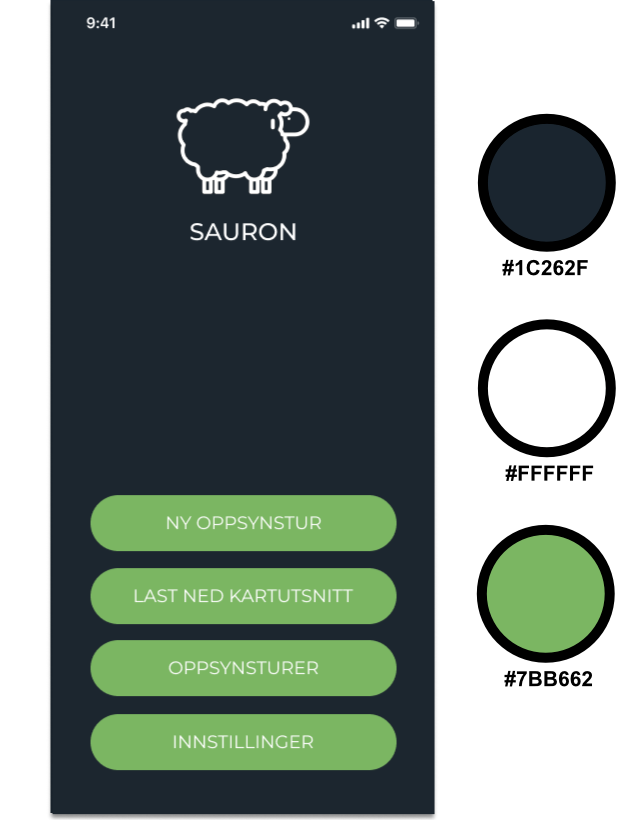
\includegraphics[scale=0.4]{Figurer/Bilder/valg-av-farger.png}
\caption{Illustrasjon av hovedmenyen i applikasjonen samt de ulike fargene brukt og deres tilhørende hex-verdier.}
\label{fig:valg-av-farger}
\end{figure}

\subsection{Nedlasting av kartutsnitt}
For å laste ned kartutsnitt kan man navigere seg til oversikten over nedlastede kartutsnitt fra hovedmenyen (figur \ref{fig:valg-av-farger}) ved å trykke på \enquote{Last ned kartutsnitt}-knappen. Oversikten viser alle nedlastede kartutsnitt, hvor mye plass kartutsnittene tar på mobilen og når de ble lastet ned.

\begin{figure}[H]
\centering
\captionsetup{width=.8\linewidth}
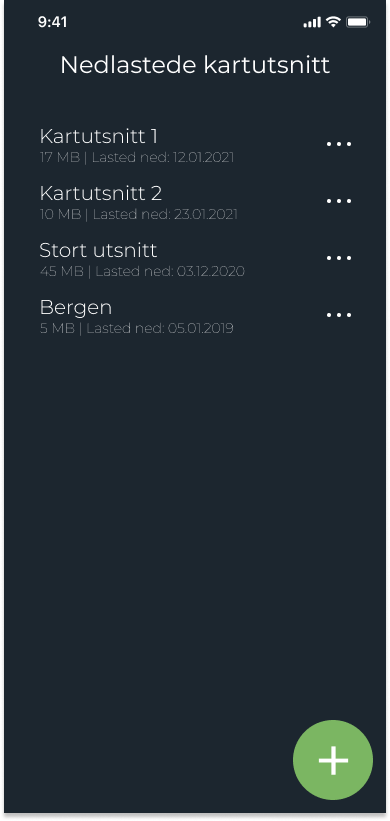
\includegraphics[scale=0.4]{Figurer/Figma/Frame 4 - Nedlastede kartutsnitt.png}
\caption{Prototypedesign av side for oversikt over nedlastede kartutsnitt.}
\label{fig:figma-nedlastede-kartutsnitt}
\end{figure}
\noindent
De tre prikkene på høyresiden av hvert nedlastede kartutsnitt kan trykkes på for å åpne en valgmeny (figur \ref{fig:figma-nedlastede-kartutsnitt-med-apen-meny}). Valgmenyen tilbyr fire valg. Man kan trykke på \enquote{Oppdater} for å oppdatere et valgt kartutsnitt og dermed laste ned kartutsnittet på nytt igjen. Ved å trykke på \enquote{Gi nytt navn} kan man gi kartutsnittet et nytt navn framfor å bruke det autogenererte navnet gitt av applikasjonen. Dette kan være nytting om man har flere forskjellige kartutsnitt man ønsker å holde kontroll på. \enquote{Slett}-knappen sletter et valgt kartutsnitt og \enquote{Avbryt}-knappen lukker valgmenyen.
\begin{figure}[H]
\centering
\captionsetup{width=.8\linewidth}
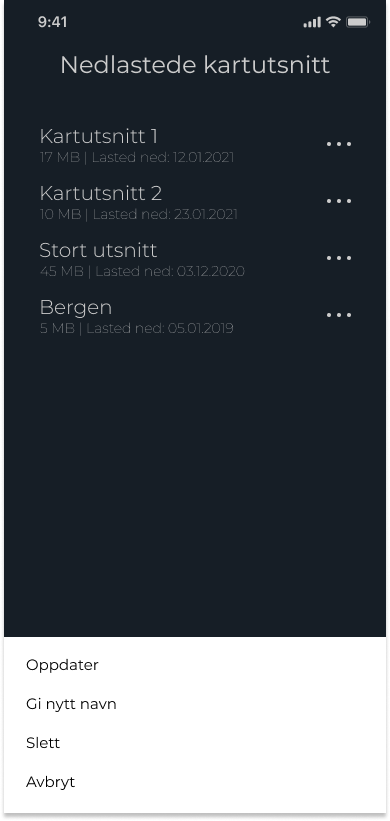
\includegraphics[scale=0.4]{Figurer/Figma/Frame 5 - Nedlastede kartutsnitt meny.png}
\caption{Prototypedesign av side for oversikt over nedlastede kartutsnitt med åpen valgmeny.}
\label{fig:figma-nedlastede-kartutsnitt-med-apen-meny}
\end{figure}
\noindent
Om man trykker på den grønne knappen med et pluss-tegn nede i høyre hjørne på \enquote{Nedlastede kartutsnitt}-siden, vil det navigeres til siden hvor man kan laste ned nye kartutsnitt (figur \ref{fig:figma-laste-ned-kartutsnitt}). Ved å flytte og zoome på kartet slik at det ønskede kartutsnittet kommer innenfor det markerte rektangelet kan man selv velge hvor stort et kartutsnitt skal være. Når man har funnet området på kartet man ønsker å lage et kartutsnitt av trykker man på \enquote{Last ned}-knappen. Ved å trykke på \enquote{Avbryt}-knappen vil man bli tatt tilbake til oversikten over nedlastede kartutsnitt.
\begin{figure}[H]
\centering
\captionsetup{width=.8\linewidth}
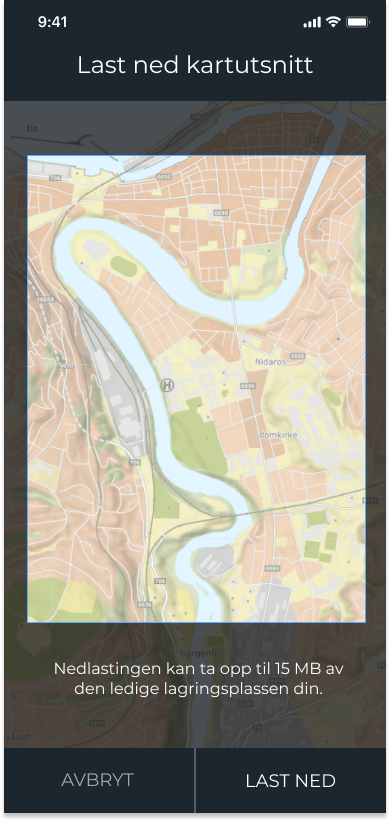
\includegraphics[scale=0.4]{Figurer/Figma/Frame 3 - Last ned kartutsnitt.png}
\caption{Prototypedesign av side for å laste ned nye kartutsnitt.}
\label{fig:figma-laste-ned-kartutsnitt}
\end{figure}

\subsection{Ny oppsynstur}
\subsubsection{Registrering av informasjon}
For å registrere en ny oppsynstur kan man trykke på \enquote{Ny oppsynstur}-knappen på hovedmenyen (figur \ref{fig:valg-av-farger}). Da blir man først tatt til \enquote{Ny oppsynstur}-siden (figur \ref{fig:figma-info-ny-oppsynstur}). Her skal man registrere navnet på deltagerne som er med på oppsynsturen, samt at man kan legge til en beskrivelse for turens formål og baktanke. Når dette er gjort kan man trykke på \enquote{Start oppsynstur}-knappen for å starte selve oppsynsturen. Brukeren vil da bli tatt til kartsiden som er hovedsiden under en oppsynstur.
\begin{figure}[H]
\centering
\captionsetup{width=.8\linewidth}
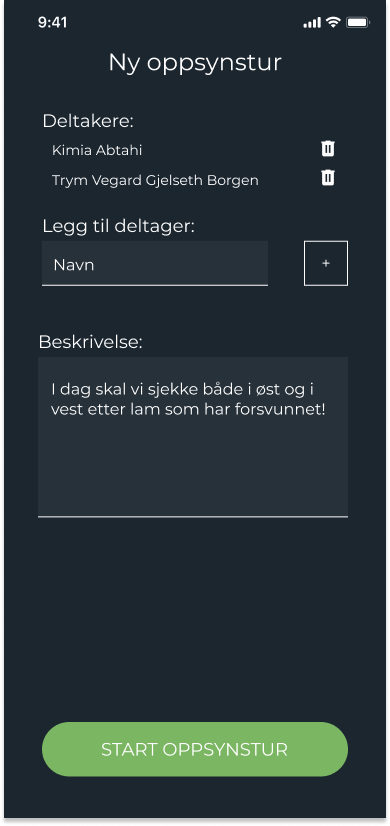
\includegraphics[scale=0.4]{Figurer/Figma/Frame 2 - Ny oppsynstur.png}
\caption{Prototypedesign av side for å registrere informasjon til en ny oppsynstur.}
\label{fig:figma-info-ny-oppsynstur}
\end{figure}

\subsubsection{Kart}
Kartsiden (figur \ref{fig:figma-kart}) i applikasjonen er, som nevnt tidligere, siden som blir mest brukt under en oppsynstur. Kartsiden viser ved hjelp av en blå sirkel hvor man befinner seg på kartet, mens den blå streken viser hvor man har gått.
\begin{figure}[H]
\centering
\captionsetup{width=.8\linewidth}
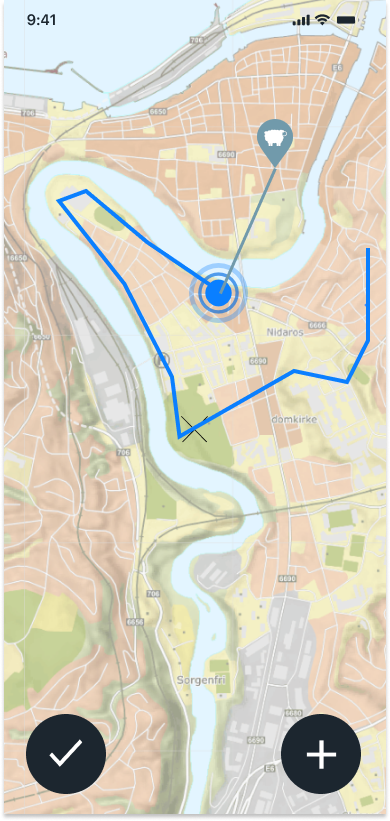
\includegraphics[scale=0.4]{Figurer/Figma/Frame 2.1 - Oppsynstur-kart.png}
\caption{Prototypedesign av side for kart.}
\label{fig:figma-kart}
\end{figure}

\subsubsection{Meny i kart}
Ved å trykke på pluss-knappen nede i høyre hjørne åpnes valgmenyen for å legge til en ny registrering (figur \ref{fig:figma-kart-apen-meny}). Her kan man velge mellom (fra øverst til nederst) å legge til en registrering for en observasjon av en saueflokk, rovdyr, en eller flere døde sauer og en eller flere skadde sauer. Når en registrering har blitt fullført legges det til to ny elementer på kartsiden:
\begin{itemize}
    \item Et merke som viser hvilken type registrering som har blitt utført (Død sau, rovdyr etc.). Dette merket blir da plassert på posisjonen hvor observasjonen ble gjort.
    \item En linje som peker fra hvor observasjonen ble gjort fra og til merket.
\end{itemize}

\noindent
På den måten kan brukeren i etterkant av en oppsyntur vite både hvor eventuelle sauer har blitt observert i tillegg til hvor de ble observert fra. 

\begin{figure}[H]
\centering
\captionsetup{width=.8\linewidth}
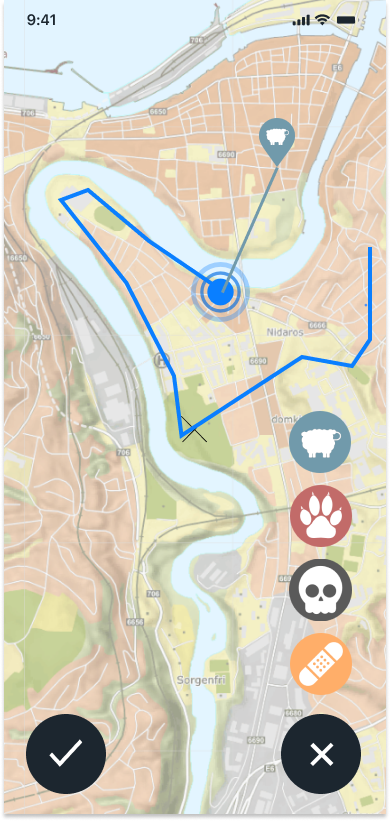
\includegraphics[scale=0.4]{Figurer/Figma/Frame 2.1 - Oppsynstur-kart-apen-meny.png}
\caption{Prototypedesign av side for kart med åpen valgmeny.}
\label{fig:figma-kart-apen-meny}
\end{figure}

\subsection{Fullføre oppsynstur}
For å fullføre en oppsynstur trykkes det på fullfør-knappen nede i venstre hjørne på kartsiden (figur \ref{fig:figma-kart}). Ved å gjøre dette vil applikasjonen navigere til \enquote{Oppsummering}-siden (figur \ref{fig:figma-oppsummering}). Oppsummeringssiden viser generell informasjon om turen, samt hvor brukeren har gått og hvilke observasjoner som har blitt gjort. Her er det også mulig å legge til en kommentar før det trykkes fullfør og oppsynsturen blir lagret.
\begin{figure}[H]
\centering
\captionsetup{width=.8\linewidth}
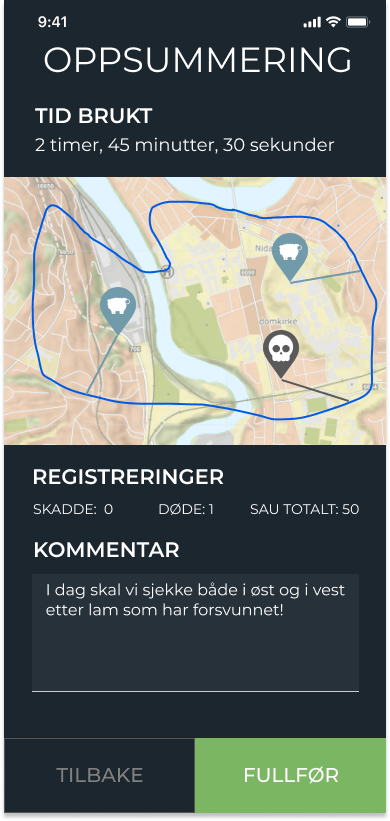
\includegraphics[scale=0.4]{Figurer/Figma/Frame 2.3 - Oppsummering oppsynstur.png}
\caption{Prototypedesign av side for oppsummering av en oppsynstur.}
\label{fig:figma-oppsummering}
\end{figure}

\subsection{Legge til en registrering}
\subsubsection{Registrering av sau} 
\label{subsubsec:registrering av sau}
Grensesnittet for registrering av sau ble nesten ferdig utformet i fordypningsprosjektet og kan leses om i sin helehet der \cite{Abtahi2020TilsynBeite}. Det eneste som har blitt lagt til grensesnittet for registrering av sau siden da er funksjonalitet for å legge til øremerker. Figur \ref{fig:figma-legge-til-oremerker} viser den nye siden for registrering av øremerker. Listen er en flervalgsliste som inneholder fargen på merket og navnet på bonden som øremerkene tilhører.
\begin{figure}[H]
\centering
\captionsetup{width=.8\linewidth}
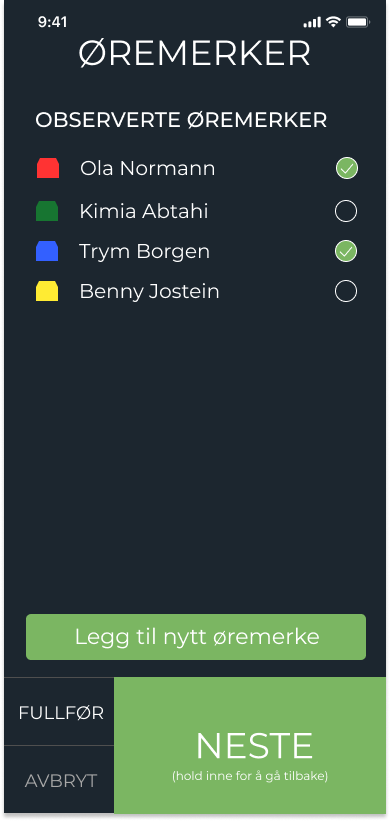
\includegraphics[scale=0.4]{Figurer/Figma/Frame 2.2.2 - oremerker.png}
\caption{Prototypedesign av side for å legge til et øremerker i en registrering.}
\label{fig:figma-legge-til-oremerker}
\end{figure}
\noindent
For å legge til et nytt øremerke i lista trykker man på \enquote{Legg til nytt øremerke}-knappen (figur \ref{fig:figma-legge-til-oremerker}). Det vil åpne et annet grensesnitt hvor man kan registrere et nytt øremerke (figur \ref{fig:figma-registrere-nytt-oremerke}). I \enquote{Eier}-feltet skriver mann inn navnet på bonden som eier sauene som bærer det nye øremerket. Fargen(e) på merket legges til i grensesnittet under. Mattilsynets regler for øremerker \cite{Mattilsynet2013remerkingSmafe} sier at alle farer er tillatt, med unntak av hvit, lilla og lakserød. Etter en undersøkelse av flere kilder \cite{remerker, GolSA, NannestadGeit} for beitelag og saumerker virker det som om de fleste øremerker består av enten 1 eller 2 farger. Den foreslåtte løsningen tillatter at det legges til maks 2 farger per øremerke. Fargevelgeren gjør det mulig å velge mellom alle mulige fargekombinasjoner som måtte være ønskelig for brukeren.
\begin{figure}[H]
\centering
\captionsetup{width=.8\linewidth}
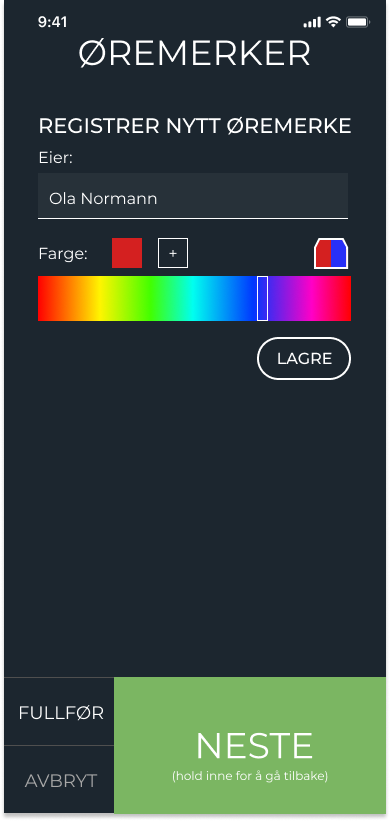
\includegraphics[scale=0.4]{Figurer/Figma/Frame 2.2.2 - lag-oremerke.png}
\caption{Prototypedesign av side for å registrere et nytt øremerke.}
\label{fig:figma-registrere-nytt-oremerke}
\end{figure}
\noindent
Oppsummeringssiden (figur \ref{fig:figma-sau-oppsummering}) for registrering av sau har også blitt oppdatert for å vise hvilke øremerker som har blitt valgt under en registrering. Ellers er den identisk med oppsummeringssiden som ble laget under fordypningsprosjektet.

\begin{figure}[H]
\centering
\captionsetup{width=.8\linewidth}
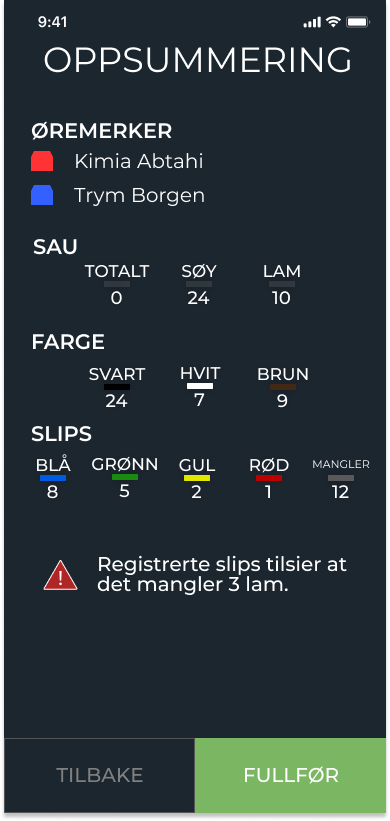
\includegraphics[scale=0.4]{Figurer/Figma/Frame 2.2.5 - Oppsummering.png}
\caption{Prototypedesign av side for oppsummering for registrering av sau.}
\label{fig:figma-sau-oppsummering}
\end{figure}

\subsubsection{Registrering av rovdyr}
For å registrere et rovdyr trykker man på det røde ikonet i valgmenyen med et poteavtrykk (figur \ref{fig:figma-kart-apen-meny}). Herfra blir man tatt til registreringssiden for rovdyr (figur \ref{fig:figma-registrer-rovdyr}). Rovdyrene man kan legge til er forhåndsbestemt og kan enkelt velges fra nedtrekkslisten. Valget av rovdyr begrunnes i underkapittel \ref{sub:rovdyr} \nameref{sub:rovdyr}. I tillegg til dette kan man legge til en kommentar om man ønsker. Man kan fullføre regitereringen ved å trykke på \enquote{Fullfør}-knappen. Registreringen kan også avbrytes ved å trykke på \enquote{Tilbake}-knappen som tar brukeren tilbake til kartsiden.
\begin{figure}[H]
\centering
\captionsetup{width=.8\linewidth}
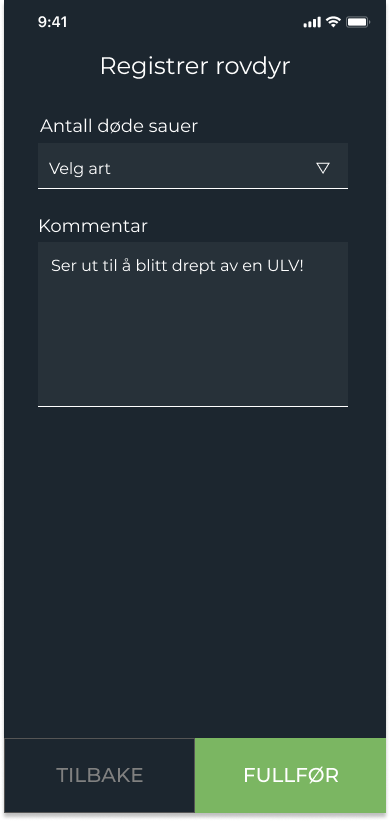
\includegraphics[scale=0.4]{Figurer/Figma/Frame 2.2c.1 - Registrer rovdyr.png}
\caption{Prototypedesign av side for registrering av rovdyr.}
\label{fig:figma-registrer-rovdyr}
\end{figure}

\subsubsection{Registrering av død sau}
For å registrere død sau trykker man på den mørkegrå knappen med et dødninghode i valgmenyen på kartsiden (figur \ref{fig:figma-kart-apen-meny}). Deretter blir man tatt til registreringssiden for døde sauer (figur \ref{fig:figma-registrer-dode-sauer}). Antallet døde sauer man finner på en lokasjon registreres under feltet \enquote{Antall døde sauer}. Man kan også legge til en kommentar om ønskelig. I følge Statsforvalteren skal det ved mistanke om skade på sau som følge av rovdyr tas bilde av kadaveret som knyttes til GPS-koordinater \cite[~s.19]{StatsforvaltereniInnlandet2020InformasjonInnlandet}. Denne informasjonen blir brukt som grunnlag når det søkes om erstatning for tap av sau \cite{2014ForskriftRovvilt, MiljdirektoratetErstatningRovvilt}. Det er derfor lagd design for funksjonalitet som lar brukeren legge til et eller flere bilder som blir lagret sammen med registreringen. Etter at ønsket informasjon er fylt ut kan man trykke på \enquote{Fullfør}-knappen for å lagre registreringen og gå tilbake til kartsiden. Hvis man ikke ønsker å lagre registreringen kan man trykke på \enquote{Tilbake}-knappen.
\begin{figure}[H]
\centering
\captionsetup{width=.8\linewidth}
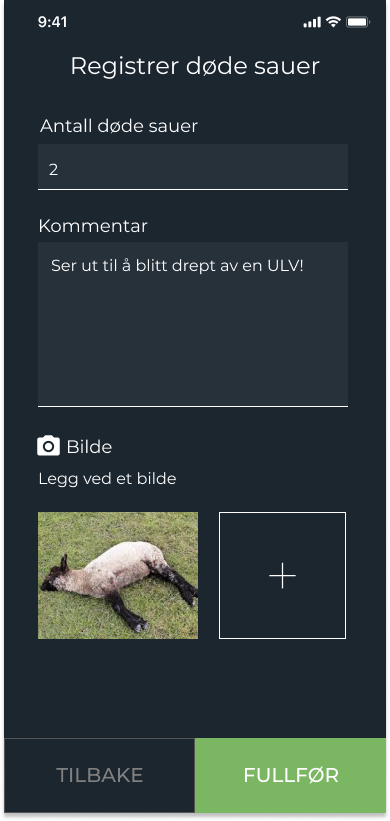
\includegraphics[scale=0.4]{Figurer/Figma/Frame 2.2b.1 - Registrer-dode-sauer.png}
\caption{Prototypedesign av side for registrering av døde sauer.}
\label{fig:figma-registrer-dode-sauer}
\end{figure}

\subsubsection{Registrering av skadet sau}
For å registrere skadet sau trykker man på den gule knappen med et plaster i valgmenyen på kartsiden (figur \ref{fig:figma-kart-apen-meny}). Herfra blir man tatt til siden for registrering av skadet sau (figur \ref{fig:figma-registrer-skadd-sau}). Antall skadde sauer registreres under feltet \enquote{Antall skadde sauer}. Det er også mulig å legge ved en eventuell kommentar. Når registreringen er fullført trykker man på \enquote{Fullfør}-knappen for å lagre registreringen og gå tilbake til kartsiden. Hvis man ønsker å forkaste registreringen kan man trykke på \enquote{Tilbake}-knappen for å gå tilbake til kartsiden uten å lagre.
\begin{figure}[H]
\centering
\captionsetup{width=.8\linewidth}
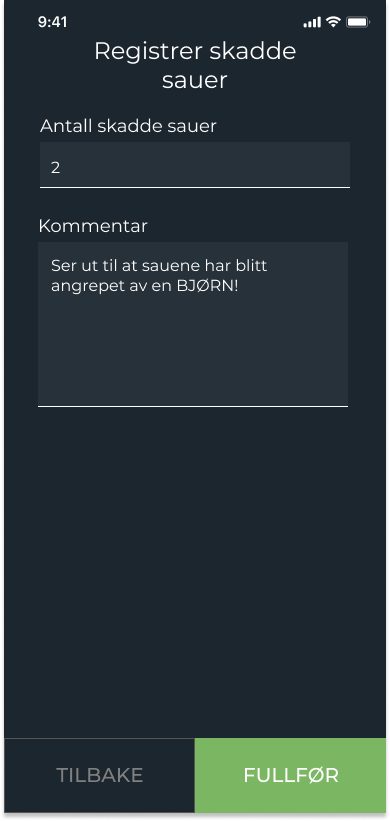
\includegraphics[scale=0.4  ]{Figurer/Figma/Frame 2.2a.1 - Registrer-skadde-sauer.png}
\caption{Prototypedesign av side for registrering av skadd sauer.}
\label{fig:figma-registrer-skadd-sau}
\end{figure}

\subsection{Lagrede oppsynsturer}
\subsubsection{Liste over lagrede oppsynsturer}
Fra hovedmenyen (figur \ref{fig:valg-av-farger}) kan man navigere seg til en liste over alle lagrede oppsynsturer (figur \ref{fig:figma-oppsynsturer-liste}) ved å trykke på \enquote{Oppsynsturer}-knappen. Hvert element i lista viser én lagret oppsynstur og litt generell informasjon om turen, som hvem som registrerte oppsynsturen, hvor lang tid det tok og hvilken dato den ble utført på. Symbolene nederst i hvert element viser (fra venstre) hvor mange sau som har blitt registrert totalt, hvor mange skadde sau som har blitt registrert, hvor mange døde sau som har blitt registrert og hvor mange rovdyr som har blitt registert.

\begin{figure}[H]
\centering
\captionsetup{width=.8\linewidth}
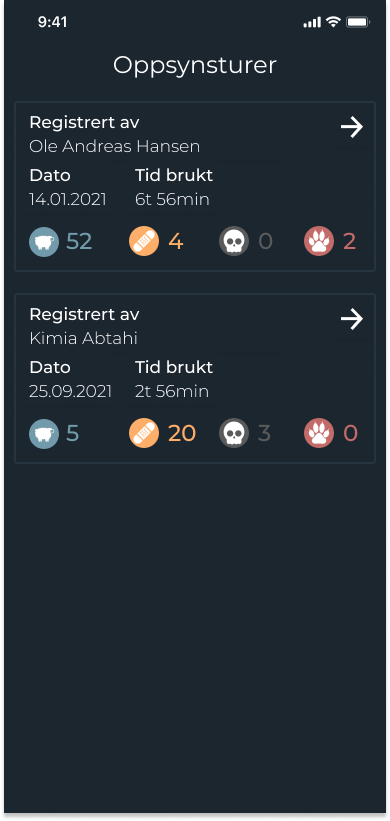
\includegraphics[scale=0.4]{Figurer/Figma/Frame 6 - Oppsynsturer.png}
\caption{Prototypedesign av side for lagrede oppsynsturer.}
\label{fig:figma-oppsynsturer-liste}
\end{figure}

\subsubsection{Oppsummering av en enkelt oppsynstur}
Ved å trykke på pila i et element i lista over oppsynsturer (figur \ref{fig:figma-oppsynsturer-liste}) blir man tatt til siden som viser detaljert informasjon om den valgte oppsynsturen (figur \ref{fig:figma-lagret-oppsynstur}). Siden viser ruta man har gått på kartet, samt alle registreringer som har blitt gjort og hvor de ble gjort fra. Under kartet er fire ekspanderbare elementer som kan åpnes og lukkes for å vise de forskjellige registreringene som har blitt gjort under hver av de fire kategoriene. Ikonet med tallet på siden viser det totale antallet sau, skadde sau, døde sau eller rovdyr som har blitt registrert under kategorien. Ved å trykke på pila til høyre i boksen ekspanderes lista, og alle registreringer som er gjort innenfor den valgte kategorien vises med all registert informasjon.
\begin{figure}[H]
\centering
\captionsetup{width=.8\linewidth}
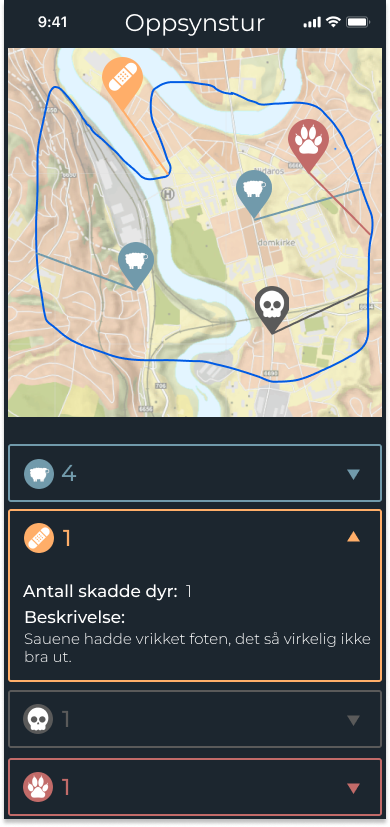
\includegraphics[scale=0.4]{Figurer/Figma/Frame 7 - Oppsynstur-oppsummering.png}
\caption{Prototypedesign av side for oppsummering av en lagret oppsynstur som viser registreringer for skadet sau.}
\label{fig:figma-lagret-oppsynstur}
\end{figure}
\noindent
Ettersom at de forskjellige kategoriene inneholder forskjellig informasjon vil elementene inne i de ekspanderbare boksene være ulike fra kategori til kategori. Figur \ref{fig:figma-lagret-oppsynstur2} viser hvordan informasjonen inne i den ekspanderte boksen for registrering av en saueflokk ser ut.
\begin{figure}[H]
\centering
\captionsetup{width=.8\linewidth}
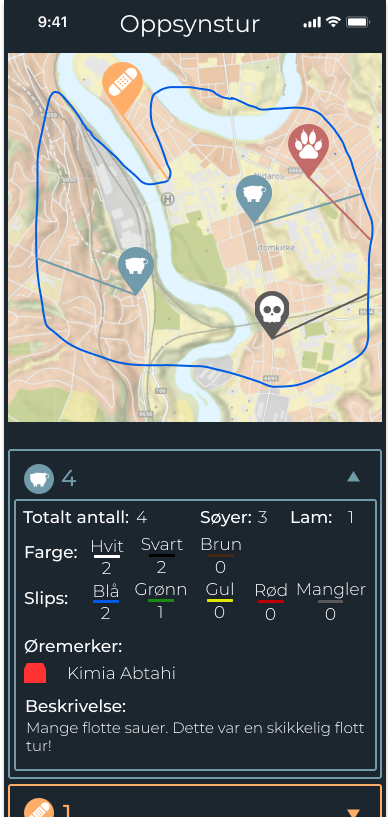
\includegraphics[scale=0.4]{Figurer/Figma/Frame 7 - Oppsynstur-oppsummering2.png}
\caption{Prototypedesign av side for oppsummering av en lagret oppsynstur som viser registreringer for en saueflokk.}
\label{fig:figma-lagret-oppsynstur2}
\end{figure}
\chapter{Implementasjon}
Dette kapittelet tar for seg resultatet av utformingen av applikasjonen, hvordan tilstandshåndteringen er implementert og hvordan applikasjonen samhandler med backendløsningen i Firebase. Det ble tidlig besluttet å ikke utføre brukertester på prototypedesignet som ble laget i Figma. Årsaken til dette var at det ble sett på som lite hensiktsmessig da applikasjonen i stor grad ville ta i bruk funksjonalitet som ikke kunne testes i prototypeverktøyet. Her tenkes det spesifikt på bruk av kart og GPS, som er en av hovedfunksjonalitetene i applikasjonen. Implementasjonen ble derfor startet på direkte etter at prototypedesignet i Figma var ferdigstilt.

\section{Utforming}
Dette underkapittelet tar for seg resultatene av utformingen av selve applikasjonen. De forskjellige brukergrensesnitt-sidene er utviklet i henhold til prototype-designet (se kapittel \ref{cha:Design} \nameref{cha:Design}) som ble laget i Figma under design-fasen av prosjektet. Alle figurene vist i dette underkapittelet er skjermbilder hentet fra iOS-versjonen av applikasjonen på iPhone 12 Pro. 

\subsection{Login}
Login-siden er den eneste siden som ikke har et prototype-design laget i Figma. Dette er fordi det først var tenkt å bruke et ferdiglaget verktøy for implementering av brukergrensesnitt for innloggingsider i Angular med Firebase kalt FirebaseUI-Angular \cite{jenniRaphaelJenniFirebaseUIAngular2021}. Grunnet problemer under implementasjonen av FirebaseUI-Angular ble denne idéen skrinlagt og en standard login-side med bruk av e-post og passord ble utformet isteden. Logikken og funksjonaliteten rundt selve innloggingen blir forklart i underkapittel \ref{sub:backend-login} \nameref{sub:backend-login}.
\begin{figure}[H]
\centering
\captionsetup{width=.8\linewidth}
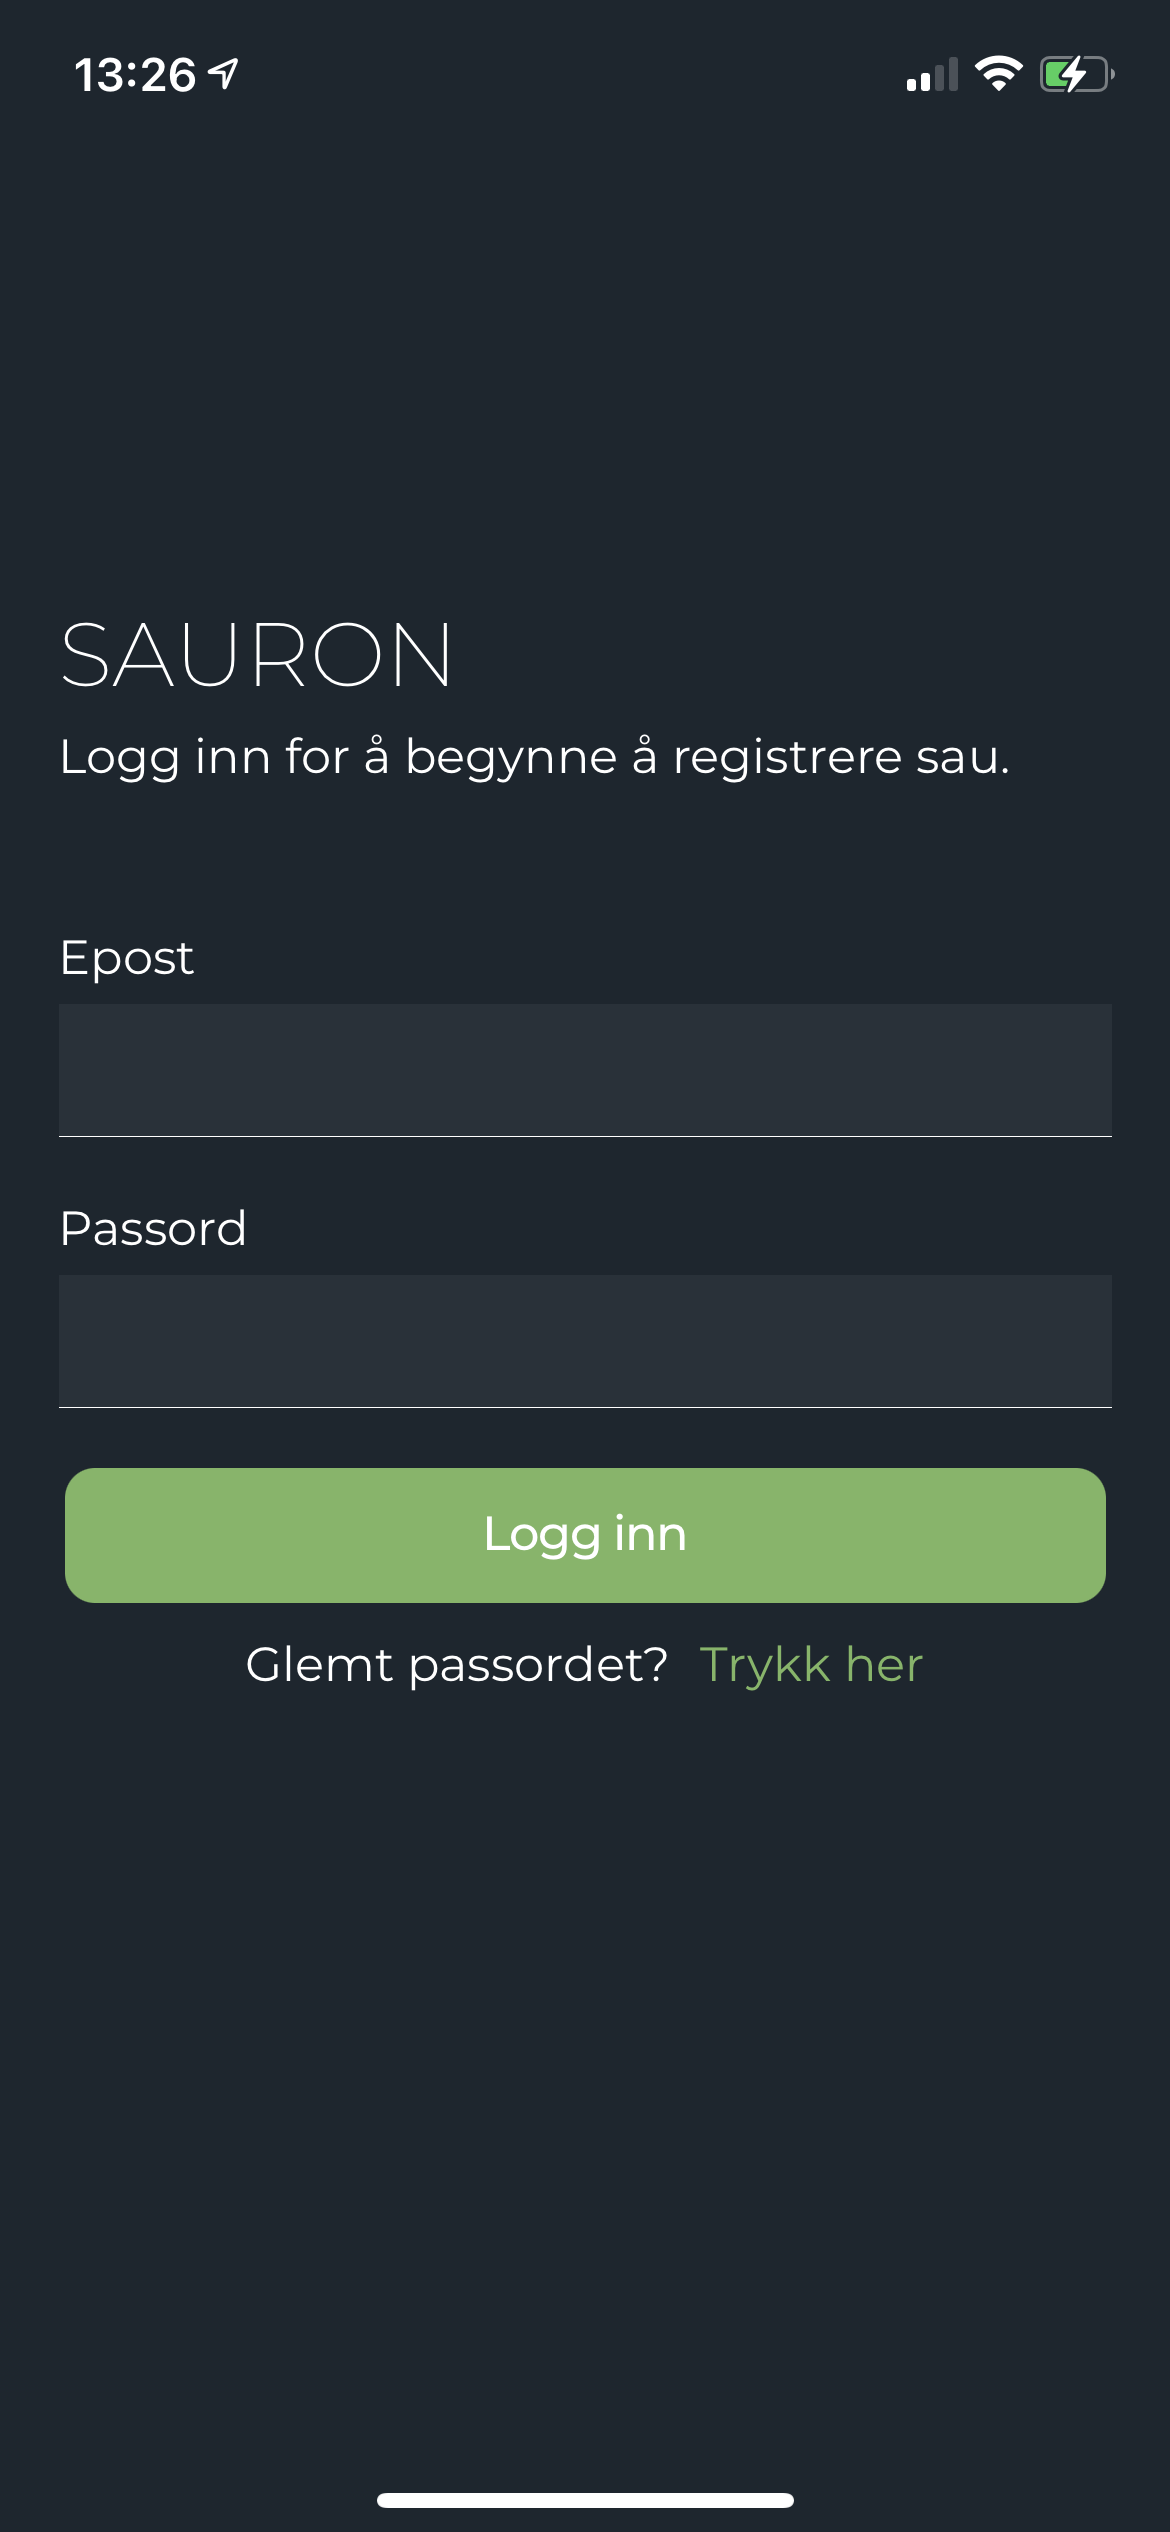
\includegraphics[scale=0.4]{Figurer/skjermbilder/login.png}
\caption{Login-side for applikasjonen.}
\label{fig:login}
\end{figure}

\subsection{Nedlasting av kartutsnitt}
\subsubsection{Oversikt over nedlastede kartutsnitt}
Siden som viser en liste over alle nedlastede kartutsnitt er utformet i henhold til design-prototypen. Det samme gjelder for valgmenyen som kommer opp hvis man trykker på de tre prikkene til høyre for hvert liste-element. Under intern testing av grensesnittet viste det seg at det var behov for en navigasjonsknapp for å kunne navigere tilbake til hovedmenyen om ønskelig. Denne har blitt implementert i form av en pil som peker til venstre opp i venstre hjørne av grensesnittet (se figur \ref{fig:nedlastede-kartutsnitt}). 
\begin{figure}[H]
  \centering
  \begin{minipage}[b]{0.4\textwidth}
    \centering
    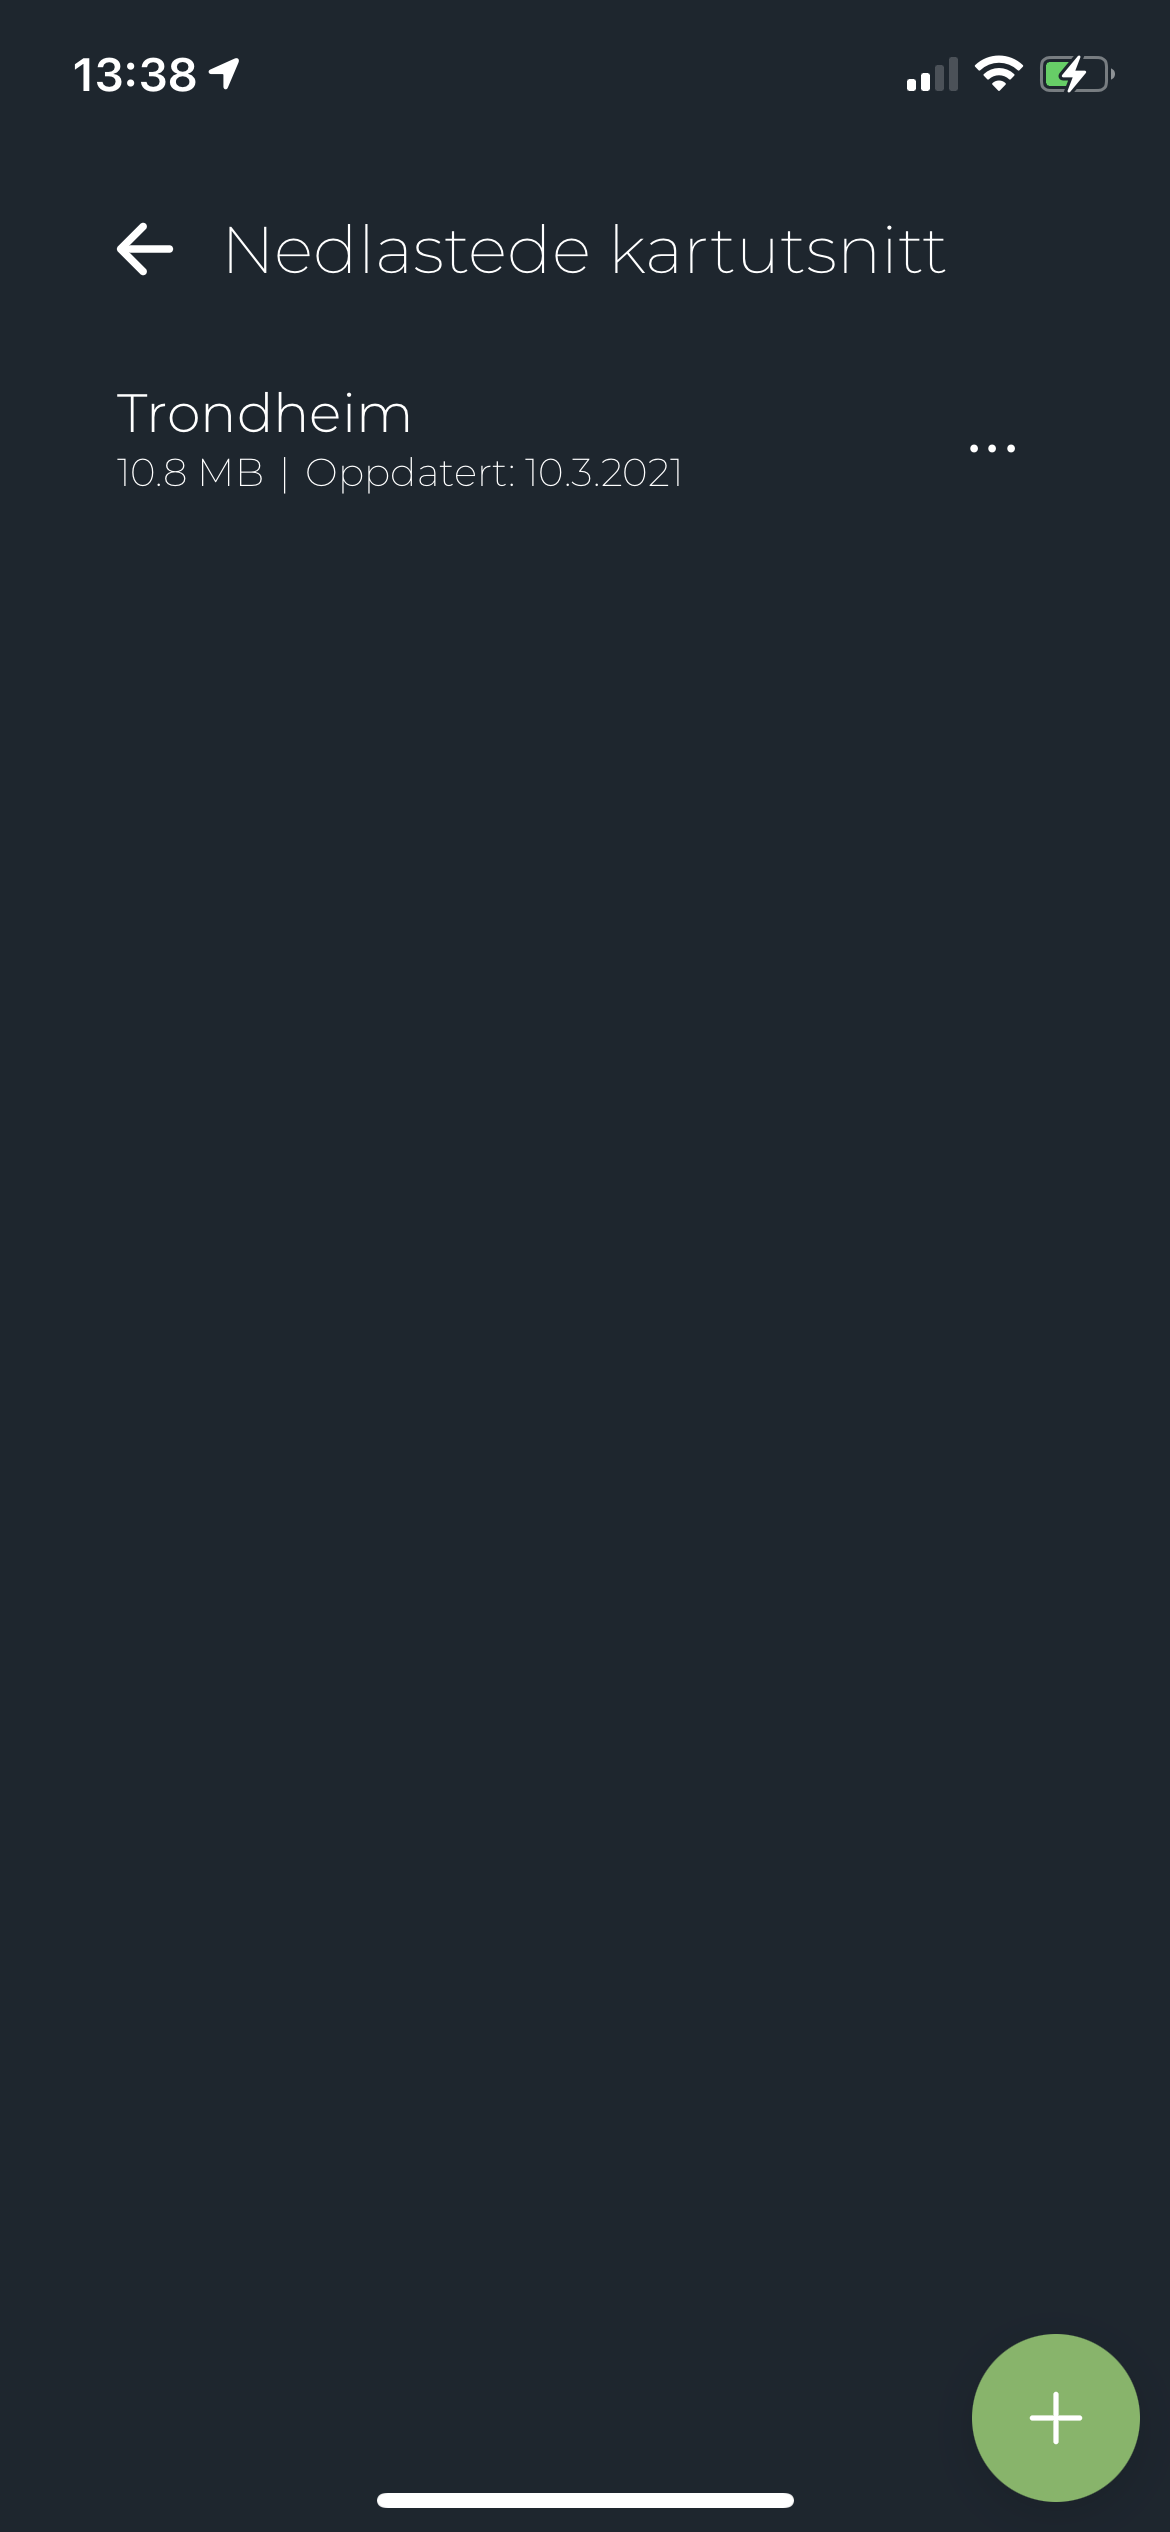
\includegraphics[scale=0.4]{Figurer/skjermbilder/nedlastede-kartutsnitt.png}
    \caption{Oversikt over nedlastede kartutsnitt.}
    \label{fig:nedlastede-kartutsnitt}
  \end{minipage}
  \hfill
  \begin{minipage}[b]{0.4\textwidth}
    \centering
    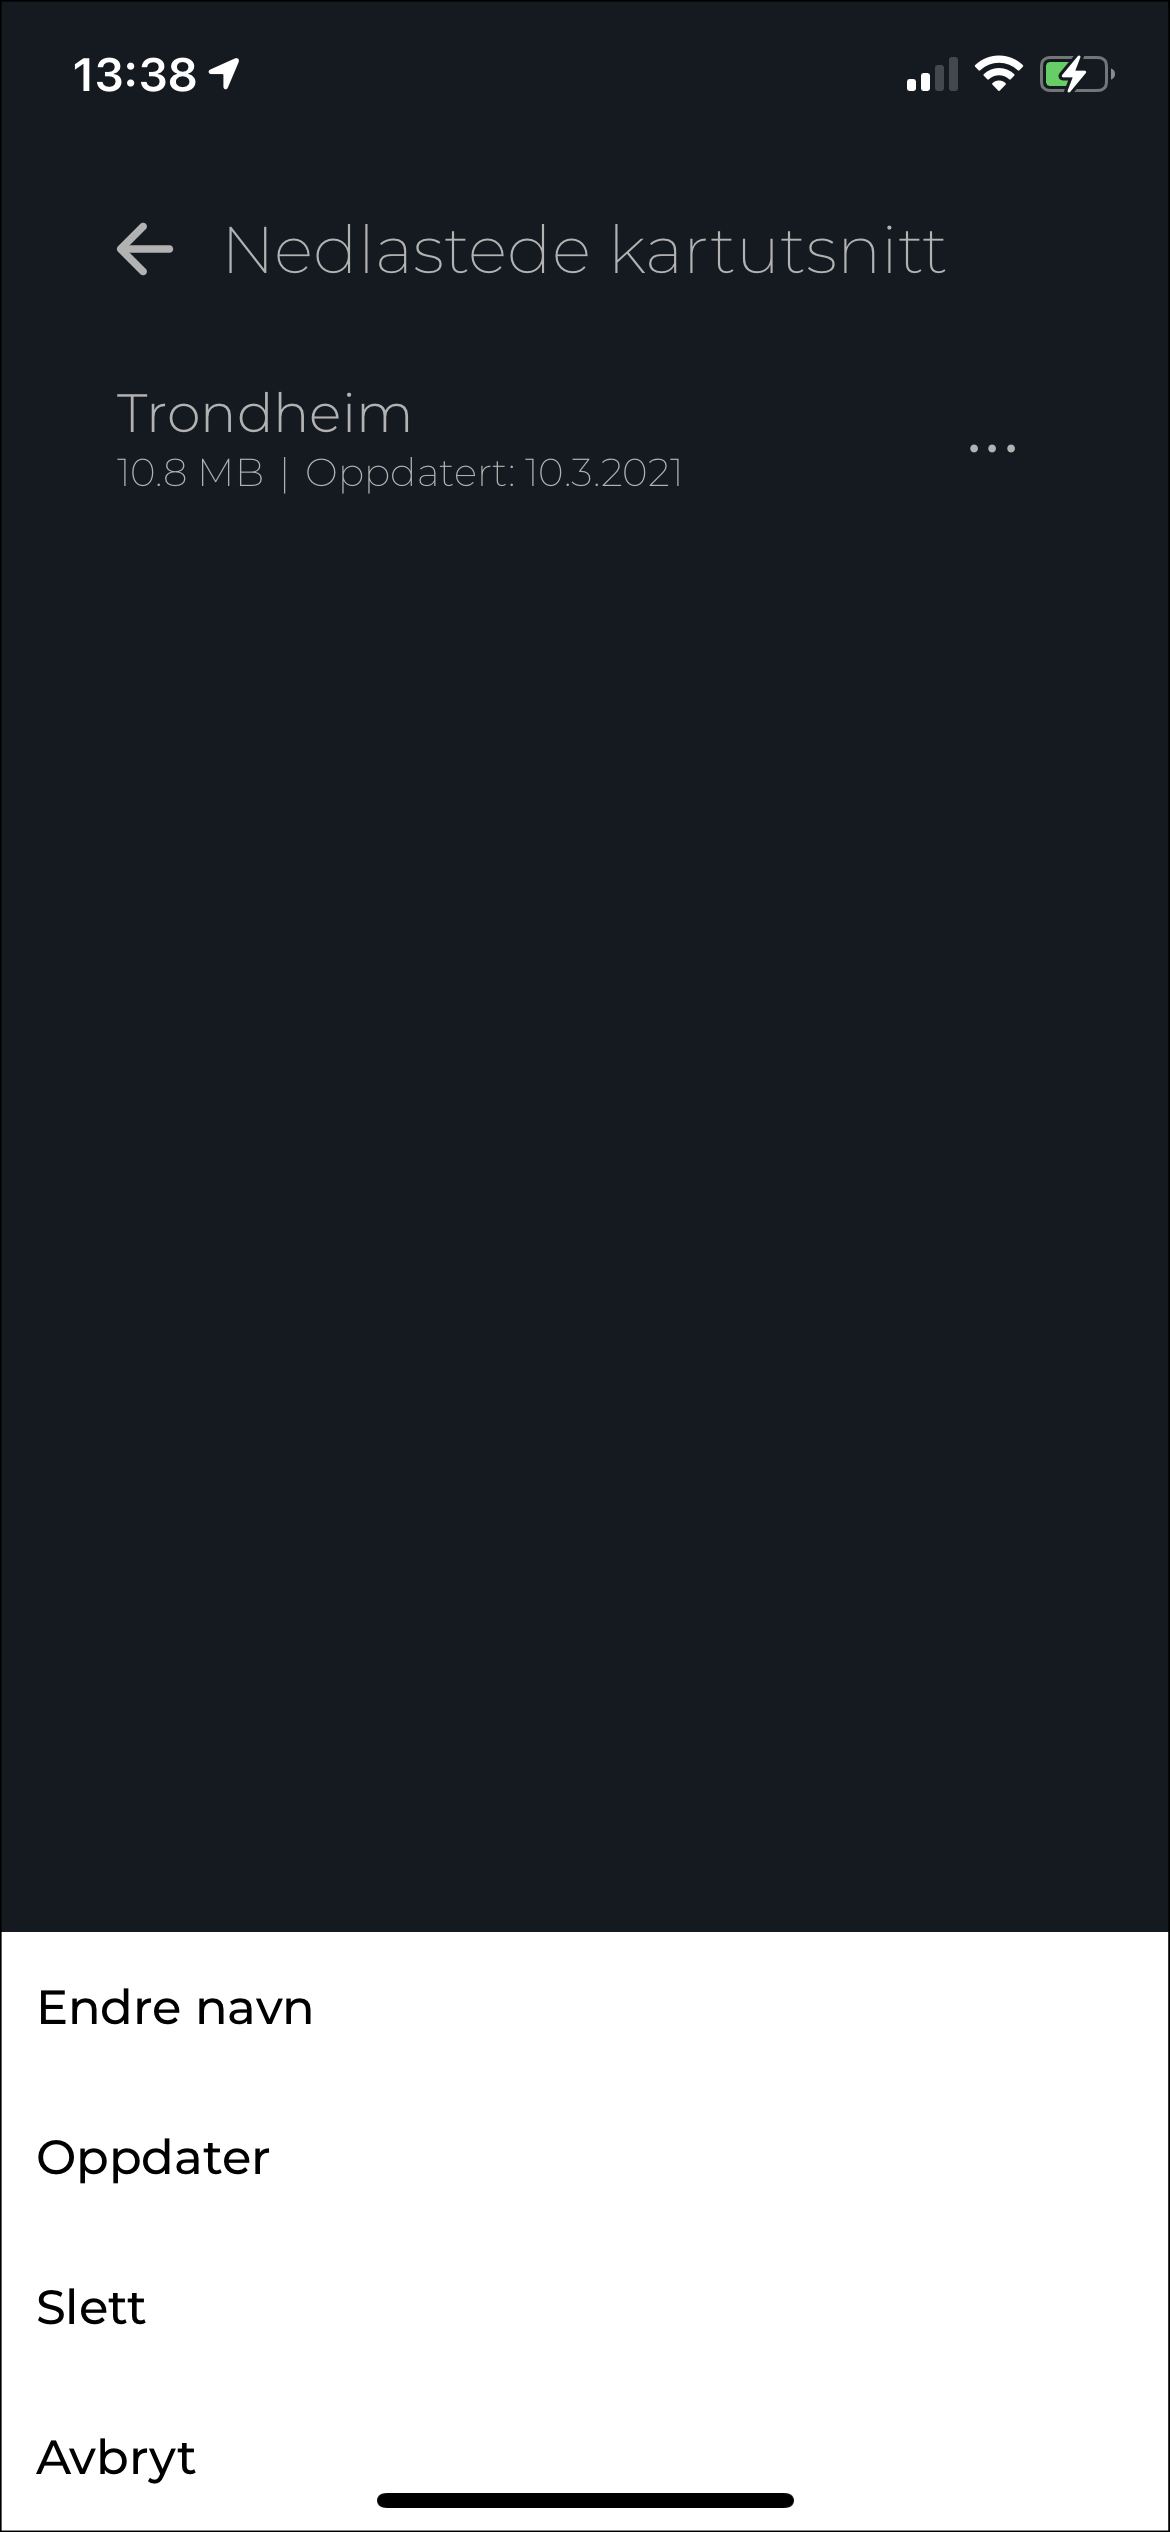
\includegraphics[scale=0.4]{Figurer/skjermbilder/nedlastede-kartutsnitt-apen-meny.png}
    \caption{Valg-meny åpen for et nedlastet kartutsnitt.}
    \label{fig:nedlastede-kartutsnitt-apen-meny}
  \end{minipage}
\end{figure}

\subsubsection{Laste ned nytt kartutsnitt}
For å laste ned et nytt kartutsnitt trykker man på den grønne pluss-knappen vist i figur \ref{fig:nedlastede-kartutsnitt}. Figur \ref{fig:last-ned-nytt-kartutsnitt} viser grensesnittet hvor man velger hvor kartutsnittet skal tas fra og hvor stort det skal være. Her velger man kartutsnittet ved å dra kartet slik at området man ønsker skal komme med havner innenfor det markerte området. Man kan zoome inn og ut for å minske eller øke arealet som det skal lages kartutsnitt av. Grensesnittet er laget helt i henhold til design-prototypen med unntak av pilen for navigering tilbake til siden for nedlastede kartutsnitt. Når man trykker på "Last ned"-knappen starter nedlastingen og man blir tatt tilbake til siden med nedlastede kartutsnitt. Progresjon for nedlastingen vises i grensesnittet i form av en loading-bar som fylles opp til toppen etterhvert som nedlastingen blir ferdig. Når nedlastingen er ferdig vil grensesnittet vise størrelsen på nedlastingen og dato den ble lastet ned. Dette var funksjonalitet som ble designet og implementert etter intern testing da det viste seg at det var behov for en visuell indikator på at kartutsnittet lastes og progresjonen for nedlastingen.
\begin{figure}[H]
  \centering
  \begin{minipage}[b]{0.4\textwidth}
    \centering
    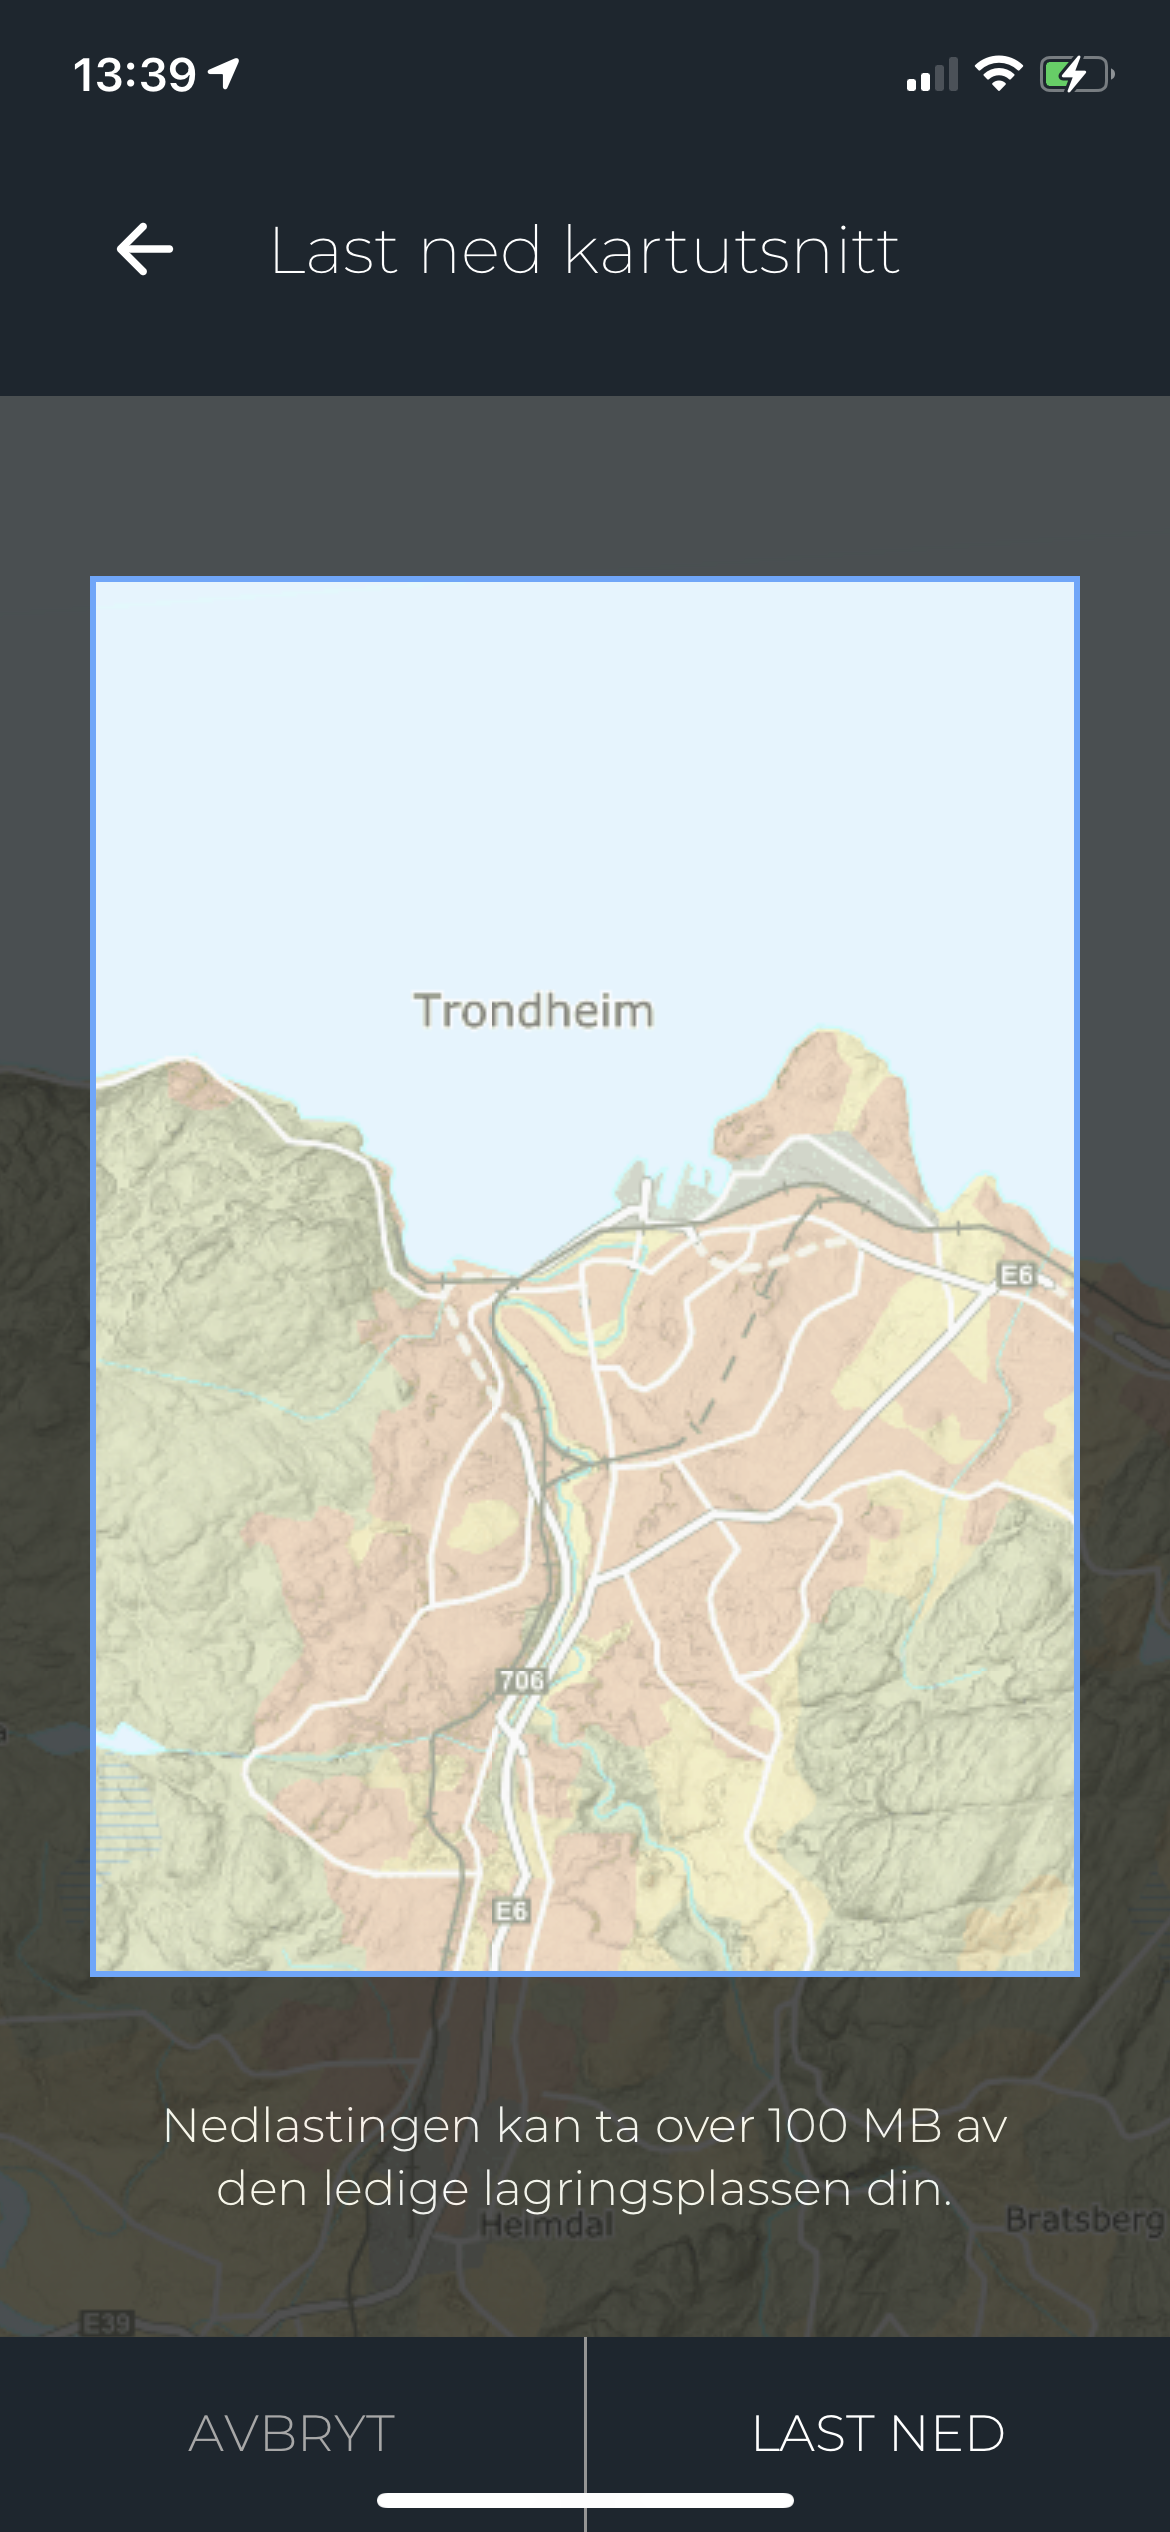
\includegraphics[scale=0.4]{Figurer/skjermbilder/last-ned-nytt-kartutsnitt.png}
    \caption{Side for å laste ned et valg kartutsnitt.}
    \label{fig:last-ned-nytt-kartutsnitt}
  \end{minipage}
  \hfill
  \begin{minipage}[b]{0.4\textwidth}
    \centering
    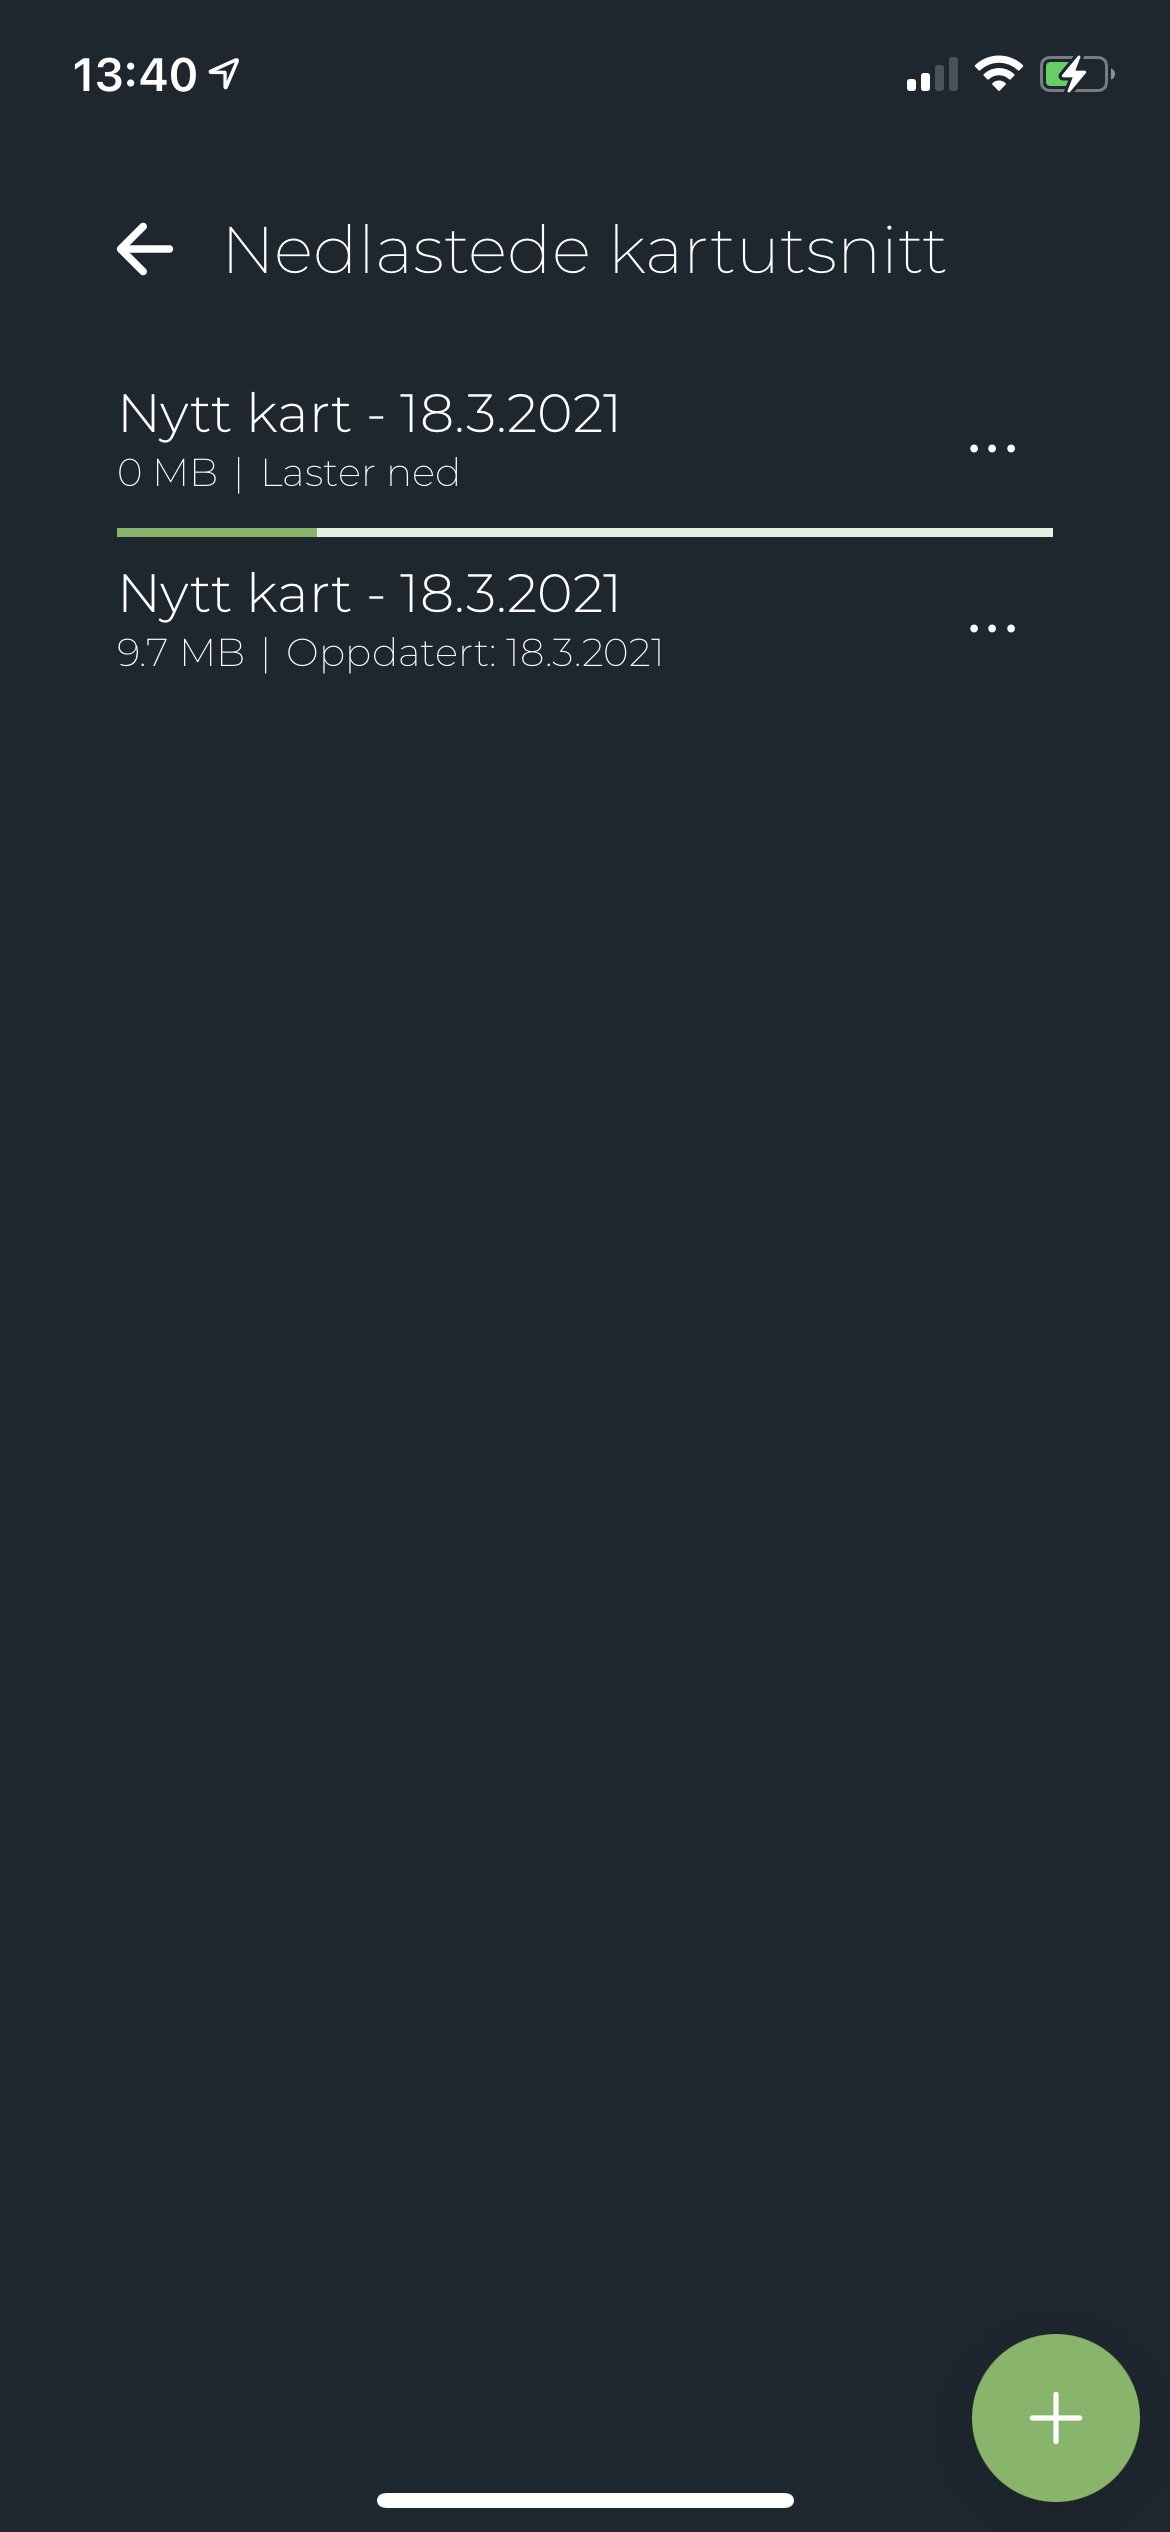
\includegraphics[scale=0.4]{Figurer/skjermbilder/nedlasting-av-nytt-kartutsnitt.png}
    \caption{Progresjon for nedlasting av nytt kartutsnitt.}
    \label{fig:nedlasting-av-nytt-kartutsnitt}
  \end{minipage}
\end{figure}

\noindent
For å laste ned et kartutsnitt brukes cache-tjenesten til Geonorge i form av \textit{opencache}-endepunktene. Cache-tjenestene bygger på underliggende \acrshort{wms}-tjenester, noe som gjør dem svært brukbare i webapplikasjoner \cite{GeoNorgeLeaflet}. Kartet er lagret på tjeneren i form av fliser. Med dette menes det at kartet er delt inn i rektangulære bilder med ulikt detaljnivå basert på hvor zoomet inn man er. For å få tak i en bestemt flis må man oppgi x- og y-koordinaten til flisen, samt zoom-nivå. Et eksempel på et kall til tjenesten er:
\url{https://opencache.statkart.no/gatekeeper/gk/gk.open_gmaps?layers=norges_grunnkart&zoom=14&x=8665&y=4429}. Her hentes flisen med x-koordinat 8665, y-koordinat 4429 og zoom-nivå 14 ut fra tjeneren.
\begin{figure}[H]
\centering
\captionsetup{width=.8\linewidth}
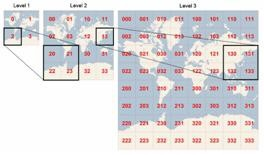
\includegraphics[scale=1.0]{Figurer/Bilder/tilesitiles.jpg}
\caption{Illustrasjon av hvordan kartet er delt inn i fliser.}
\label{fig:map-tiles}
\source{\cite{GeoNorgeLeaflet}}
\end{figure}

\noindent
For at kartet skal fungere uten internett må hver eneste flis for det valgte kartutsnittet lastes ned og lagres på en måte som gjør det mulig å hente ut en bestemt flis basert på x- og y-koordinat og zoom-nivå. Denne prosessen starter med at piksel-koordinatene for øvre venstre hjørne og nedre høyre hjørne for rektangelet som markerer kartutsnittet (se figur \ref{fig:figma-laste-ned-kartutsnitt}) gjøres om det GPS-koordinater. Det kan enkelt gjøres med en innbygd metode i Leaflet kalt containerPointToLatLng({x, y}) \cite{LeafletDom}. Deretter kan GPS-koordinater gjøres om til flis-koordinater med en standardisert metode \cite{SlippyMapTilenames}. Under nedlastingen sendes forespørsler til Cache-tjenesten for å laste ned alle kart-flisene fra øvre venstre til nedre høyre hjørne, for hvert spesifiserte zoom-nivå. For å balansere lasten på tjeneren veksles det mellom å bruke endepunktene opencache.statkart.no, opencache2.statkart.no og opencache3.statkart.no.
\newline

\noindent
For at Lealet skal klare å hente ut korrekt kart-flis fra det lokale filsystemet på mobiltelefonen, må kartflisene lagres på en måte som gir en URI lik den som benyttes når kart-flisene hentes direkte fra tjeneren. Figur \ref{fig:kartutsnitt-lagring} viser hvordan denne filstrukturen er delt opp. For å hente ut kart-flisen spesifisert i figuren bruker Leaflet URI-en \url{maps/421-A3-AD1/mapTiles/14/8665/4429/mapTile.b64}. En metadata-fil lagres også sammen med kart-flisene med informasjon som tilhører det nedlastede kartutsnittet. Metadata som lagres om kartet er kartutsnittets navn, størrelse (i bytes), nedlastingsdato og lokasjon. Denne metadata-filen brukes for å vise fram nyttig informasjon til brukeren, men også for å utføre intern logikk i programmet som for eksempel når et kart skal oppdateres.  

\begin{figure}[H]
\centering
\captionsetup{width=.8\linewidth}
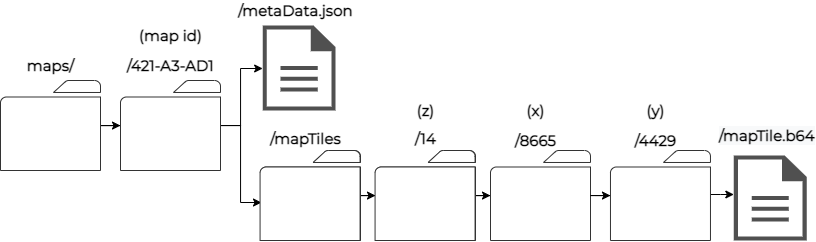
\includegraphics[scale=0.5]{Figurer/diagram/kartutsnitt-lagring.png}
\caption{Eksempel på lagringsstruktur for kartutsnitt med id 423-A3-AD1 og tilhørende kart-flis med koordinater z = 14, x = 8665 og y = 4429.}
\label{fig:kartutsnitt-lagring}
\end{figure}

\subsection{Ny oppsynstur}
\subsubsection{Registrering av informasjon for ny oppsynstur.}
Grensesnittet for registrering av informasjon i sammenheng med en ny oppsynstur har blitt implementert i henhold til design-prototypen. Navnet til brukeren som allerede er logget inn legges til automatisk i listen over deltagere.
\begin{figure}[H]
\centering
\captionsetup{width=.8\linewidth}
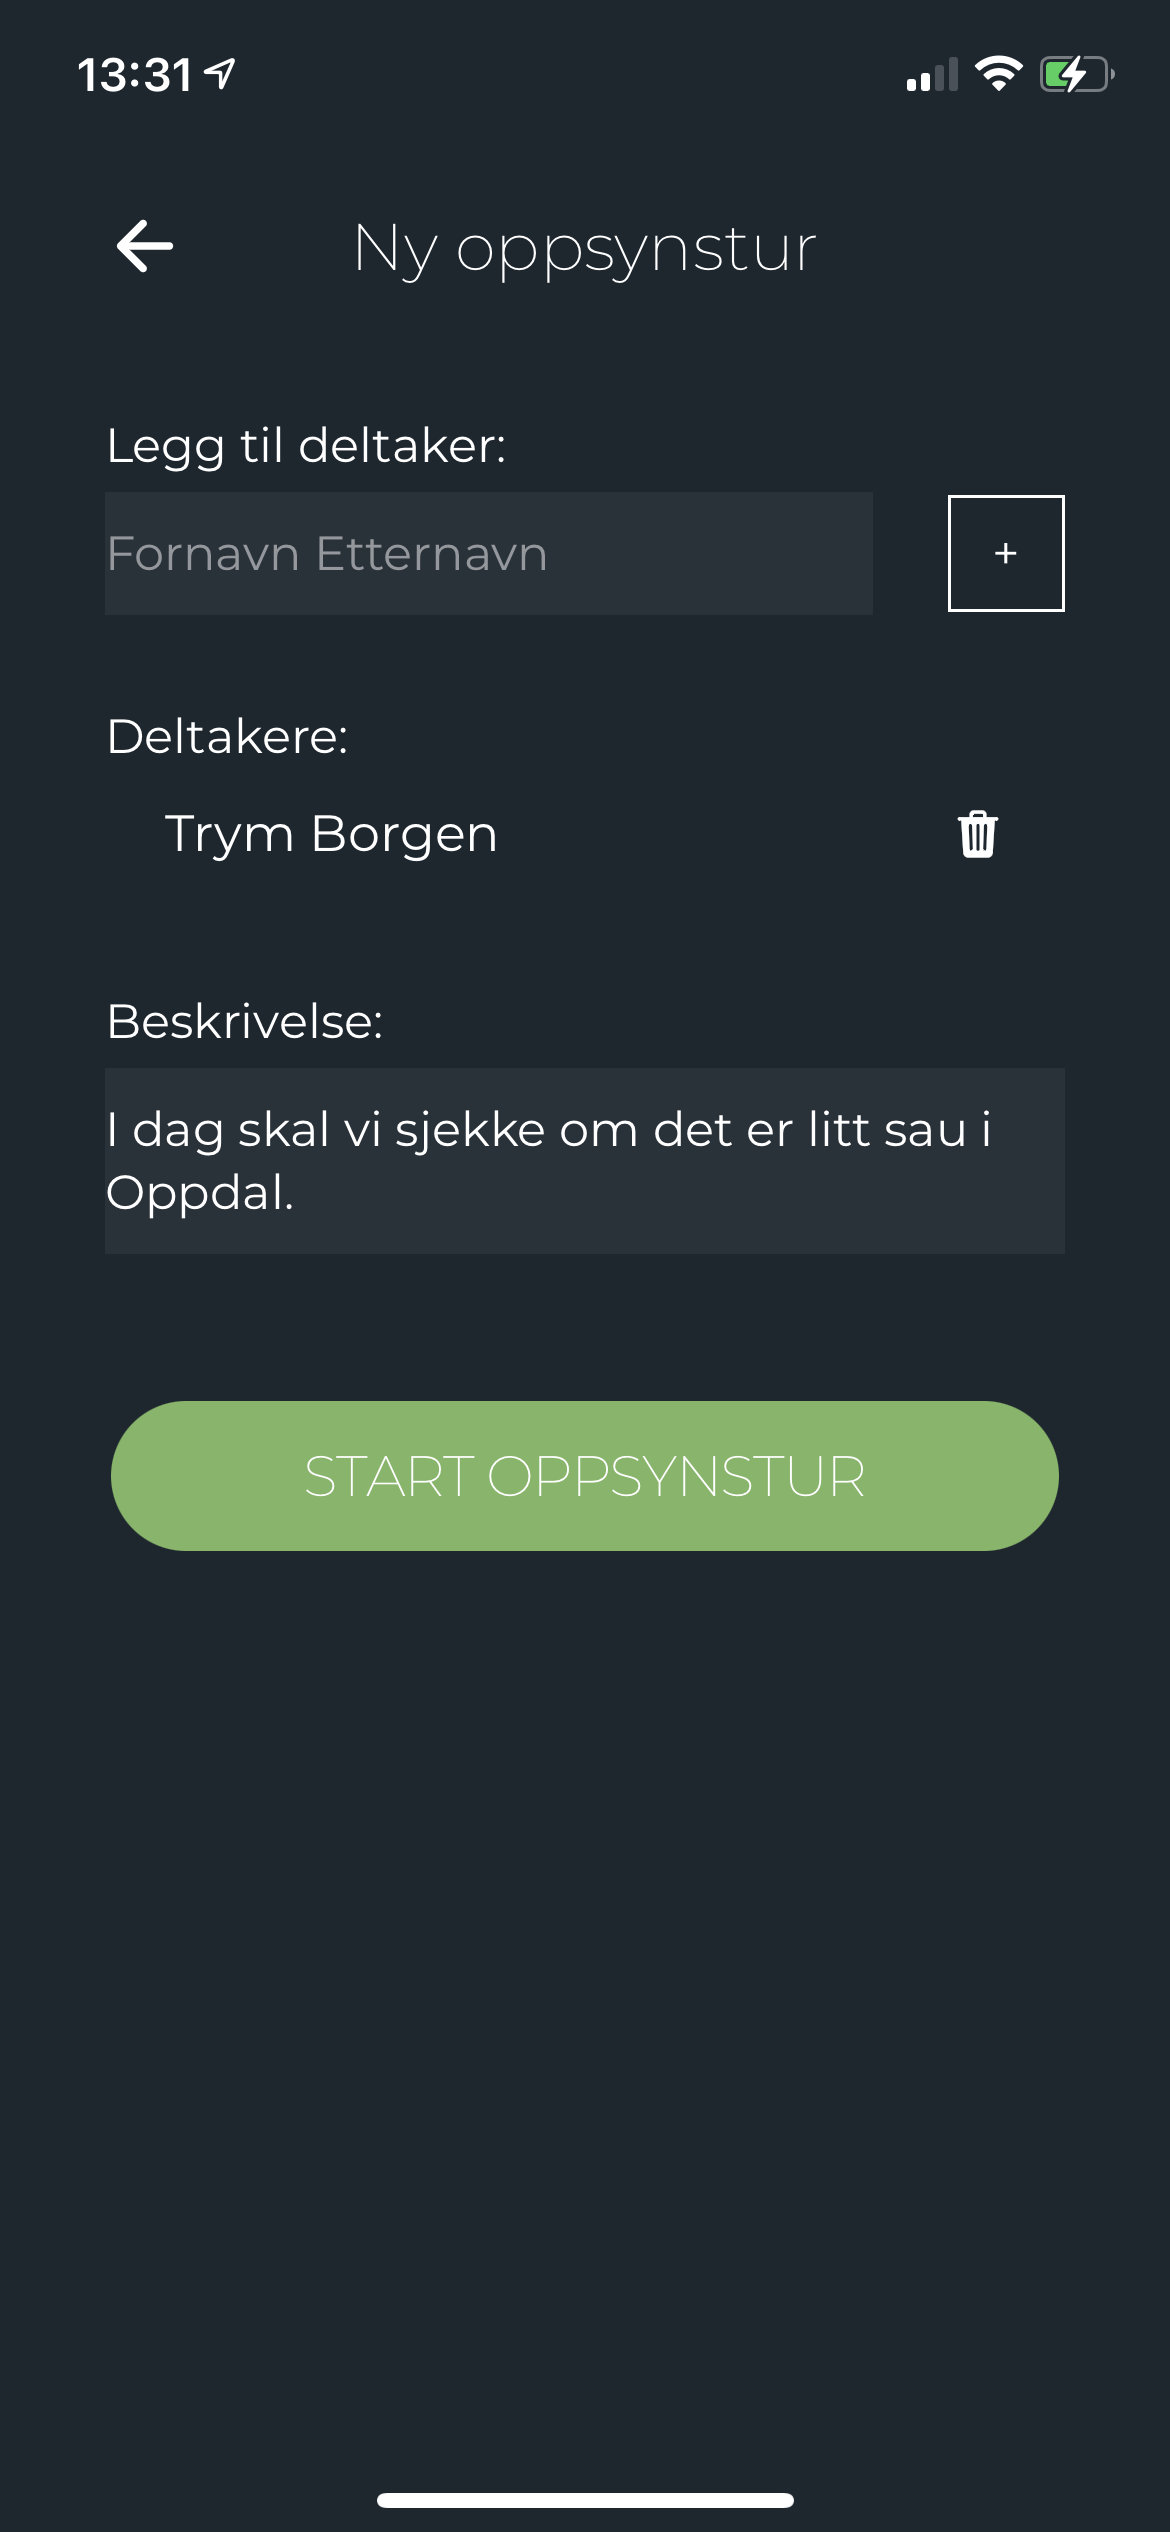
\includegraphics[scale=0.4]{Figurer/skjermbilder/info-oppsynstur.png}
\caption{Implementert grensesnitt for registrering av informasjon før ny oppsynstur.}
\label{fig:info-oppsysntur}
\end{figure}

\subsubsection{Kart}
Kartgrensesnittet som brukes under en en oppsynstur har blitt implementert i henhold til design-prototypen med visse endringer. For det første har størrelsen på symbolene blitt redusert for å gi mer plass til selve kartet. Markøren som viser hvor en registrering blir plassert, som vist i midten av kartet på figur \ref{fig:kart-meny-apen}, har blitt byttet ut med en tydeligere markør som gjør det mulig se sentrum av hva man registrer. Det har også blitt lagt til en knapp nederst i midten av grensesnittet. Denne knappen kan brukes til å sette applikasjonen i strømsparingsmodus som forklares nærmere i underkapittel \ref{sec:bakgrunnsoppdatering-av-gps-lokasjon} \nameref{sec:bakgrunnsoppdatering-av-gps-lokasjon}.

\begin{figure}[H]
  \centering
  \begin{minipage}[b]{0.4\textwidth}
    \centering
    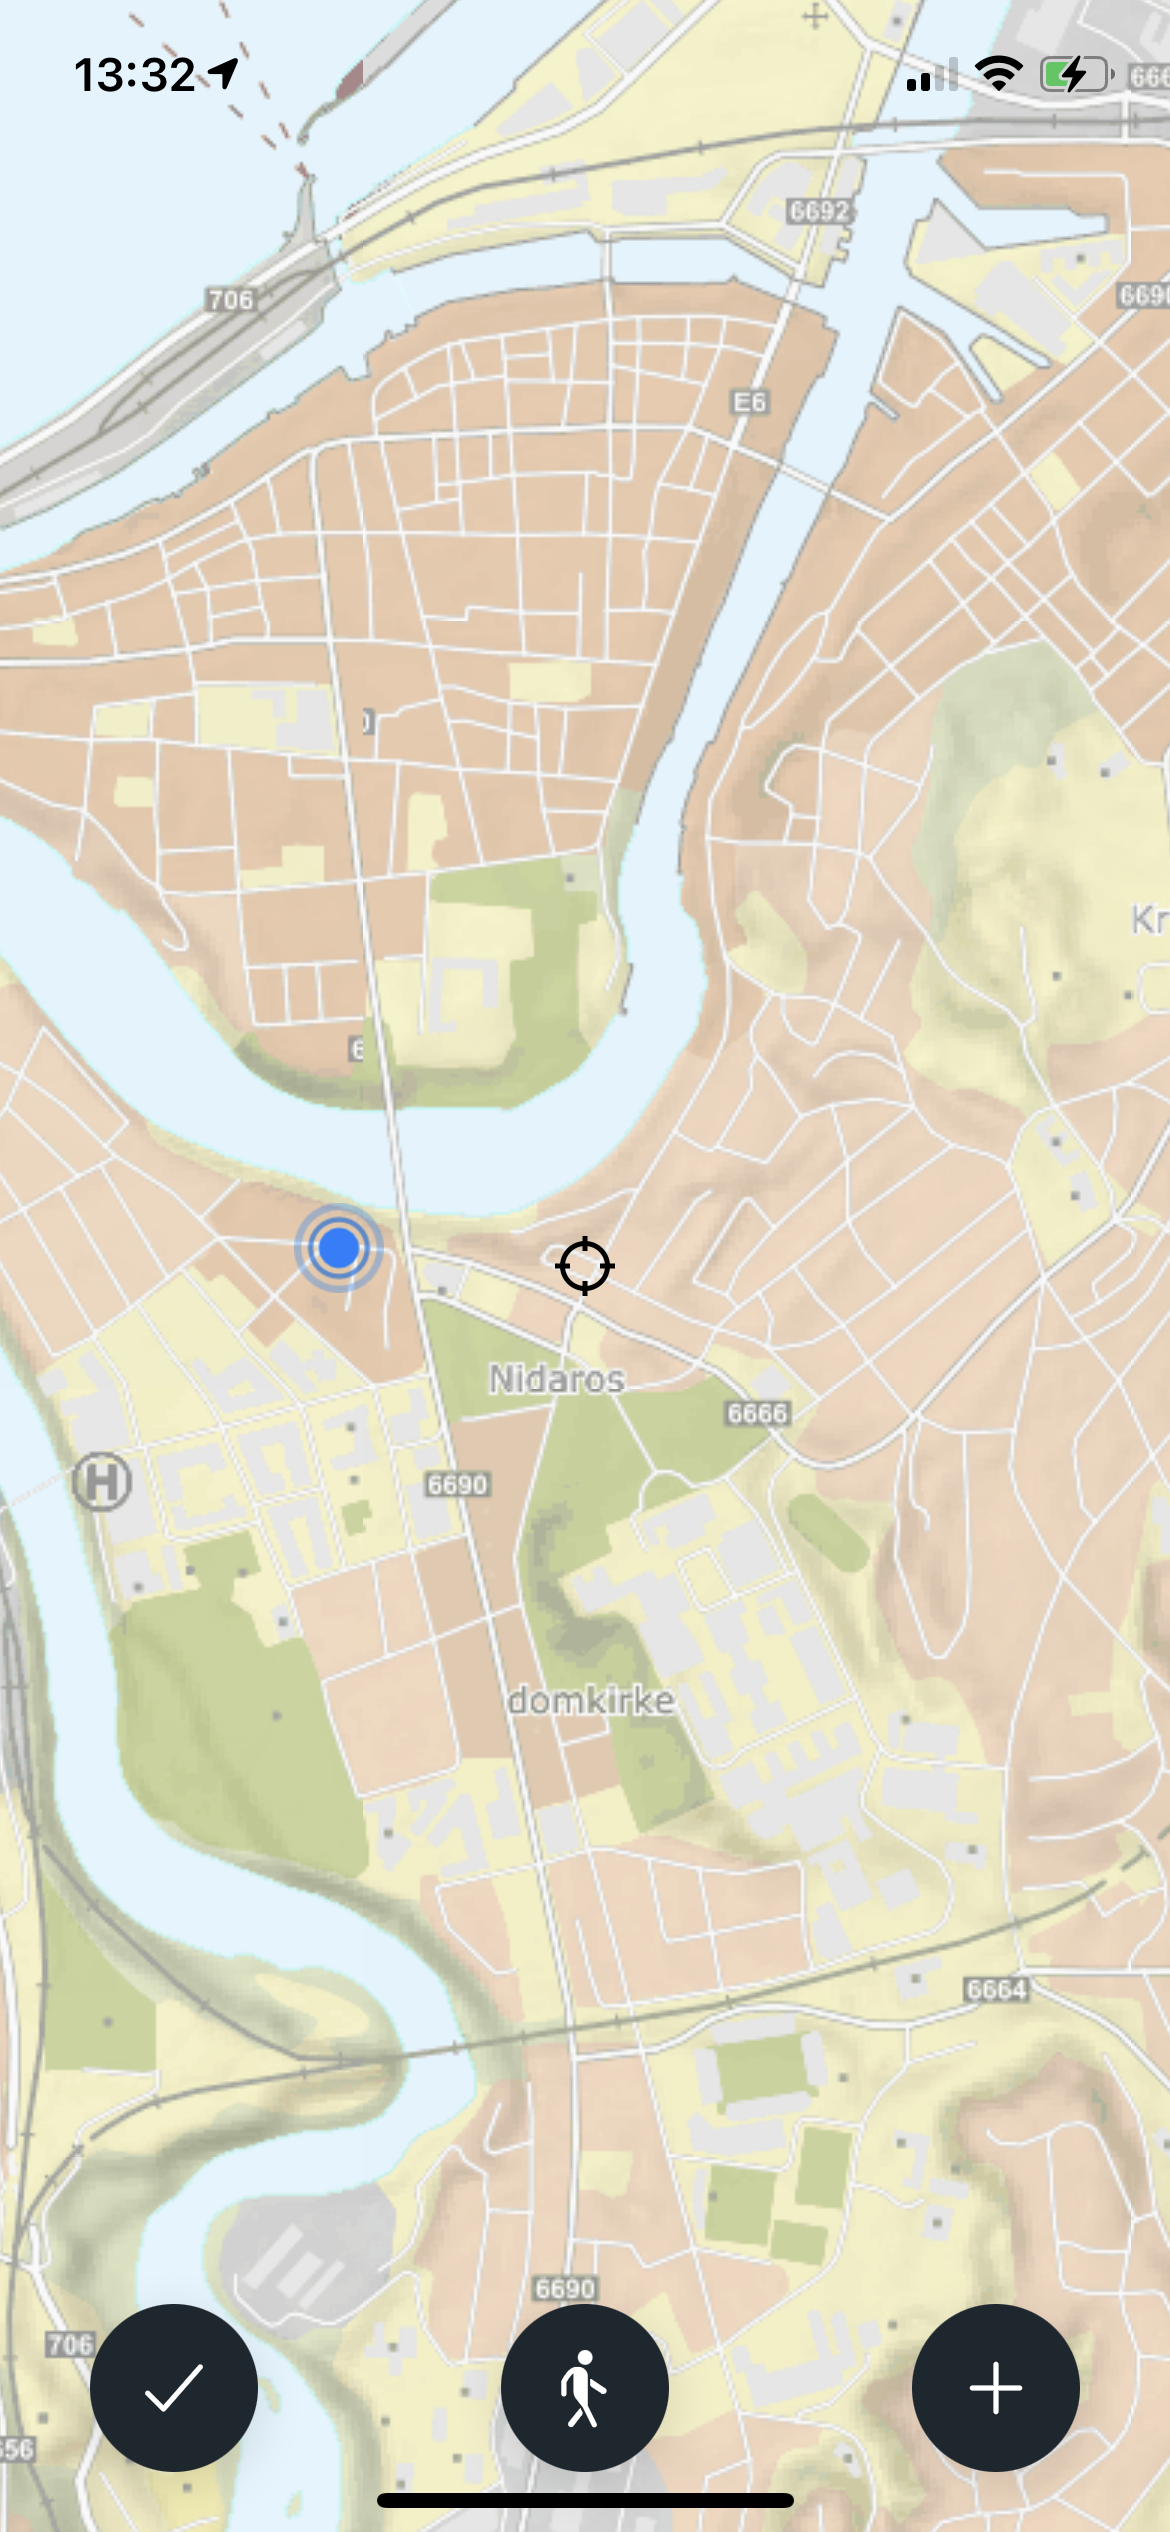
\includegraphics[scale=0.4]{Figurer/skjermbilder/kart-plain.png}
    \caption{Implementert grensesnitt for interaksjon med kart under registrering.}
    \label{fig:kart-plain}
  \end{minipage}
  \hfill
  \begin{minipage}[b]{0.4\textwidth}
    \centering
    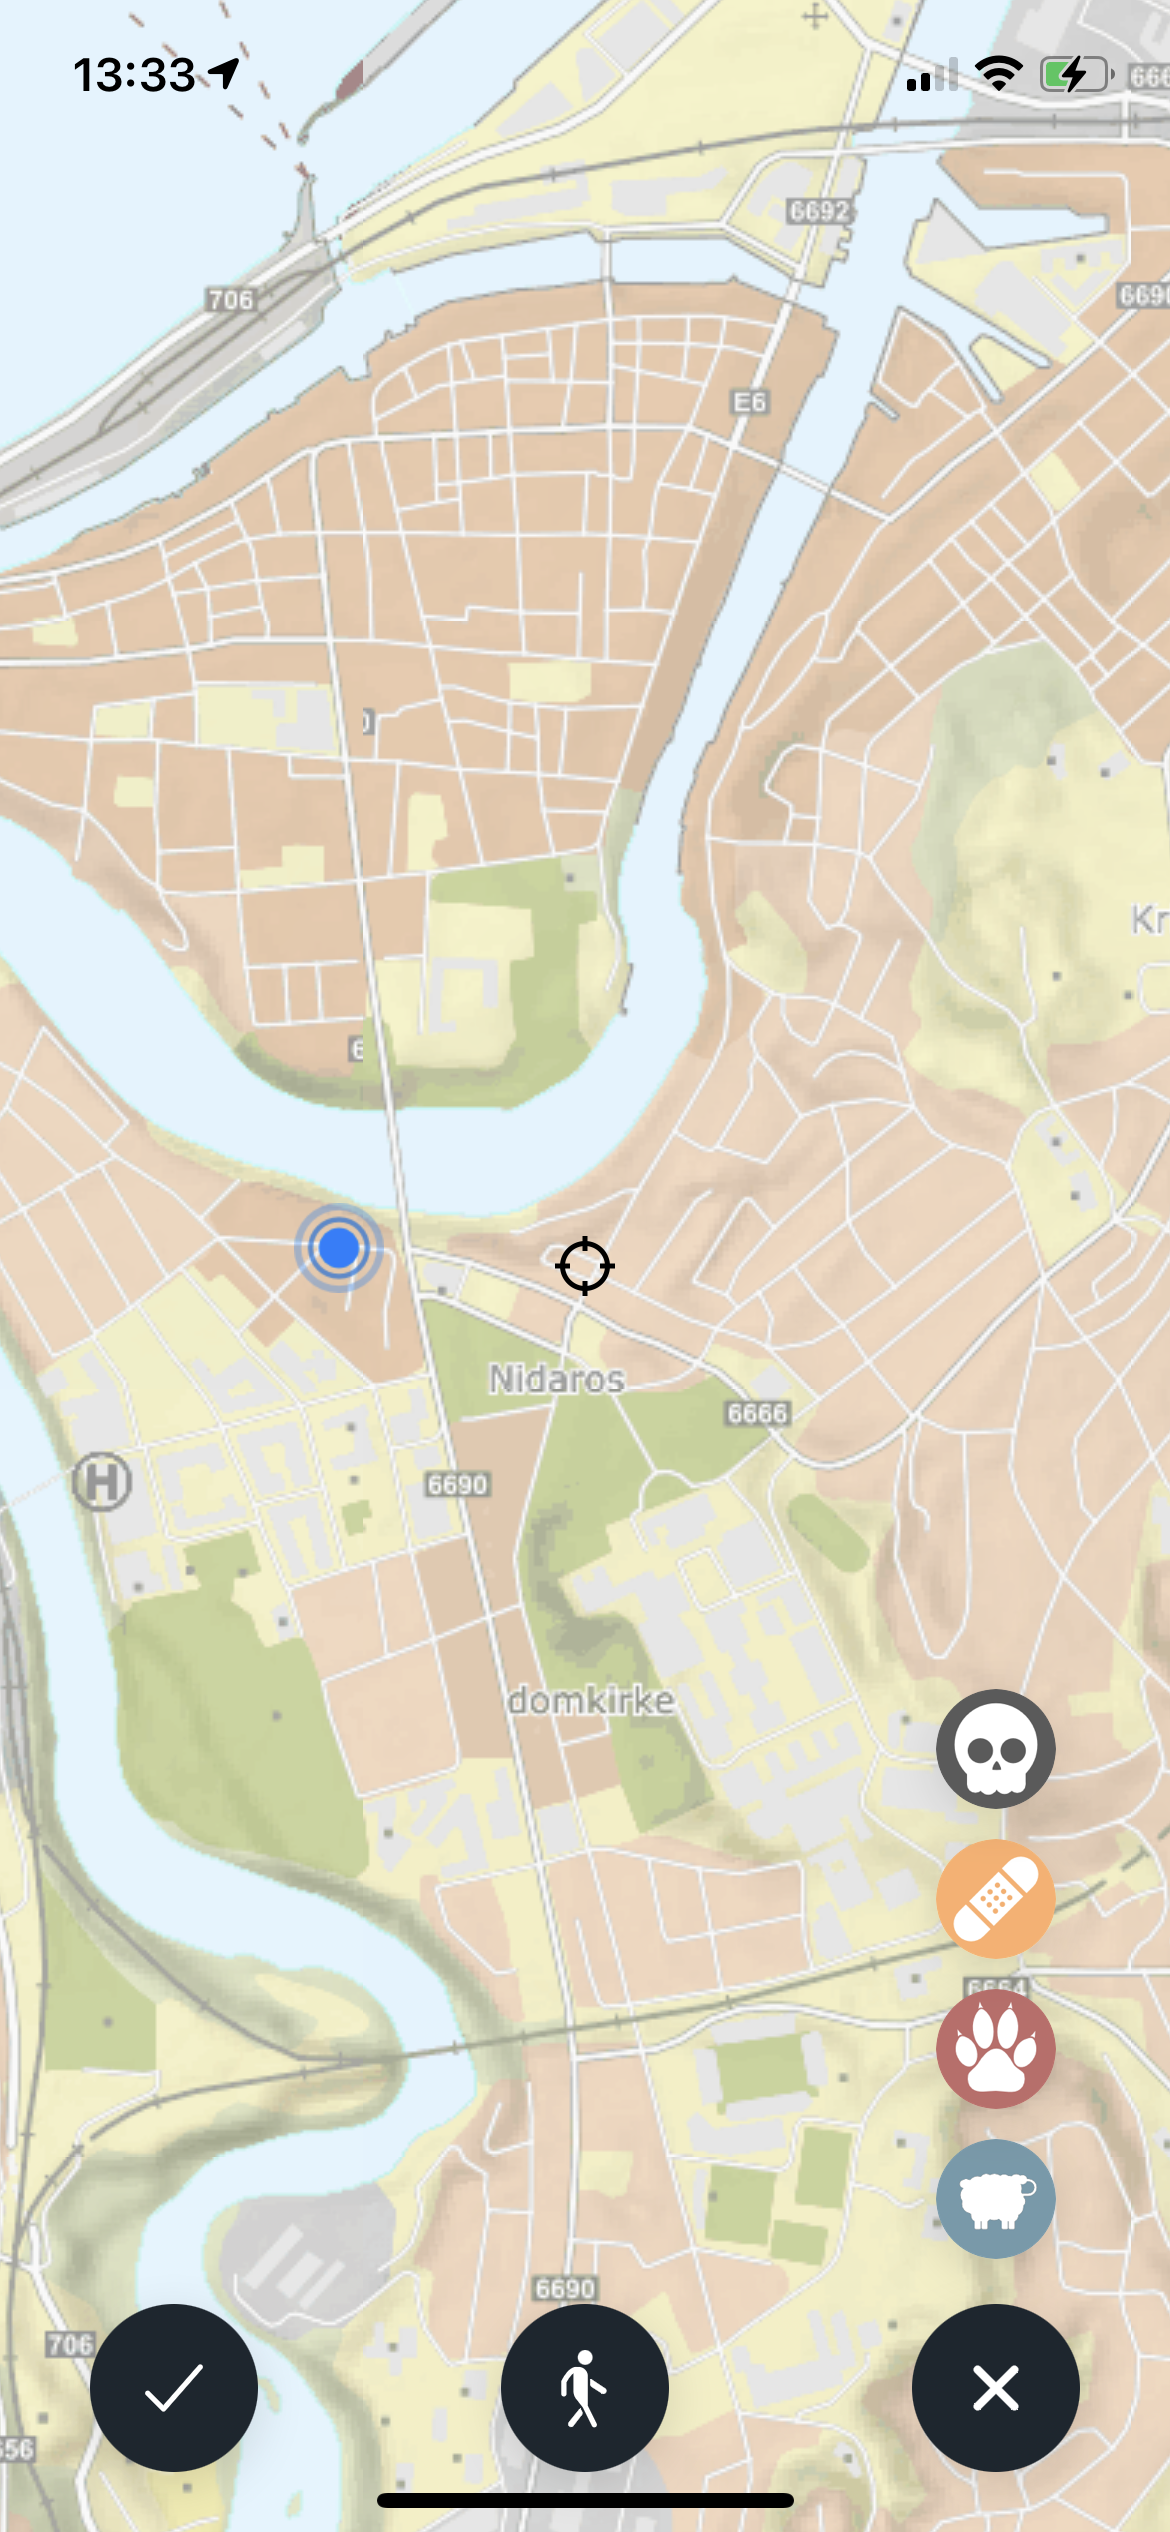
\includegraphics[scale=0.4]{Figurer/skjermbilder/kart-meny-apen.png}
    \caption{Kart-grensesnitt med åpen meny for å legge til en ny registrering.}
    \label{fig:kart-meny-apen}
  \end{minipage}
\end{figure}

\noindent
Kartgrensesnittet tar i bruk \textit{Norgeskart bakgrunn cache} \cite{NorgeskartBakgrunnCache} fra Geonorge som er utviklet av Kartverket og brukes sammen med Leaflet-biblioteket \cite{LeafletJavaScriptLibrary} for å vise fram kartet. Kartet oppdateres daglig slik at gjetere og bønder alltid vil ha tilgang til de nyeste kartbildene under en oppsynstur. Den blå markøren på kartet viser GPS-posisjonen til brukeren av applikasjonen. Markørens posisjon oppdateres i sanntid. Man kan navigere kartet ved å dra det rundt med bruk av én finger. "Pinch-zoom"-funksjonalitet er innebygd i Leaflet \cite{ZoomLevelsLeaflet} og tillater å zoome inn og ut ved hjelp av to fingre. Hvis mobiltelefonen ikke er koblet til internett vil applikasjonen automatisk velge det nedlastede kartutsnittet som passer best for den nåværende lokasjonen til mobiltelefonen. Hvis ingen nedlastede kartutsnitt passer vil brukeren få tilbakemelding om dette. Applikasjonen har også implementert funksjonalitet for å skifte mellom ulike nedlastede kartutsnitt hvis dette er nødvendig.
\newline

\noindent
For legge til en ny registrering i kartet kan brukeren trykke på pluss-knappen nede i høyre hjørne av skjermen. Dette vil åpne valg-menyen (se figur \ref{fig:kart-meny-apen}) for en ny registrering der brukeren kan velge mellom å registrere en saueflokk, et rovdyr, skadede sau eller døde sau. Menyen kan lukkes ved å trykke på den samme knappen om igjen, markert ved at pluss-tegnet har blitt byttet ut med et kryss. Registreringsmarkøren i midten av kartet plasseres over den posisjon hvor man har gjort en observasjon. Denne posisjonen brukes sammen med brukerens GPS-lokasjon, og type registrering (sau, død, skadet eller rovdyr) for å kunne legge til registreringen i kartet. Figur \ref{fig:registrert-rovdyr} viser hvordan kartgrensesnittet ser ut rett etter registrering av et rovdyr. En pin blir lagt til på kartet på posisjonen hvor observasjonen ble gjort. En striplet linje peker fra GPS-lokasjoen til brukeren under observasjonstidspunktet og fram til pinnen. Både pinnen og den striplede linjen er fargekodet for å gjøre det lettere å skille mellom ulike observasjoner.

\begin{figure}[H]
\centering
\captionsetup{width=.8\linewidth}
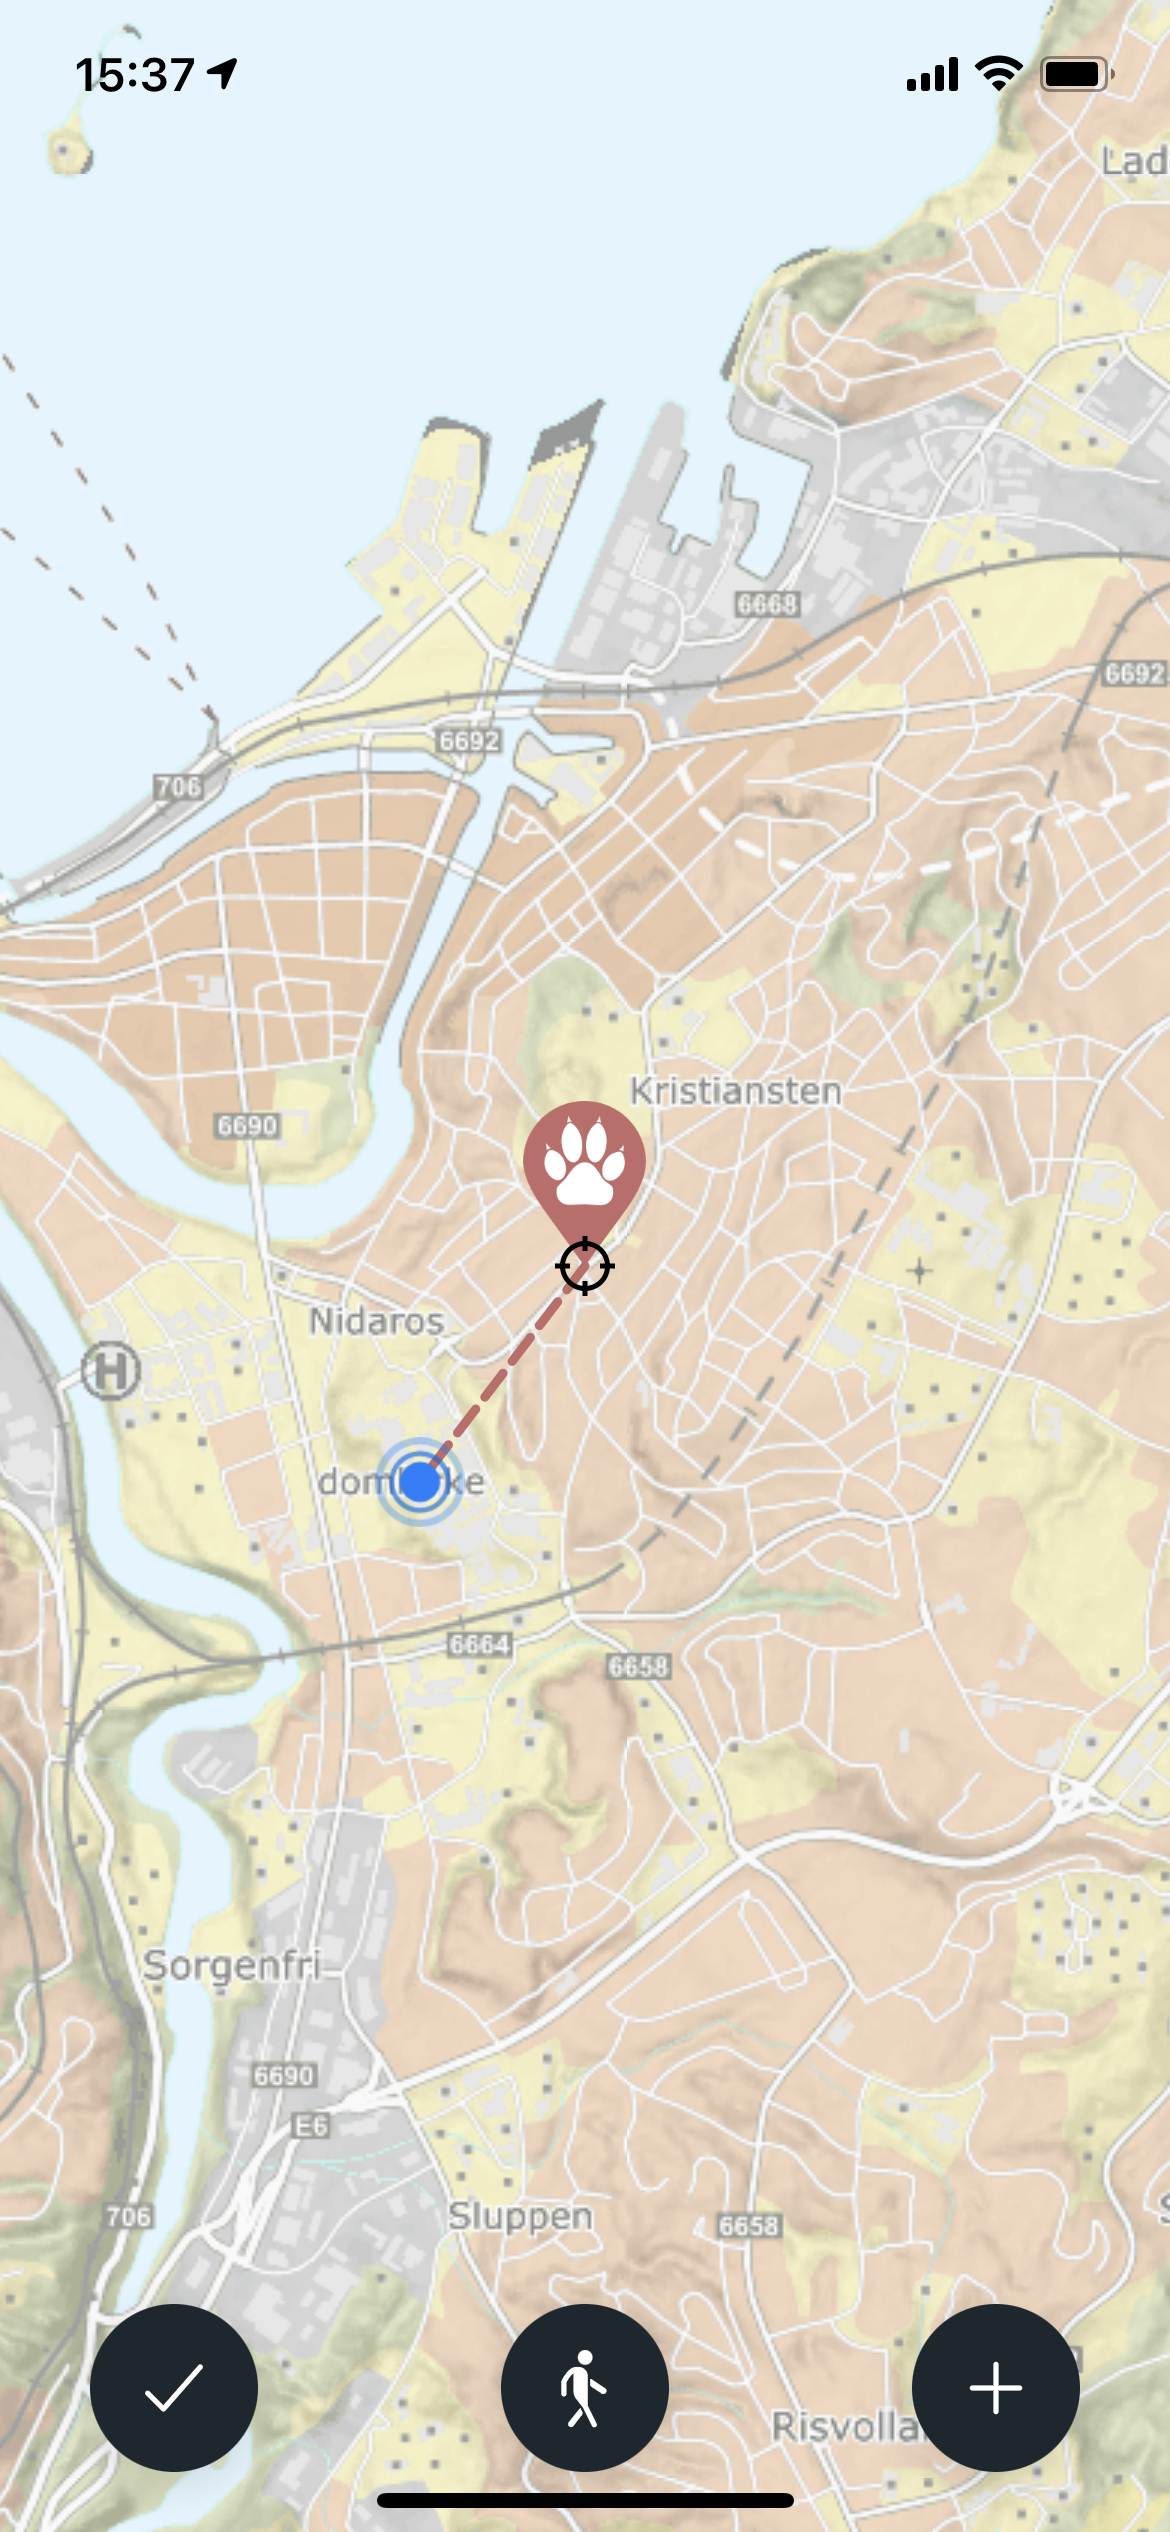
\includegraphics[scale=0.4]{Figurer/skjermbilder/registert-rovdyr.png}
\caption{Eksempel på hvordan kartgrensesnittet ser ut etter at det har blitt registrert et rovdyr.}
\label{fig:registrert-rovdyr}
\end{figure}

\subsubsection{Fullføre oppsyntur}
For å fullføre en oppsynstur trykker brukeren på fullfør-knappen nede til venstre i kartgrensesnittet (se figur \ref{fig:registrert-rovdyr}). En dialogboks, som vist i figur \ref{fig:follfore-oppsynstur}, vil da vises hvor brukeren må bekrefte handlingen. Hvis brukren trykker ja vises oppsummeringssiden fram (se figur \ref{fig:oppsynstur-oppsummering}).

\begin{figure}[H]
  \centering
  \begin{minipage}[b]{0.4\textwidth}
    \centering
    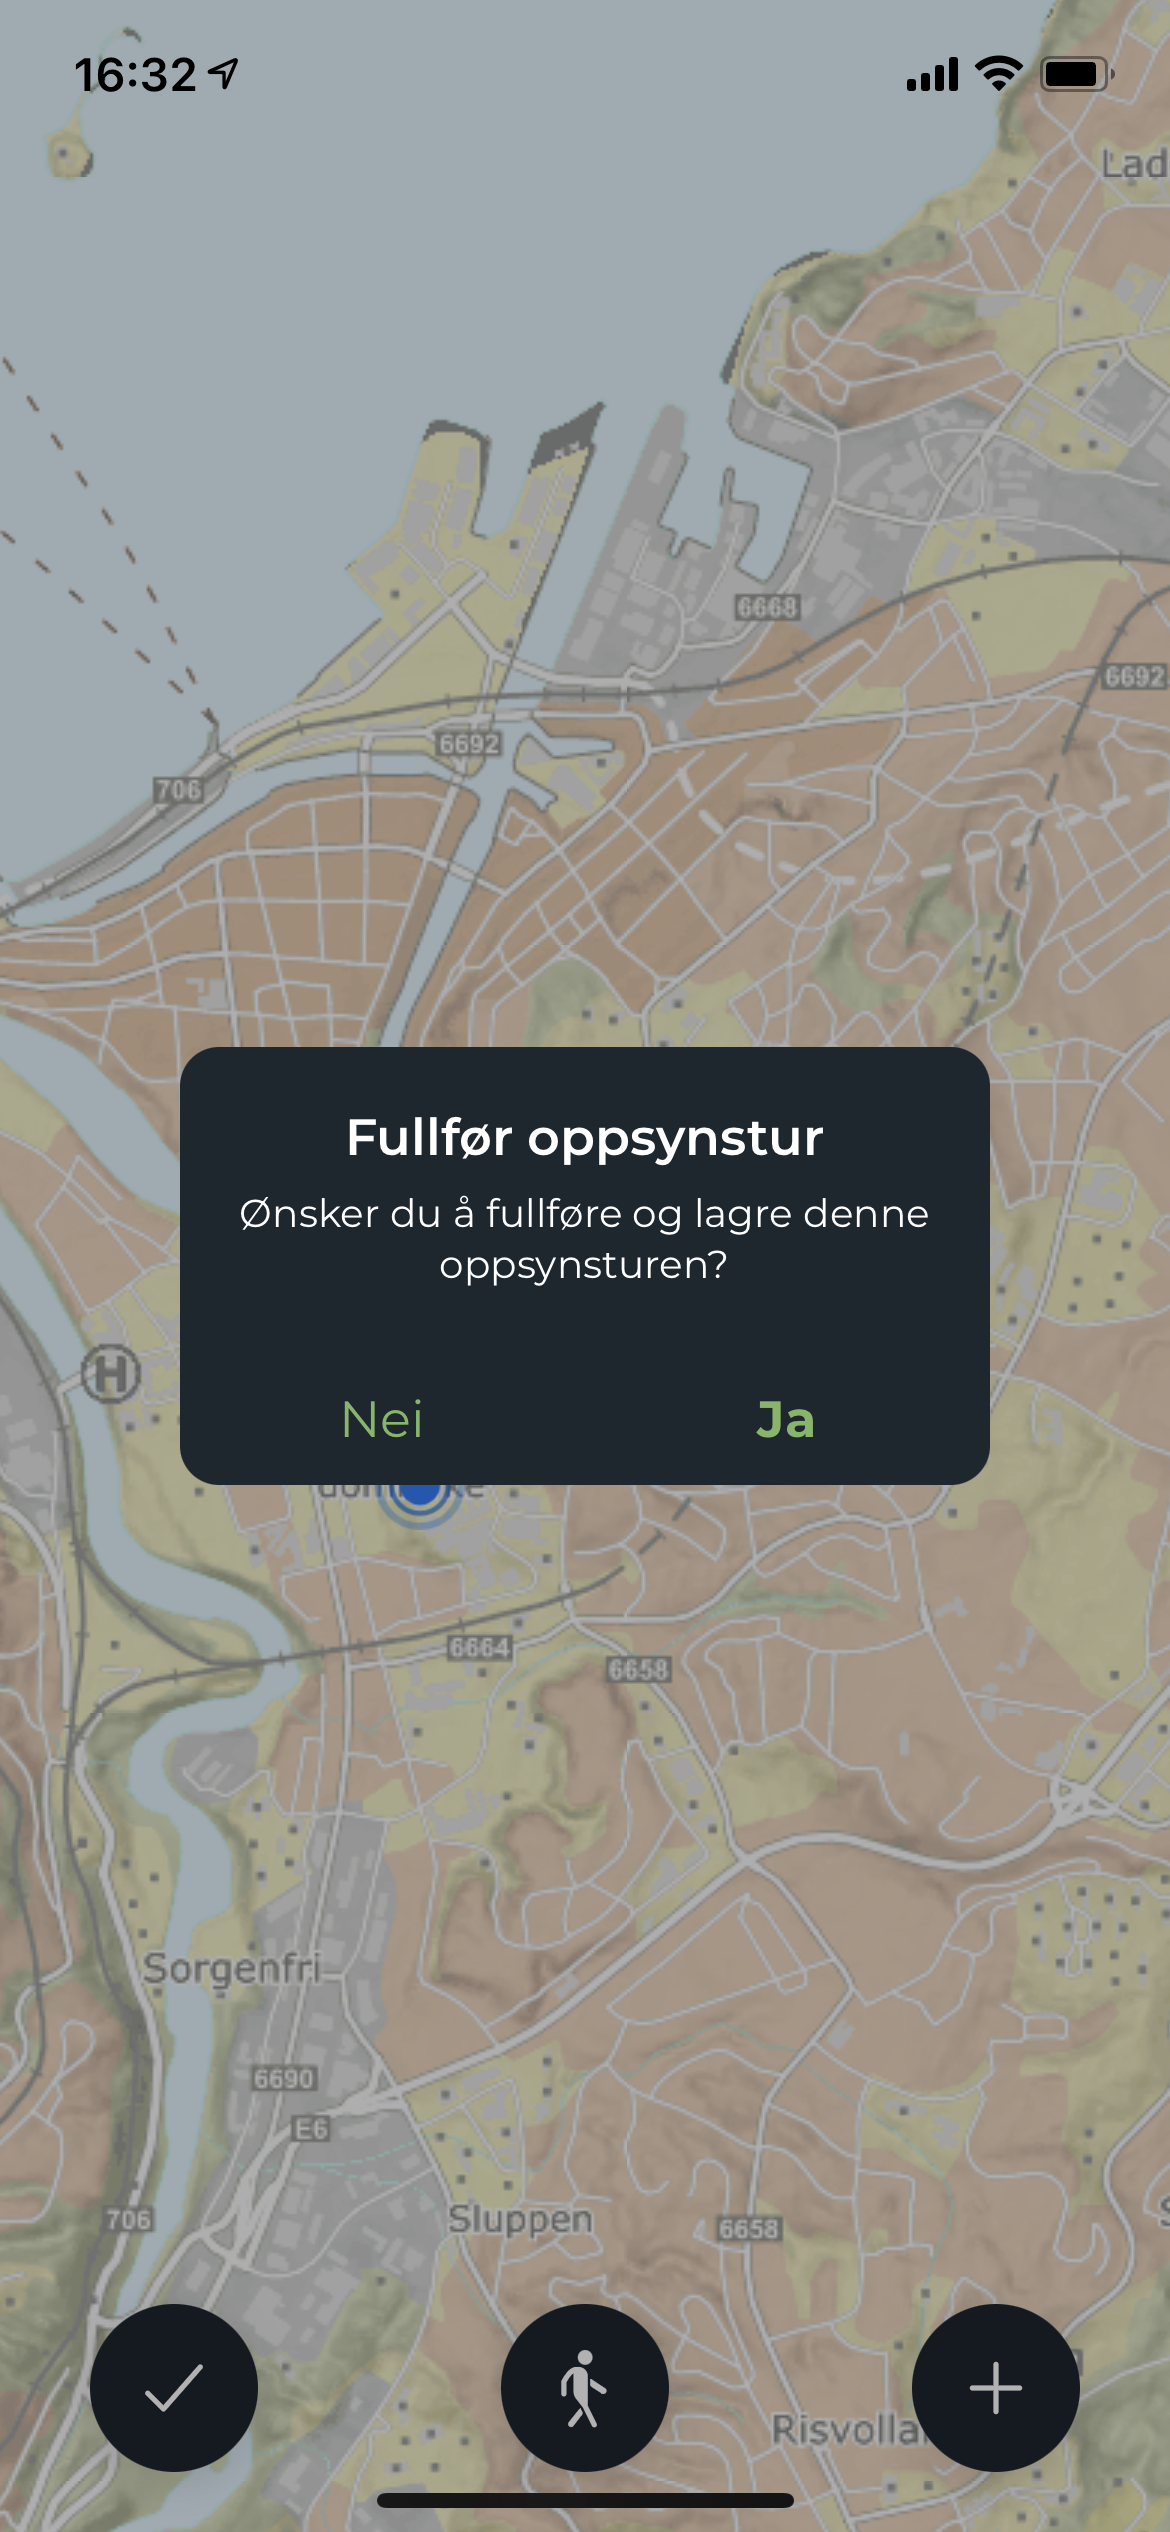
\includegraphics[scale=0.4]{Figurer/skjermbilder/follfore-oppsynstur.png}
    \caption{Dialogboks som kommer opp hvis man trykker på fullfør-knappen.}
    \label{fig:follfore-oppsynstur}
  \end{minipage}
  \hfill
  \begin{minipage}[b]{0.4\textwidth}
    \centering
    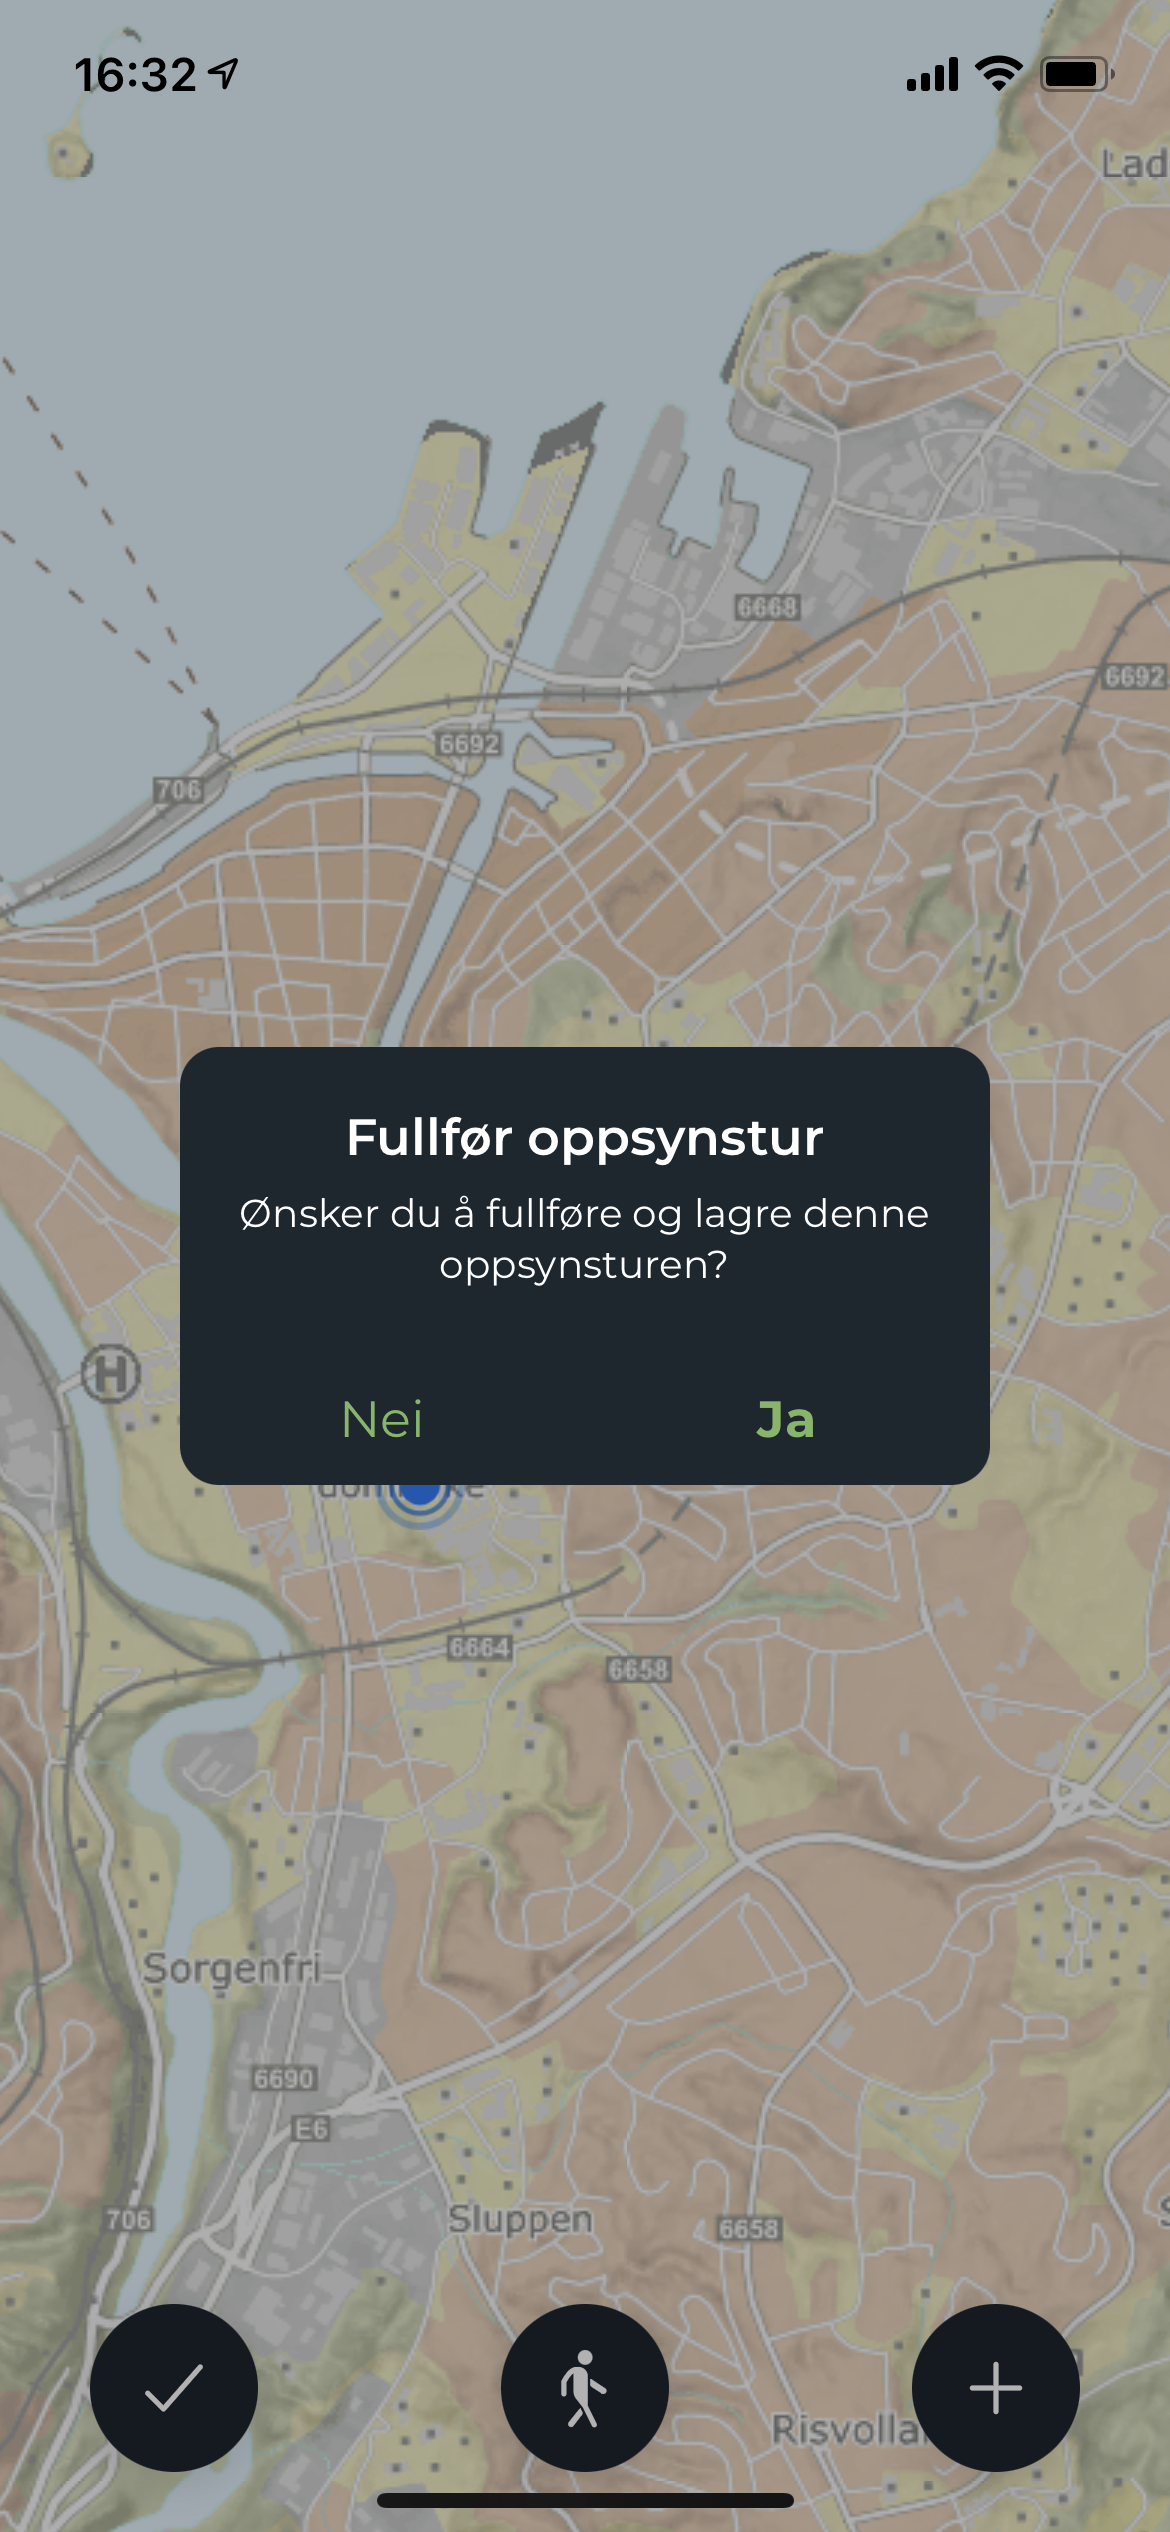
\includegraphics[scale=0.4]{Figurer/skjermbilder/follfore-oppsynstur.png}
    \caption{HER SKAL DET VÆRE ET BILDE AV EN FULLFØRT OPPSYNSTUR!.}
    \label{fig:oppsynstur-oppsummering}
  \end{minipage}
\end{figure}

\section{Bakgrunnoppdatering av GPS-lokasjon} \label{sec:bakgrunnsoppdatering-av-gps-lokasjon}
Det var opprinnelig tenkt å implementere bakgrunnsoppdatering av GPS-lokasjon under en registrering. Etter flere mislykkede forsøk på å implementere bakgrunnsoppdatering av GPS-lokasjon, endte det til slutt opp med å skrinlegge idéen og heller legge til en funksjon som ville gjøre det mulig å spare strøm mens applikasjonen kjører i forgrunnen. Ved å trykke på knappen nede i midten av kartgrensesnittet (se figur \ref{fig:registrert-rovdyr}), aktiveres gå-/strømsparings-modusen. Skjermen vil da bli svart, og en forklarende tekst som forteller hvordan man kommer seg ut av strømsparingsmodus vil vises fram før den forsvinner etter 8 sekunder. Ved å gjøre hele skjermen svart vil nyere mobilskjermer som tar i bruk OLED-teknologi kunne spare betydelig mengder strøm som ellers ville blitt brukt til å vise fram bilder på skjermen. I en undersøkelse gjort av Mian et al. \cite{dongPowersavingColorTransformation2009} utforskes bruk av mørke energisparende brukergrensesnitt for OLED-skjermer. Resultatene viser at det var mulig å bruke 75\% mindre strøm ved bruk av svarte og grønne grensesnitt framfor vanlige grensesnitt. Ettersom at applikasjonen vår viser fram en helt svart skjerm under gå-/strømsparings-modus tør vi å anta at dette tallet vil være enda høyere i vårt tilfelle.
\begin{figure}[H]
\centering
\captionsetup{width=.8\linewidth}

\includegraphics[scale=0.4]{Figurer/skjermbilder/stromsparing.png}
\caption{Skjermbilde av hvordan applikasjon ser ut rett etter at knappen for gå-/strømsparings-modus har blitt trykket på.}
\label{fig:stromsparing}
\end{figure}

\section{Tilstandshåndtering} \label{sec:tilstandshandtering}
For at applikasjonen skulle fungere som ønsket var det viktig å få på plass et solid tilstandshåndteringssystem. Med tilstandshåndtering menes det at man har programmatisk kontroll over tilstanden i applikasjonen og har mulighet til å lese eller endre denne. Hvis en del av applikasjonen endrer tilstanden, vil alle andre deler av applikasjonen få vite om dette. Tilstand kan, i vårt tilfellet, for eksempel være hvor mange søyer med grønt slips som har blitt registrert. Applikasjonen må til en hver tid å ha kontroll over hvor brukeren befinner seg i grensesnittet under registreringen av en saueflokk, samt hvilke registreringer som har blitt gjort for å kunne lese opp korrekt tekst til brukeren under en blind registrering. For å løse dette ble det bestemt å bruke NGXS. NGXS er et rammeverk og et bibliotek for tilstandshåndtering som er godt brukt og spesielt laget for Angular (NGXS omtales mer i underkapittel \ref{sub:ngxs} \nameref{sub:ngxs}). Tilstandshåndteringen for applikasjonen er delt i tre, hvor en del tar seg av hvilken kategori og underkategori brukeren er i under registrering av en saueflokk. En annen del tar seg av hvor mange sauer som har blitt registrert under hver underkategori, og den siste delen tar seg av alle registreringen som har blitt gjort for en hel oppsynstur.

\subsection{Tilstand for kategori og underkategori under registrering av saueflokk}
Tilstanden for kategori og underkategori under registrering av en saueflokk, kalt \textit{AppInfo.state} består av bare to verdier. En verdi som forteller hvilken underkategori brukeren befinner seg på (\textit{CurrentSubcategory}) og en som forteller hvilken hovedkategori brukeren befinner seg på (\textit{CurrentCategory}). \textit{AppInfo.state} inneholder også metoder for å endre og hente denne tilstanden og tilhørende informasjon.
\begin{figure}[H]
\centering
\captionsetup{width=.8\linewidth}
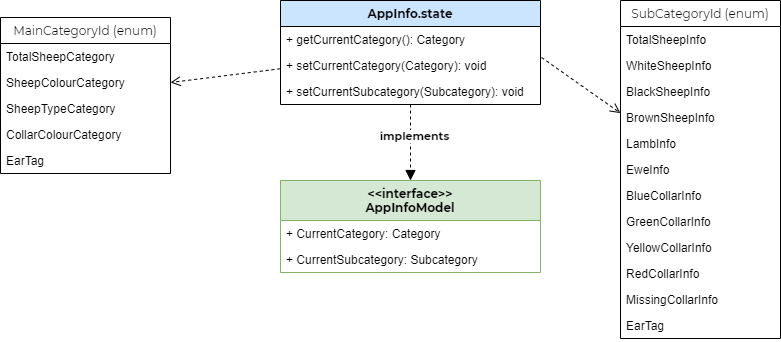
\includegraphics[scale=0.65]{Figurer/diagram/tilstand_registrering.png}
\caption{Klassediagram for tilstandshåndtering av kategori og underkategori under registrering av en saueflokk.}
\label{fig:tilstand_registrering}
\end{figure}

\subsection{Tilstand for registrering av en sauflokk}
Figur \ref{fig:tilstand_sau} viser et klassediagram for hvordan informasjonen for registreringen av en sauflokk blir delt inn i kategorier og underkategorier. Både klassen \textit{SubCategory} og \textit{MainCategory} implementerer interfacet \textit{Category}. Dette gjør det enkelt å utvide disse klassene om det skulle være nødvendig. Det samme kan man si om klassene \textit{TotalSheep}, \textit{SheepColour}, \textit{SheepType}, \textit{CollarColour} og \textit{EarTag} som alle arver fra \textit{MainCategory}. Målet med å utforme klassene på denne måten var å muliggjøre å enkelt kunne legge til enten nye kategorier eller underkategorier i framtiden.
\begin{figure}[H]
\centering
\captionsetup{width=.8\linewidth}
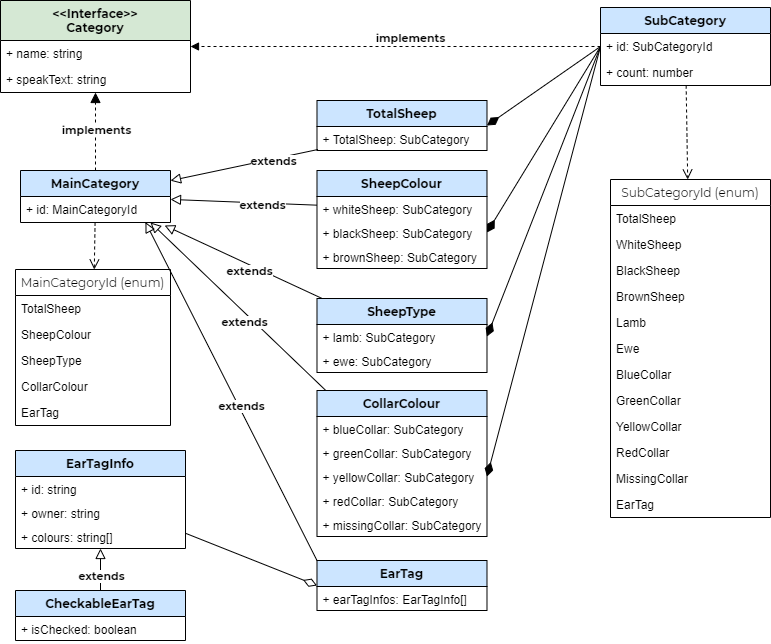
\includegraphics[scale=0.6]{Figurer/diagram/tilstand_sau.png}
\caption{Klassediagram for tilstandshåndtering av opptalte sauer del 1.}
\label{fig:tilstand_sau}
\end{figure}

\noindent
\textit{SheepInfo.state} vises i figur \ref{fig:tilstand_sau_state}. \textit{SheppInfo.state} inneholder tilstanden for all de fem hovedkategoriene, samt forskjellige metoder for å gjøre det enkelt å inkrementere eller dekrementere antallet registrerte for hver underkategori.

\begin{figure}[H]
\centering
\captionsetup{width=.8\linewidth}
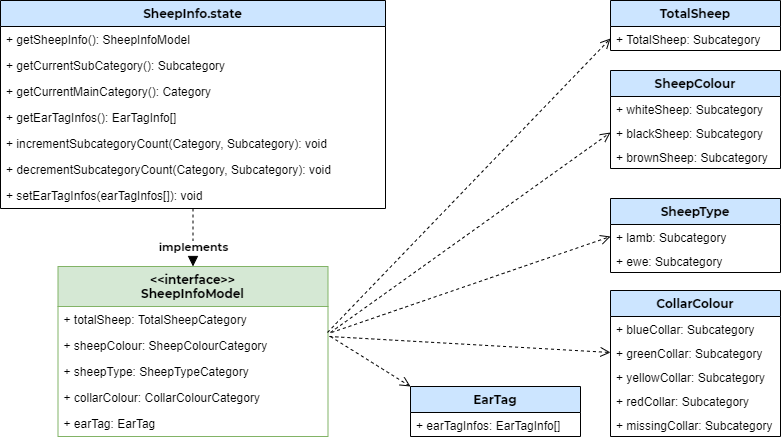
\includegraphics[scale=0.6]{Figurer/diagram/tilstand_sau_state).png}
\caption{Klassediagram for tilstandshåndtering av opptalte sauer del 2.}
\label{fig:tilstand_sau_state}
\end{figure}

\subsection{Tilstand for en oppsynstur}
I likhet med strukturen for registrering av en saueflokk er også strukturen for en oppsynstur laget modulært for å gjøre det mulig å for eksempel legge til en ny type registrering i framtiden. Klassen \textit{FieldTripInfo} innholder all informasjon som er nødvendig i forbindelse med en oppsynstur. Den inneholder også alle registreringer som er gjort i form av en liste med objekter av typen \textit{Registration}. Klassene \textit{SheepRegistration}, \textit{DeadSheepRegistration}, \textit{InjuredSheepRegistration} og \textit{PredatorRegistration} arver alle fra \textit{Registration}, noe som gjør det enkelt å legge til en ny type registrering om ønskelig. \textit{FieldTripInfo.state} inneholder én versjon av klassen \textit{FieldTripInfo}, samt metoder for å hente, oppdatere og legge til nye registreringer.
\begin{figure}[H]
\centering
\captionsetup{width=.8\linewidth}
\includegraphics[scale=0.6]{Figurer/diagram/tilstand_oppsynstur.png}
\caption{Klassediagram for tilstandshåndtering av en oppsynstur.}
\label{fig:tilstand_oppsynstur}
\end{figure}


\section{Backend}
Framfor å bruke et mer tradisjonelt oppsett med en dedikert backend-tjener og tilhørende database, bruker applikasjonen Firebase som backend i form av Backend-as-a-Service. Ettersom at Firebase har løsninger for både autentisering, autorisering og database, betydde dette at vi kunne bruke mer tid på å implementere klient-delen av applikasjonen framfor å bruke tid på eventuell backend-logikk.

\subsection{Login} \label{sub:backend-login}
For innlogging brukes Firebase Authentication gjennom Firebase Cloud. Personer som har fått tildelt en bruker kan logge seg inn ved hjelp av e-post og passord. Firebase har løsninger som tillater innlogging ved hjelp av en tredjepart som for eksempel Google eller Facebook. Dette kan enkelt implementeres på et senere tidspunkt om ønskelig. Per dags dato kan nye brukere bare registreres av utviklere gjennom konsollen til Firebase.

\subsection{Database}
For lagring av data i forbindelse med applikasjonen brukes Firebase Cloud Firestore. Cloud Firestore er en dokumentdatabase hvor dokumenter lagres i samlinger kalt \textit{collections}. Databasen er delt opp i tre forskjellige samlinger; \textit{members}, \textit{beitelag} og \textit{fieldTrips}. Samlingen \textit{members} inneholder et dokument for hver bruker av applikasjonen med informasjon om id som er knyttet til Firebase Authentication, navn, beitelagId og e-postadresse. Samlingen \textit{beitelag} inneholder et dokument for hvert beitelag som registreres i applikasjonen. Per nå kan nye beitelag bare registreres av utviklere gjennom konsollen til Firebase. Et beitelag innholder fire forskjellige data; navn, bønder (\textit{farmers}), gjetere (\textit{overseers}) og oppsynsturer (\textit{fieldTrips}). Datafeltet \textit{farmers} inneholder en liste med ider over brukere som er registrert som bønder i et beitelag. En bonde vil ha tilgang til å se på alle oppsynsturer registrert av alle brukere for et beitelag. I motsetning til dette vil brukere registrert med sin id i \textit{overseers}-listen for et beitelag bare ha tilgang til å se oppsynsturer registrert av seg selv. Logikken for dette ligger i Firestore Security Rules og håndteres på tjenersiden av Firebase. Hvert beitelagsdokument peker til en egen \textit{fieldTrips}-samling som inneholder alle oppsynsturene som er registrert for det gitte beitelaget.

\begin{figure}[H] 
\centering
\captionsetup{width=.8\linewidth}
\includegraphics[scale=0.6]{Figurer/diagram/databasestruktur.png}
\caption{Databasestrukturen for Cloud Firestore.}
\label{fig:databasestruktur}
\end{figure}

\noindent
Figur \ref{fig:firebase_baas} viser en flyt for innlogging og registrering av en oppsynstur ved hjelp av Firebase. Når en bruker åpner applikasjonen på mobilen sin (klient) vil brukeren bli bedt om å oppgi brukernavn og passord. Dette sendes til Firebase Authentication som sjekker om opplysningene er korrekte og deretter gir brukeren tilgang til applikasjonen. Når brukeren skal laste opp en oppsynstur går kallet gjennom Firestore Security Rules. Her sjekkes det som brukeren er logget inn, om oppsynsturen inneholder alle nødvendige data og om brukeren er den den oppgir seg for å være og er registrert i det oppgitte beitelaget. Om alt er som det skal lagres oppsynsturen i Cloud Firestore som et dokument i \textit{beitelag}-samlingen. En bekreftelse sendes deretter tilbake til brukeren og forteller om alt gikk som den skulle.

\begin{figure}[H] 
\centering
\captionsetup{width=.8\linewidth}
\includegraphics[scale=0.8]{Figurer/diagram/firebase_baas.png}
\caption{Diagrammet viser interaksjon mellom BaaS og en klient for innlogging og lagring av en ny oppsynstur.}
\label{fig:firebase_baas}
\end{figure}


\section{Konklusjon}

\noindent
Løsningen som har blitt implementert for å muliggjøre bruk av offline-kart møter kravet F1 spesifisert i kravspesifikasjonen (se tabell \ref{tbl:funksjonelle-krav}). F1 sier at kartet skal ta i bruk Kartverkets tjenester i form av NorgesKart. Dette kravet innfris ved bruk av cache-tjenesten til Geonorge, som er utviklet av Kartverket. Krav F1 spesifiserer også at brukeren skal ha tilgang til de mest oppdaterte kartbildene. Dette løses ved at det er mulig å oppdatere et kartutsnitt enkelt gjennom grensesnittet som vist ved \enquote{Oppdater}-knappen i figur \ref{fig:nedlastede-kartutsnitt-apen-meny}. Løsningen tilfredsstiller også det funksjonelle kravet F1.1 (se tabell \ref{tbl:funksjonelle-krav}), som sier at brukeren skal kunne laste ned et kartutsnitt som skal kunne benyttes når mobilen ikke har tilgang på internett. Det har blitt implementert funksjonalitet for å vise fram brukerens rute, samt mulighet for å registrere observasjoner i form av pins på kartet. Dette oppfyller de funksjonelle kravene F1.2 og F1.3. Alle krav og underkrav for F2 har blitt innfridd. All nødvendig informasjon som farge på sau, slips, øremerker og om de er søye eller lam kan registreres om brukeren ønsker det. Nye øremerker kan legges til med navn på tilhørende bonde og inntil to forskjellige farger. Når en oppsynstur avsluttes gis det tilbakemeldinger på om det har oppstått avvik i registreringen av en saueflokk. Registreringer lagres også eksternt i Firebase Cloud Firestore, noe som gjør det mulig å dele oppsynsturer med alle i samme beitelag. Kravet F3, \textit{Systemet skal ha innlogging med brukernavn og passord} har blitt nådd ved hjelp av Firebase Authentication. Kravet F1.3, \textit{Brukeren skal ha egen profil og mulighet til å se og endre på den}, har ikke blitt implementert da dette ikke ble sett på som viktig nok funksjonalitet. Alle krav og underkrav for F4 ble innfridd allerede under fordypningsprosjektet.
\newline
\newline
\noindent
 De ikke-funksjonelle kravene har IF1, \textit{Applikasjonen skal fungere uten internett} og IF2, \textit{Applikasjonen skal være kryssplattform ...} har blitt oppnådd. Kravet IF3 har ikke blitt testet i denne omgang. Kravet IF4 ble testet i fordypningsprosjektet, hvor det kom fram at en kombinasjon av haptisk tilbakemelding, tekstopplesing, samt interaksjon gjennom sveiping og trykking på grensesnittet for blind registrering var det mest effektive.
\part{Resultater}

\chapter{Brukertest}
I dette kapittelet skal teorien bak brukervennlighetstester kort presenteres og valget av brukervennlighetstest begrunnes. Deretter skal forberedelsene og gjennomføringen av brukertestene beskrives i detalj. 

\section{Brukervennlighetstester}
Det finnes ingen offisiell definisjon på hva som kjennetegner en brukervennlighetstest. Ekspert på brukeropplevelse (\acrshort{ux}) Steve Krug definerer brukervennlighetstester som \cite[~s.13]{krugRocketSurgeryMade2010}: 
\begin{displayquote}
\textit{Å observere folk som prøver å bruke det du designer/utvikler/bygger (eller noe som du allerede har designet/utviklet/bygget) med intensjonen om å gjøre det enklere for folk å bruke eller bevise at det er enkelt i bruk}.
\end{displayquote}
Det er vanlig å kategorisere brukervennlighetstester i to ulike kategorier: kvalitative og kvantitative brukertester. 
\newline
\newline
Kvalitative brukertester går ut på å innhente funn fra observasjoner som kan identifisere designfunksjoner som er enkle eller vanskelige å bruke \cite{budiuQuantitativeVsQualitative2017}. Det betyr med andre ord at målet med slike brukervennlighetstester er å få innsikt som gjør at produktet som utvikles kan forbedres \cite[~s.14]{krugRocketSurgeryMade2010}. Ettersom målet ikke er å samle inn sammenlignbar data for å kunne bevise noe, er kvalitative brukertester gjerne mer uformelle i strukturen og protokollene kan gjerne endres på under gjennomføringen hvis det ses på som nødvendig \cite[~s.14]{krugRocketSurgeryMade2010}. Slike tester gjennomføres ofte med få brukertestdeltakere der de får oppgaver som skal løses mens de forteller hva de tenker når de samhandler med applikasjonen i en såkalt tenk-høyt protokoll, slik at observatørene kan notere hva deltakerene tenker om applikasjonen \cite{HvaErThink}. 
\newline
\newline
Kvantitative brukertester går ut på å innhente målbar data for å vurdere om oppgavene var enkle eller vanskelige å utføre \cite{budiuQuantitativeVsQualitative2017}. Det vil si at målet med kvantitative brukertester er å bevise noe ved å samle inn data som kan måles, slik som suksessrate, tid eller antall feil for å kunne trekke en konklusjon \cite[~s.13]{krugRocketSurgeryMade2010} \cite{budiuQuantitativeVsQualitative2017}. Derfor har slike brukertester en mye mer gjennomtenkt og strukturert testprotokoll som skal følges konsekvent for alle deltakere. Dette gir også et større behov for mange testdeltakere for å kunne trekke statistiske konklusjoner \cite[~s.13]{krugRocketSurgeryMade2010} .
\newline
\newline
I fordypningsprosjektet ble brukertester utført for å konkludere hvilket brukertest var best egnet for registrering av sau i blinde ved å samle data på hvor lang tid deltakerne brukte på å registrere, feilrate og tilbakemeldinger fra deltakerene hentet fra en spørreundersøkelse med spørsmål fra \acrfull{sus}. Disse testene var dermed i hovedsak kvantitative brukertester med elementer fra kvalitative brukertester ettersom spørreundersøkelsen gitt til deltakerne ble utformet for å hente kvalitative tilbakemeldinger for å forbedre funksjonaliteten i applikasjonen til den videre utviklingen under masteroppgaven. Under brukertestene for masteroppgaven skal deltakerne teste hele systemet for å finne ut hva som kan forbedres i applikasjonen. Disse testene er derfor kvalitative brukervennlighetstester. 

\section{Gjennomføring av brukertest}
Selv om kvalitative brukertester er mindre strukturerte og mer uformelle enn kvantitative brukertester, ble det utformet en plan for hvordan brukertestene skulle gjennomføres. Dette var for å forsikre at alle funksjonene som det var ønskelig å få tilbakemelding på skulle utføres av deltakerne og at samme rute ble fulgt ettersom applikasjonens GPS-funksjonalitet også skulle utprøves i testene. Det ble i tillegg bestemt at det ikke var nødvendig å teste grensesnittet for registrering i blinde ettersom det allerede var gjennomført og vurdert i fordypningsprosjektet.

\subsection{Valg av testdeltakere}
Med kvalitative brukertester er det ikke behov for mange testdeltakere ettersom det fleste store feil vil bli oppdaget tidlig og videre testing på flere deltakere vil ikke gi mer innsikt \cite[~s.43]{krugRocketSurgeryMade2010} \cite{budiuQuantitativeVsQualitative2017, renwickHowManyParticipants2019}. Det vanligste antallet testedeltakere for kvalitative tester er 5 \cite[~s.43]{krugRocketSurgeryMade2010} \cite{budiuQuantitativeVsQualitative2017, renwickHowManyParticipants2019}, og dette ble brukt som utgangspunkt for brukertestene for masteroppgaven. Opprinnelig var det ønsket å utføre brukertestene på minst én saubonde for å undersøke om applikasjonen innfridde deres behov under oppsynsturer, men på grunn av den pågående koronaviruspandemien ble dette vanskelig (les mer i underkapittelet \enquote{\nameref{korona}}). Dermed måtte brukertesten testes på utviklerenes eksisterende nærkontakter. Enkelte av disse hadde vært med i gjennomføringen av brukertestene for fordypningsoppgaven som gikk ut på å teste grensesnittet for registrering. I disse brukertestene fikk testdeltakerne en demonstrasjon og innføring i hvordan registreringen fungerte i applikasjonen, og disse deltakerne var dermed godt kjent med dette grensesnittet. Dette ble sett på som en mulighet til å undersøke om det var en forskjell mellom brukerne som tidligere var kjent med grensesnittet for registrering og brukere som ikke fikk demonstrasjon i det hele tatt. Det ble derfor valgt ut 2 deltakere som ikke hadde kjennskap til applikasjonen og 3 deltakere som hadde vært med på tidligere brukertester og var kjent med deler av brukergrensesnittet. Ellers ble ingenting annet lagret om testdeltakernes demografi, som kjønn eller alder av hensyn til personvern.

\subsection{Før testen}
En av utviklerene vil få rollen som forsøksleder og den andre som observatør, og dette avgjøres før testen. Forsøkslederens ansvar er å informere deltakere om hvordan testen skal foregå og følge planen som er utarbeidet for gjennomføringen av brukertesten slik at det blir utfort på riktig måte. Observatøren skal under hele testens forløp observere deltakerne og notere deres kommentarer på en strukturert og oversiktlig måte. For å forsikre at ble startet på like premisser, ble det utformet en sjekkliste som skulle utføres på før selve brukertesten: 
\begin{enumerate}
    \item Fjerne tidligere oppsynsturer som er blitt gjennomført på testbrukeren. 
    \item Fjerne tidligere kartutsnitt.
    \item Skru av skjermsparer
    \item Desinfisere mobiltelefonen (mer om smittevernstiltak er utdypet i kapt. \ref{korona}).
\end{enumerate}
\noindent
For å være sikker på at alle testdeltakerne fikk lik informasjon om hvordan testen skal foregå, ble det også utformet et skriv som forsøksleder leser opp fra før testen gjennomføres: 
\begin{enumerate}
    \item Forsøksleder introduserer seg selv og observatøren.
    \item Forsøksleder forklarer hensikten med brukerstesten: 
    \newline
    \textit{"Jeg vil at du skal se for deg at du er en sauebonde, og du skal sjekke hvordan det står til med saueflokken din som er på utmarksbeite for sommeren. Det er viktig at du raskt oppdager om det er skadet, død eller rovdyr på beitet slik at du kan griper inn med tiltak.
    På oppsynsturer skal du sjekke hvor mange sauer det er totalt, hvor mange sauer det er av hver farge, antall søyer og lam og antall sauer som har slips (som er en krage rundt halsen med farge som viser hvor mange lam en søye skal ha) og sauenes øremerker. Problemet er at disse sauene ofte går langt og beveger seg hele tiden, så det er en utfordring å få øye på dem. Derfor foregår registrering av sau som oftest mens man observerer sauene gjennom kikkert. I tillegg vil observasjoner av skadet, død sau eller rovdyr bli registrert dersom det oppdages på turen. I denne brukertesten skal du teste en applikasjon som skal bistå som verktøy for å registrere oppsynsturer for sau."}
    \newline
    \newline
    \textbf{Husk at det er systemet vi evaluerer og tester, ikke deg. Vi skal ikke teste hvor flink du er til å bruke appen, men hvor bra appen fungerer for deg.}
    \item Forsøksleder forklarer hvordan brukertesten gjennomføres:
    \newline
    \textit{"Vi har laget en rute for en oppsynstur der vi vil gi deg oppgaver som du skal løse med appen underveis. Det vil være 8 oppgaver til sammen.  Du kan bryte brukertesten når som helst. Si gjerne hva du tenker mens du løser oppgavene. Hvis du sliter og sitter fast med en oppgave, kan du spørre om hjelp fra forsøksleder, ellers vil ikke forsøksleder eller observatør kommentere underveis."}
    \item Deltakeren får mulighet til å spørre spørsmål og om noe er uklart.
\end{enumerate}

\subsection{Selve brukertesten} \label{brukertest}
Brukertestene ble gjennomført ved at forsøksleder, testdeltakeren og observatøren gikk en planlagt rute ved campus Gløshaugen i Trondheim, se figur  under. Forsøksleder ga testdeltakeren oppgaver underveis, og det var tilsammen 8 oppgaver med tilhørende deloppgaver som skulle utføres under turen:

\begin{figure}[H]
\centering
\captionsetup{width=.8\linewidth}
\includegraphics[scale=0.5]{Figurer/Bilder/brukertest_rute_med_pins.png}
\caption{Rute for brukertestene på Gløshaugen campus}
\label{fig:brukertest_rute}
\end{figure}
 
\renewcommand{\labelenumii}{\theenumii}
\renewcommand{\theenumii}{\theenumi.\arabic{enumii}.}
\begin{enumerate}[font=\bfseries]
    \item \textbf{Last ned kartutsnitt}
    \begin{enumerate}
        \item Endre navnet på det nedlastede kartutsnittet. 
    \end{enumerate}
    \item \textbf{Ny oppsynstur}
    \begin{enumerate}
        \item Legg til alle deltakere som er med på turen (testdeltaker, forsøksleder og observatør).
        \item Skriv inn beskrivelse om ønskelig.
    \end{enumerate}
    \item \textbf{Registrere sauer}
    \begin{itemize}
        \item Gå til Kolbjørn Hejes vei 8. Registrer sauer ved toget på andre siden av plenen.
        \begin{enumerate}
            \item 5 sauer totalt.
            \item 3 hvite, 1 svart og 1 brun.
            \item 2 søyer og 3 lam.
            \item 1 grønt og 1 gul slips.
            \item Registrer nytt øremerke med navn og farge og velg dette øremerket.
            \item Fullfør registreringen.
        \end{enumerate}
    \end{itemize}
    \item \textbf{Registrer rovdyr}
    \begin{itemize}
        \item Gå til 7034 Trondheim. Registrer rovdyr på fotballbanen.
        \begin{enumerate}
            \item Registrer observasjon av gaupe.
            \item Skriv kommentar om ønskelig.
        \end{enumerate}   
    \end{itemize}
    \item \textbf{Registrer død sau}
    \begin{itemize}
        \item Gå til trappene ved hovedbygningen. Registrer død sau ved krysset nedenfor. 
        \begin{enumerate}
            \item 1 dødt dyr.
            \item Skriv kommentar om ønskelig.
            \item Ta et bilde.
            \item Fjern bildet.
            \item Fullfør registrering.
        \end{enumerate}
    \end{itemize}
    \item \textbf{Registrer skadet sau}
    \begin{itemize}
        \item Gå til 7030 Trondheim. Registrer skadede sauer på broa rett fram.  
        \begin{enumerate}
            \item Registrer 2 skadede sau.
            \item Skriv kommentar om ønskelig.
        \end{enumerate}
    \end{itemize}
    \item \textbf{Fullfør oppsynstur}
    \begin{enumerate}
        \item Sjekk om registreringene stemmer.
        \item Oppdater beskrivelse om ønskelig.
        \item Trykk "Fullfør". 
    \end{enumerate}
\end{enumerate}

\subsection{Etter testen}
Etter testen ble testdeltakerne spurt om de hadde noen generelle tilbakemeldinger og deres helhetlige inntrykk av applikasjonen. 

\subsubsection{Gjennomføring av brukertest under Covid-19} \label{korona}
Gjennomføringen av brukertestene har vært sterkt preget av den pågående Covid-19 pandemien for både fordypningsprosjektet og masteroppgaven. Selv om det var svært lite smitte i Trondheim da brukertestene skulle gjennomføres, ble det innført strenge nasjonale smittevernstiltak 23.03.21, dagen før det var planlagt å utføre brukertestene. Økt avstand og færre nære kontakter er to sentrale smittereduserende tiltak i håndteringen av koronapandemien ifølge \acrfull{fhi} \cite{AvstandOgFaerre2020}. Derfor ble det tatt noen forholdssregler og iverksatt smittevernstiltak under selve brukertestene slik at brukertestene ble gjennomført på en trygg måte og tilfredstilte \acrshort{fhi} sine råd og anbefalinger. Det ble bestemt at alle testdeltakerne skulle være venner som allerede ble betegnet som utviklerens nærkontakter slik at ingen utenforstående eller utviklerne selv måtte bli utsatt for særskilt risiko. Dette medførte at alle testdeltakerne var medstudenter i 20-årene. For å få best mulig data ville det vært mer optimalt med en jevnere demografisk spredning av deltakerne og testing av faktiske sauebønder, men det ble uaktuelt i en slik smittesituasjon. I tilegg ble det også utført praktiske smittevernstiltak for å sørge for at brukertestene ble tryggest mulig. Mobiltelefonen som testdeltakerne benyttet seg av i brukertestene ble desinfisert før og etter testen og utviklerne sørget for å holde minst 2 meter avstand slik de daværende smittereglene anbefalte. 

\section{Konklusjon}
Det ble utført brukervennlighetstester på Sauron for å få tilbakemeldinger på hvor godt egnet applikasjonen er til å bistå i registrering av sau på oppsynstur. Testene som ble gjennomført var såkalte kvalitative tester med fokus på å avdekke problemområder i designen og funksjonaliteten til applikasjonen. Det ble utformet en plan og rute for gjennomføringen av brukertestene som ble fulgt. Tilsammen 5? personer ble testet. På grunn av den pågående Covid-19 ble det satt smittevernstiltak og begrensninger for brukertestene, særlig for demografien til testdeltakerne. 
\chapter{Resultater fra brukertestene} \label{resultater}
Dette kapittelet skal presentere resultatene fra de fem brukervennlighetstestene som ble gjennomført. Det vil innebære kvalitative resultater som observasjoner av testdeltakerene mens de utfører oppgavene presisert i \ref{brukertest} og deres tilbakemeldinger til applikasjonen. 

\section{Kvalitative resultater}
Resultatene vil bli beskrevet som sammendrag av alle testdeltakernes prestasjoner og tilbakemeldinger oppgave for oppgave. Avslutningsvis vil alle resultatene vises i en tabell som fremhever oppgavene der testdeltakerne støtte på problemer i brukertestene. 

\subsection{Oppgave 1: Laste ned kartutsnitt}
De aller fleste testdeltakerne klarte å utføre oppgave 1 uten problemer, både det å laste ned kartutsnittet og endre navnet på utsnittet etterpå. For en deltaker tok det svært lang tid for applikasjonen å vise kartutsnittet som var tilgjengelig for nedlasting, noe som førte til at deltakeren trykket på \enquote{Last ned}-knappen før kartet ble vist på skjermen. Dermed måtte deltakeren ut av siden for nedlasting av kart og så tilbake igjen for å få kartet til å laste. Samme deltaker gikk også ut av siden og klikket rundt på andre knapper da personen fikk i oppgave om å endre navnet på kartsiden. Etter at forsøksleder presiserte at det var kartutsnitt og ikke oppsynstur som skulle endres navn på, klarte deltakeren å gjennomføre oppgaven.

\subsection{Oppgave 2: Ny oppsynstur}
Alle testdeltakerne klarte å opprette en ny oppsynstur og la til alle medlemmene som var med på oppsynsturen uten å støte på problemer. En av brukerne la ikke merke til at personen allerede var lagt inn på oppsynsturen og la dermed til seg selv på nytt i tillegg til forsøksleder og observatør. Fant selv ut at personen var lagt til dobbelt og fjerner seg selv. Denne personen kommenterte at \enquote{appen var veldig intuitiv og jeg skjønte alt selv jeg ikke vet hva en oppsynstur ser}. 

\subsection{Oppgave 3: Registrere sauer}
Alle deltakere bortsett fra én forstod ikke at markøren på kartet er der lokasjonen til en registrering vil bli plassert, og flyttet derfor ikke kartet slik at markøren ville vise eksakt lokasjon til sauene. Tre av deltakere forstod det etter å registert sauene og så at det ble opprettet en pin der markøren var plassert, og brukte markøren på riktig måte etter hvert. En av deltakerne forstod det ikke gjennom hele brukertesten. 
\newline
\newline
En deltaker ga uttrykk for at ikonene for registrering var for små og at det var lett for å trykke på feil ikon. Deltakeren mente også at det gjerne kunne være mer luft mellom selve ikonet og sirkelen rundt for estetikkens skyld. Samme bruker gav uttrykk for at rovdyrikonet kunne forveksles med et en hundepote og burde gjøres \enquote{farligere} for å tydeliggjøre at det er ikonet for rovdyr.
\newline
\newline
For en av deltakerne ble det ikke registrert at personen trykket på symbolet for sau for å registrere og måtte trykke en gang til. Samme deltaker gikk også videre fra registrering av øremerke før det nye øremerket som personen hadde opprettet ble lagret ettersom tastaturet presset opp \enquote{Neste}-knappen opp til \enquote{Lagre}-knappen, og dermed ble det kort avstand mellom knappene og deltakeren trykket på \enquote{Neste} i stedet for \enquote{Lagre}. Deltakeren oppdaget feilen i oppsummerings-siden, gikk tilbake og rettet opp i feilen selv. En annen deltaker gikk også videre til oppsummeringssiden uten å trykke på det nylig opprettede øremerket, men det var på grunn av at deltakeren ikke fikk med seg at man måtte huke av avkrysningsboksen for å registrere øremerket og ikke grunnet tastaturet som beskrevet for forrige deltaker.  
\newline
\newline
I denne oppgaven ønsket utviklerne i undersøke om det var en forskjell på deltakerne som allerede var kjent med grensesnittet for registrering mot deltakerne som ikke hadde tidligere kunnskap. En av de nye deltakerne brukte tid på å forstå at det måtte sveipes til høyre eller venstre og ikke trykkes for å bytte underkategori av registreringen. Dette fant deltakeren ut på egen hånd etter litt prøving og feiling og deretter gikk registreringen feilfritt. Den andre deltakeren som heller ikke hadde erfaring med registreringsgrensesnittet klarte heller ikke å forstå hvordan sveipingen for å bytte kategori, og måtte til slutt få hjelp av forsøksleder for å fullføre registreringen. Det var ingen problemer med registreringen for personene som var kjente med registreringsgrensesnittet fra før. En kjent deltaker lurte på hvorfor det var piler på sidene dersom de ikke kunne trykkes på, bare sveipes. 

\subsection{Oppgave 4: Registrere rovdyr}
En av deltakerne opplevde at GPS-lokasjonen hoppet et stykke bort idet personene skulle registrere rovdyr, som førte til forvirring. Klarte likevel å fullføre registreringen slik det var ment.

\subsection{Oppgave 5: Registrere død sau}
 En av deltakerne trodde symbolet med plaster på som er ment for skadet sau var symbolet før død sau. Oppdager feilen da personen leser tittelen på siden for skadet sau og går tilbake til kartsiden. Forstår at det er dødningshodet som er symbolet for død sau og derfra går resten av registrering bra.
 \newline
 \newline
To av deltakerne prøvde å trykke på bildeikonet i overskriften for bildetaking for å ta bilde og ikke +-knappen. Begge deltakerne forstod det selv etter noe tid. 

\subsection{Oppgave 6: Registrere skadet sau}
Alle deltakerne av brukertesten utførte registrering av skadet sau feilfritt. En deltaker sa også under registreringen: \enquote{Dette er litt gøy}. 

\subsection{Oppgave 7: Fullfør oppsynstur}
Den første testdeltakeren klarte å finne oppsummeringssiden til oppsynsturen som ment, men da personen trykket på \enquote{Fullfør}-knappen kom det en tilbakemelding fra applikasjonen at det forekom en feil i opplastingen av oppsynsturen til Firebase databasen. Utviklerne måtte derfor lage en falsk oppsynstur for denne deltakeren slik at brukertesten kunne fullføres og gjennomføre siste oppgave. Etter omfattende testing ble det avdekket at feilen stammet fra hvordan bildene som ble tatt i siden for registrering av døde sauer blir lagt til i databasen. Bildene førte til at dataene fra oppsynsturen ble for store til å lastes opp i databasen (mer om dette i \ref{kritiske_feil}). For de neste brukertestene ble det besluttet å endre oppgave 5 slik at deltakerne slettet bildet som ble tatt før oppsynsturen ble fullført. Etter denne korrigeringen av oppgave 5 hadde ingen andre testdeltakere problemer med å utføre oppgave 7.
 

\subsection{Oppgave 8: Sjekk liste av oppsynsturer}
Alle deltakerne fant fram til oversikten over oppsynsturene. Derimot var det to deltakere som ikke kom inn på sin nylig registrerte oppsyntur ettersom de trykket på hele boksen for oppsynsturen og ikke pilen til høyre. Ingen av deltakerne fikk heller ikke med seg at det var mulighet for å trykke på firkanten inne i boksen for hver registrering slik at kartet automatisk flyttet seg til aktuelle pinnen. To av deltakerne kommenterte også på at det var lite mellomrom mellom tittelen på siden og kartet. Ellers var det en deltaker som kommenterte \enquote{For en fin oversikt}. 

\subsection{Generelle tilbakemeldinger}
Etter oppgavene var fullførte, spurte forsøkslederen testdeltakerne om hva slags inntrykk og generelle tilbakemeldinger de hadde om applikasjonen. Flere av testdeltakerne ga uttryk for at applikasjonen var enkel og lett å forstå, spesielt ikonene for de ulike registreringene var mulige å forstå uten tekstlige beskrivelser. Ikonene kunne derimot være større for å være enklere å trykke på. En av deltakerne synes det var vanskelig å se alternativene på enkelte av dialogboksene grunnet lav kontrast på bakgrunnsfargen og tekstfargen. Tekstskriften på knappene ble også kommentert på for å være for tynn og dermed vanskelig å lese. En annen deltaker delte at systemet burde lagre informasjonen i oppsynsturene regelmessig til fil for å ta vare på data dersom mobilen skulle gå tom for strøm. En av deltakerne som ikke var kjent med applikasjonen fra tidligere ønsket at det skulle være en pil eller forklaring som beskrev hvordan grensesnittet for registrering fungerte første gangen det skulle benyttes. Applikasjonens mørke tema ble roset av en testdeltaker, som også likte at all funksjonalitet er tilgjengelig fra hjemskjermen. Likte at funksjonaliteten var adskilt fra hverandre? 

\subsection{Resultatstabell} \label{resultattabell}

\begin{longtable}{| p{0.1\linewidth} | p{0.1\linewidth} | p{0.2\linewidth} | p{0.25\linewidth} | p{0.12\linewidth} | p{0.09\linewidth} |}
\caption{Tabell som viser resultater fra de utførste brukertestene.}
\label{tbl:resultater-brukertester} \\

\hline
\multicolumn{1}{|C{0.1\linewidth}|}{Deltaker nr.} &
\multicolumn{1}{C{0.1\linewidth}|}{Tidligere deltaker} &
\multicolumn{1}{l|}{Oppgave} & 
\multicolumn{1}{l|}{Problem} &
\multicolumn{1}{l|}{Tag 1} &
\multicolumn{1}{l|}{Følelse} \\ 
\hline 
\endfirsthead

\multicolumn{6}{c}
{{\bfseries \tablename\ \thetable{} -- fortsettelse fra forrige side}} \\
\hline 
\multicolumn{1}{|C{0.1\linewidth}|}{Deltake nr.} &
\multicolumn{1}{C{0.1\linewidth}|}{Tidligere deltaker} &
\multicolumn{1}{l|}{Oppgave} & 
\multicolumn{1}{l|}{Problem} &
\multicolumn{1}{l|}{Tag 1} &
\multicolumn{1}{l|}{Følelse} \\ 
\hline 
\endhead

\hline \multicolumn{6}{|r|}{{Fortsetter på neste side}} \\ \hline
\endfoot

\endlastfoot

1 & Nei & 3: Registrere sauer & Litt vanskeligheter i starten med å forstå at man skal sveipe sidelengs for å bytte underkategorier. & Registrering & Forvirret \\
\hline
1 & & 5: Registrere død sau & GPS hopper et stykke bort. & GPS & Forvirret \\
\hline
\hline
2 & Ja & 1: Laste ned kartutsnitt. & Kartet lastes inn tregt, deltaker trykker på "Last ned kartutsnitt" før kartet er ferdig innlastet. & GPS & Forvirret, irritert \\
\hline
2 & & 3: Registrere sauer. & Får litt hjelp til å zoome, flytter ikke markør på sted for eksakt lokasjon av registrering. & Markør & Forvirret \\
\hline
2 & & 3.6: Registrere øremerker. & Går videre fra siden for registrering av øremerker til oppsummeringssiden før øremerket har blitt lagret. Trykker på "Neste"-knappen framfor å lukke tastaturet og trykke lagre. & Registrering & Forvirret \\
\hline
2 & & 5.3: Registrere død sau. & Trykker på bildeikonet for å ta bilde og ikke \enquote{+}-knappen. & Bildetaking & \\
\hline
\hline
3 & Ja & 3: Registrere sauer. & Flytter ikke markøren for eksakt lokasjon for registrering. & Markør & \\
\hline
3 & & 5: Registrere død sau. & Klikker på plaster-ikonet, som er ikonet for skadet sau, først. Skjønner at det er feil og bytter selv til rett registrerings-side. & Ikon & Forvirret \\
\hline
3 & & 8.2: Sjekke liste med oppsynsturer. & Forsøker å klikke på hele boksen for å komme inn på en oppsynstur framfor å bruke pilen. & Oppsynsturer & Forvirret, irritert \\
\hline
\hline
4 & Ja & 3: Registrere sauer. & Flytter ikke markøren til eksakt lokasjon for registrering. & Markør & \\
\hline
4 & & 8.2: Sjekke liste med oppsynsturer. & Forsøker å klikke på hele boksen for å komme inn på en oppsynstur framfor å bruke pilen. & Oppsynsturer & Forvirret \\
\hline
\hline
5 & Nei & 2: Ny oppsyntur. & Legger ikke merke til at personen allerede er lagt inn som deltaker av oppsynsturen og legger til seg selv på nytt. Oppdager selv at det er registrert dobbelt og fjerner seg selv fra listen slik at det bare står en gang. & Ny oppsynstur & \\
\hline
5 & & 3: Registrere sauer. & Flytter ikke markøren for eksakt lokasjon for registreringen. & Markør & \\
\hline
5 & & 3.6: Registrere øremerker. &  Sjekker ikke av boksen for å velge øremerket som personen akkurat har laget. Ser det heller ikke i oppsummeringssiden. & Registrering & \\
\hline
5 & & 5.3 Registrere død sau. & Trykker på bildeikonet for å ta bilde og ikke \enquote{+}-knappen. & Bildetaking & Forvirret \\
\hline
\end{longtable}

\section{Konklusjon}
 (Det ble utført 5 kvalitative brukertester som beskrevet i kapt. \ref{brukertest}. Ved første brukertest ble det oppdaget at bildene som ble tatt under brukertesten førte til at oppsynsturen ikke kunne bli lastet opp på skyen, som førte til at brukertesten ble endret slik at bildene ikke ble lagt til for de neste brukertestene. Brukertestene avslørte at flere deltakere ikke forstod at markøren for registrering kunne flyttet på til eksakt lokasjon for observasjonen før et stykke ut i brukertesten. DETTE MÅ DU KANSKJE SKRIVE OM ETTER ANDRE Brukerne som ikke var kjent med applikasjonen fra før brukte mer tid på å forstå hvordan brukergrensesnittet med sveiping fungerte enn dem som var kjent med det fra før. Ellers var det gode tilbakemeldinger om at applikasjonen var enkel å forstå og i bruk. )





\part{Diskusjon}

\input{Deler/5_Diskusjon/Kapitler/1_Evaluering_av_løsningen}
\chapter{Evaluering av brukertestene}
Som nevnt i \ref{brukertest} ble det utformet en plan for brukertestene, både for å være mest mulig forberedt og for å utvikle en brukertest som lignet reelle situasjoner der applikasjonen ville bli brukt. I tillegg gjennomførte utviklerne brukertesten selv flere ganger for å undersøke om den var godt utformet og for å avdekke eventuelle kritiske problemområder eller feil i applikasjonen. Her vil det skilles mellom et problem og en feil i applikasjonen. Med problemer menes funksjonalitet eller designvalg i applikasjonen som hindrer eller forvirrer i sånn måte at brukeren ikke klarer å bruke applikasjonen som tiltenkt. Feil vil regnes som programvarefeil i koden som gi diverse uheldige konsekvenser for applikasjonen. For å evaluere brukertestene tas det utgangspunkt i resultattabellen som var presentert i \ref{resultattabell}. Fra tabellen vil problemene bli kategorisert i kritiske, alvorlige og mindre problemer som beskrevet av analyse -og markedsføringselskapet Hotjar \cite{HotjarWebsiteHeatmaps}. I følge dem kategoriseres problemene som oppdages i brukertestene slik \cite{HowAnalyzeEvaluate2020}: 
\begin{itemize}
    \item \textbf{Kritiske problemer:} Umulig for brukerne å fullføre oppgaver.
    \item \textbf{Alvorlige problemer:} Frustrerende for mange brukere.
    \item \textbf{Mindre problemer:} Irriterende problem, men ikke nok til å drive vekk brukere. 
\end{itemize}

\section{Kritiske problemer} \label{kritiske_feil}
Det ble oppdaget en kritisk feil ved første brukertest der testdeltakeren ikke klarte å laste opp informasjonen som var hentet inn om oppsynsturen opp til databasen i Cloud Firestore. Ettersom brukertestene var kvalitative, ble det improvisert en falsk oppsynstur som deltakeren kunne laste opp slik at siste oppgave som var å sjekke den nylige opplastede oppsynsturen. De resterende brukertestene ble satt på vent til feilen ble fikset. Denne feilen viste seg å være på grunn av at oppsynsturen ble for stor til å lagres i Firestore når bildet som ble tatt under oppgave 5 ble lagret som en base64-streng.
\newline
\newline
Grunnet tilfeldigheter knyttet til størrelsen på bildene tatt i applikasjonen og informasjonen som ble lagret fra oppsynstur ble ikke denne feilen oppdaget under intern testing mens utviklingen foregikk. Det ble forsøkt med å skru ned bildekvaliteten slik at oppsynsturen kunne lastes opp i databasen, men resultatet ble fortsatt ikke stabilt nok. Det ble derfor bestemt å endre brukertestene slik at bildet fjernes før oppsynsturen lagres i databasen slik at brukertestene kunne gjennomføres som planlagt. I tillegg gjorde denne tilnærmingen at funksjonaliteten for å fjerne bilder ble testet, noe som ikke var en del av den opprinnelige brukertesten. 
\newline
\newline
Denne feilen kan rettes opp på flere måter. Et av alternativene er å bruke Firebase sitt Cloud Storage-funksjonalitet \cite{CloudStorageFirebase2021}. Cloud Storage gjør det mulig å lagre filer i skyen direkte fra applikasjonen. Selv ved dårlig nettverksforbindelse ved ned- og opplasting av filer vil applikasjonen få mulighet til å prøve å sende eller hente filene nytt idet nettverksforbindelsen returnerer \cite{CloudStorageFirebase2021}. Med tanke på at prosjektet allerede benytter seg av Firebase Authentication og Cloud Firestore, er dette det beste alternativet for opp- og nedlasting av bilder i prosjektet.

\section{Alvorlige problemer}
Det ble også avdekket alvorlige problemer som hindre applikasjonen til å være like effektiv og behjelpelig for brukerne som tiltenkt. Et av problemene som gikk igjen flest ganger blant testdeltakerne var at de ikke forstod at markøren på kartet viste lokasjonen der registrerte observasjoner ville visualiseres på kartet med en pin, og at kartet derfor burde flyttes på før en ny registrering. Noen av deltakerne oppdaget dette selv etter å ha registrert en observasjon og deretter oppdaget at det ble opprettet en pin der, men flere måtte få hjelp av forsøkslederen for å forstå hvordan dette foregikk. Selv om dette problemet ikke nødvendigvis frustrerte deltakerne ettersom de ikke var klar over problemet, men det kan potensielt bli svært frustrerende i ettertid når observasjonene ikke blir plassert på faktisk lokasjon, særlig når koordinatene skal sendes til myndighetene. Dette kan løses med å forklare bruken av markøren med en demonstrasjonvideo eller animasjon første gangen brukeren benytter seg av applikasjonen samt finne et mer passende ikon enn hårkors-ikonet som ble implementert. I tillegg kan det legges til en vindu som kommer opp med med beskrivende tekst når markøren trykkes på dersom brukerne blir usikre på hvordan markøren brukes. Slike vindu tilbys allerede i Leaflet-biblioteket som benyttes for kartet.
\newline
\newline
Et annen alvorlige problem som oppstod for én av deltakerne var at GPS-posisjonen ble unøyaktig og hoppet på kartet før den fant riktig posisjon, som både førte til forvirring for deltakeren og at GPS-ruten for oppsynsturen ble unøyaktig. Dette problemet skyldtes at GPS-signalet rekalibrerte seg dersom applikasjonen gikk i dvale eller ble lukket og dermed ville den første koordinaten ofte være unøyaktig. Ettersom det ble for utfordrende å kontinuerlig hente lokasjonen i bakgrunnen, ble problemet løst ved å legge til strømsparingsmodus slik at det ikke var nødvendig å gå ut av applikasjonen og en algoritme som tok seg av en ekstra rekalibrering når applikasjonen ble aktiv igjen. Denne algoritmen sammenligner hvor lang tid det går mellom hver registrering av et nytt koordinat og avstanden på koordinatene slik at applikasjonen vil ignorere koordinater som tilsier at personen har bevegd seg i hastigheter lang over rask gange.
\newline
\newline
Et alvorlig problem som var forutsett og forventet av utviklerne, var at deltakerne som ikke var kjente med registreringsgrensesnittet ville slite med å forstå sveiping-bevegelsene i begynnelsen. Utviklerne ønsket å se hvor vanskelig det var å forstå grensesnittet uten hjelp, og som forventet slet begge deltakerene markant mer enn deltakerne som hadde fått vist registreringsgrensesnittet tidligere. En av deltakerne måtte få hjelp for å kunne gå videre i brukertesten. Det har lenge vært en tanke å legge til en demonstrasjon av hvordan registreringsgrensesnittet brukes i blinde, enten med en video eller animasjon som vises første gang applikasjonen brukes slik at nye brukere får en innføring i hvordan brukergrensesnittet brukes med sveiping og annet funksjonalitet. Brukertestene viser at dette er essensielt for at brukerene skal kunne utnytte registreringsfunksjonaliteten på best mulig vis slik at applikasjonen blir et hjelpsomt verktøy. 
\newline
\newline
En av testdeltakerne fikk problemer med å opprette og lagre et nytt øremerke i registreringsgrensesnittet. Når brukerne skriver navnet på personen som øremerket skal registreres på i tekstfeltet, presser mobiltastaturet navigasjonsknappene nederst på siden lengre opp slik at disse knappene kommer nært \enquote{Lagre}-knappen (se figur \ref{fig:oremerke_feil} under). Dette førte til at deltakeren kom borti \enquote{Neste}-knappen under og applikasjonen gikk dermed videre i registreringen uten at det øremerket ble lagret. Deltakeren måtte gå tilbake til siden for øremerker og registrere på nytt, som var et irritasjonsmoment for deltakeren. Problemet kan rettes på ved at tastaturet bare legges over navigasjonsknappene uten at de presses opp, slik at deltakeren aktivt må trykke vekk tastaturet for å bruke \enquote{Neste}-knappen.  
\begin{figure}[H]
\centering
\captionsetup{width=.8\linewidth}
\includegraphics[scale=0.3]{Figurer/skjermbilder/oremerke_feil.jpg}
\caption{Figur som viser hvordan tastaturet skyver opp navigasjonsknappene til \enquote{Lagre}-knappen i siden for registrering av øremerker.}
\label{fig:oremerke_feil}
\end{figure}

\section{Mindre problemer}
Et par mindre problemer ble oppdaget i brukertestene. Et av problemene som oppstod flest ganger blant testdeltakerne var at brukerne i siden for oppsynsturer trykket på hele boksen for å gå inn på en spesifikk oppsynstur og ikke pilen til høyre. Siden hver oppsynstur er fremhevet som bokser med en farget kant rundt, er det naturlig å tro at hele boksen skal trykkes på. Det er i tillegg enklere å trykke på boksen enn pilen med tanke på at boksen har større flate, så hele boksen bør implementeres til å være trykkbar slik de fleste brukerne ønsket. 
\newline
\newline
En deltaker krysset ikke av for det øremerket som personen akkurat hadde opprettet og gikk dermed videre til oppsummeringssiden der øremerket ikke var registrert. Dette viser at brukerne antar at når det opprettes og lagres et nytt øremerke, så forventes det at dette øremerket da automatisk blir krysset av. 
To av testdeltakerne trykket på bildeikonet og ikke \enquote{Pluss}-knappen for å ta bilde i siden for registrering av død sau. For å unngå forvirring og at andre brukere støter på samme problem, kan bildeikonet enten gjøres mindre enn det er nå eller fjernes helt.  
\newline
\newline
En av deltakerne tok feil av plaster- og dødningshodeikonet da personen skulle registrere en død sau. Personen oppdaget raskt at plasterikonet var for skadet sau og gikk videre til dødningshodet etterpå. Selv om dette var et enkelttilfelle blant deltakerene i brukertesten og resten forstod betydningen av ikonene på første forsøk, kan det være viktig å presisere ikonene slik at flere brukere ikke møter på dette problemet. Beskrivelse av ikonene kan også legges inn i demonstrasjonen av applikasjonens funksjoner som er nevnt tidligere, slik at brukerne får en bekreftelse på hva ikonene representerer. Videre kan det gjennomføres A/B-testing der man viser to grupper av brukere ulike versjoner av ikonene og deretter sammenligner versjonene for å se hvilken som ble best mottatt av brukerne. 
\chapter{Gjennomgang av kravspesifikasjonen}

\section{Gjennomgang av Funksjonelle krav}
De funksjonelle kravene for applikasjonen beskrives i tabell \ref{tbl:funksjonelle-krav} i underkapittel \ref{sec:funksjonelle-krav} \nameref{sec:funksjonelle-krav} og ble satt av Professor Hvasshovd i starten og underveis i prosjektet. Gjennom prosjektet har nesten alle de funksjonelle kravene blitt oppnådd eller delvis oppnådd. Dette underkapitlet tar for seg de kravene som ikke ble innfridd fullstendig.

\subsection{F1.2 (delvis oppnådd)}
Det funksjonelle kravet F1.2 har beskrivelsen \enquote{Ved bruk av kart skal brukeren kunne se sin posisjon, samt en linje over kartlagte bevegelser.}. Dette kravet er å regne som delvis oppnådd. Ved normal bruk vil applikasjonen registrere GPS-lokasjonen til brukeren og vise både nåværende posisjon som en linje over den traverserte ruten. Ettersom at implementasjon av bakgrunnsoppdatering av GPS-lokasjon ikke ble implementert vil ikke den ruten brukeren går når applikasjonen er lukket bli registrert.

\subsection{F3.1 (ikke oppnådd)}
Det funksjonelle kravet F3.1 har beskrivelsen \enquote{Brukeren skal ha egen profil og mulighet til å se og endre på den}. Kravet har prioritet \textit{Lav} og det ble derfor ikke prioritert under utviklingen av applikasjonen. Likevel har det blitt opprettet en egen \textit{Collection} for brukere i Firebase Cloud Firestore, og dermed er det eneste som gjenstår for å få en profil opp å gå er implementasjonen av brukergrensesnittet for å gjøre endringer på den.|

\section{Gjennomgang av ikke-funksjonelle krav}
De ikke-funksjonelle kravene IF1, IF2 og IF4 fra tabell \ref{tbl:ikke-funksjonelle-krav} er nådd. All funksjonalitet har blitt testet for både iOS og Android, både med og uten tilgang til internett. For IF4 har grensesnittet for blind bruk i denne applikasjonenhar har blitt implementert på bakgrunn av resultatene rundt brukervennlighet og effektivitet funnet i brukertestene under fordypningsprosjektet \cite[~s.64]{Abtahi2020TilsynBeite}. IF3 har ikke blitt testet per dags dato.
\chapter{Evaluering av prosjektet}
Dette kapitlet tar for seg prosjektet og hvorvidt resultatene som ble funnet kan brukes til å besvare forskningsspørsmålet stilt i underkapittel \ref{sec:problemstilling} \nameref{sec:problemstilling}: \textit{F1: Hvordan utvikle et digitalt verktøy for å bistå saubønder, beitelag og gjetere på oppsynstur slik at arbeidet med manuell registrering blir mer effektivt og raskere?} Dette spørsmålet ble deretter delt opp i fire underspørsmål som til sammen skal besvare hovedspørsmålet. Det er disse spørsmålene vi forsøker å besvare i teksten under.

\section{F1.1: Kan man lage et system som erstatter dagens løsning med penn og papir, men fortsatt dekker alle brukerens behov?}
Professor Hvasshovd har over prosjektets løp presentert hvordan dagens løsning for registrering av sau på beite med penn og papir foregår og hvilke behov som må tilfredstilles med en digital løsning. Et av de viktigiste behovene som Sauron dekker er at ruten for oppsynsturen blir automatisk sporet underveis og at observasjoner av sau kan krysses direkte i kartet med stor nøyaktighet. Det største utfordringen med en digital løsning som Sauron sammenlignet penn og papir er mobilnettets dekning og mobiltelefonens strømforbruk på lengre turer. Ved å laste ned kartutsnitt via internett på forhånd resulterer i at Sauron bare er avhengig av GPS for å hente inn lokasjonen til brukeren og dermed ikke er avhengig av internettdekning. Siden applikasjonen henter inn GPS-lokasjon mens applikasjonen er aktiv vil dette tære på mobilens strømforbruk. Selv om det ikke var mulig å implementere at GPS-lokasjonen ble hentet når applikasjonen var i bakgrunnen, ble det implementert strømsparingsmodus mens applikasjonen var aktiv for å minimere strømforbruket så mye som mulig. Det anses derfor som at dette målet er nådd, selv om det må tas forbehold om at det ikke har blitt testet i en reell oppsynstur på faktisk utmarksbeite. De resterende behovene til brukerne blir diskutert i de neste delmålene. 

\section{F1.2: Hvordan kan et digitalt system bistå sauebonde, beitelag og gjetere slik at de kan samhandle og dele informasjon om oppsynsturer med hverandre og norske myndigheter?}
Et av målene med prosjektet har vært å lage et helhetlig system, som i motseting til dagens løsning, gjør det enkelt å dele informasjon om oppsynsturer innad i et beitelag og med myndighetene. Systemet som er laget bistår med informasjonsdeling innad i beitelaget. Oppsynsturer som blir registrert er tilgjengelig for bønder innenfor samme beitelag. Dette har vi løst ved at oppsynsturene lagres i en database i skyen ved hjelp av Firebase. Ved hjelp av logikk på tjenersiden sørges det for at bøndene bare får tilgang til de oppsynsturene som er registrert av medlemmer innenfor samme beitelag.
\newline
\newline
\noindent
Det har ikke blitt utviklet funksjonalitet for å dele ferdiglagde oppsynsturrapporter med myndighetene. Applikasjonen vil likevel kunne hjelpe med å lage rapporter da systemet vil i motsetning til det eksisterende løsningen med penn og papir, samle all informasjon for utførte oppsynsturer fra et helt beitelag på et sted. Det vil potensielt gjøre det enklere å lage en mer fullstendig rapport, da man vil ha tilgang på mer informasjon gjennom applikasjonen enn et som var tilgjengelig tidligere. I tillegg vil det bli enklere for myndighetene å gå gjennom rapportene dersom mange beitelag benytter seg samme løsning ettersom at rapportene blir sendt inn med identisk format. 

\section{F1.3: Hvordan utvikle et brukergrensesnitt som muliggjør registrering av sau uten å måtte se på mobilskjermen?}
Under fordypningsprosjektet ble det utforsket flere ulike metoder for hvordan man kan lage et brukergrensesnitt som gjør det mulig for en gjeter/bonde å bruke en kikkert til å inspisere en saueflokk, mens man samtidig registrerer informasjonen på mobilen. Brukergrensesnittet som skulle lages måtte i praksis kunne brukes helt blindt. Grensensittet som ble utviklet bruker kombinasjon av haptisk tilbakemelding, tekst-til-tale og ulike interaksjonsmetoder som sveiping, vanlig trykking og lengre tykk for å oppnå dette. Med bakgrunn i undersøkelsene som ble utført under fordypningsprosjektet \cite{Abtahi2020TilsynBeite} vil vi påstå at grensesnittet som er laget, i teorien, vil fungere til å registrere informasjon om saueflokker mens man samtidig benytter seg av kikkert. Likevel hadde det vært ønskelig å kunne utføre en ekte test ute i feltet under beitesesongen med en person som er vant til å gå oppsynsturer, for å sjekke hvordan applikasjonen fungerer i en reell setting.

\section{F1.4: Hvordan utvikle et brukergrensesnitt som muliggjør registrering av sau under alle værforhold?}
Egen mini brukertest? 
\part{Konklusjon og videre arbeid}
Dette delen presenterer en konklusjon for prosjektet i sin helhet. Deretter legges det fram veien videre for \textit{Sauron} med potensielt videre arbeid.
\cleardoublepage % or \clearpage Text on the following blank page \clearpage
\clearpage

\chapter{Konklusjon}

\chapter{Videre arbeid}
I dette kapitlet gås det gjennom videre arbeid med applikasjonen både med tanke på funksjonalitet og testing.

\section{Mer reelle brukertester}
For å få et bedre innblikk i hvordan applikasjonen ville fungert i en reell setting ville vi prøvd å i første omgang få til enkle brukertester med personer som driver med oppsynsturer til vanlig. Et ideelt scenario ville vært å være med en bonde eller gjeter på oppsynstur for å observere og gjøre tester på systemet.
\newline

\noindent
Når applikasjonen etterhvert hadde blitt så klar at det hadde vært mulig å rulle den ut i en test-versjon på App Store for iOS og Google Play Store for Android, kunne vi kjørt tester innad i et beitelag. Dette ville gitt oss innsikt i hvordan funksjonaliteten som skal være med på å muliggjøre samhandling fungerer i praksis. Det ville også kunne være med på å sette en anslå eventuelle kostander applikasjonen vil ha i forbindelse med interaksjoner med database og autentisering gjennom Firebase.

\section{Implementering av manglende og ønsket funksjonalitet}
\subsection{Bakgrunnsoppdateringer av GPS-lokasjon på oppsynstur}
For at applikasjonen skal fungere som ønsket i bakgrunnen mens man utfører en oppsynstur må det implementeres funksjonalitet som tillater at brukerens GPS-lokasjon hentes i bakgrunnen som selv om applikasjonen ikke er åpen. Per nå fant vi ingen eksisterende funksjonalitet som fungerte får vår løsning med tanke på dette. Det må derfor utvikles en ny Plugin for Capacitor som fungerer både for iOS og Android.

\subsection{Endring og redigering av observasjoner under oppsynstur}
Etter brukertestene kom det fram at det potensielt kan være nødvendig med funksjonalitet som tillater at brukeren har mulighet til å slette eller endre en registrert observasjon under en oppsynstur. Dette er funksjonalitet som i teorien burde være enkel å få på plass.

\subsection{Redigering og sletting av registrerte oppsynsturer}
Per nå er det ingen implementert funksjonalitet for at brukere, hverken bønder eller gjetere, kan redigere eller slette lagrede oppsynsturer. Dette er funksjonalitet som det potensielt kan være ønskelig at en super-brukere kan få lov ta nytte av hvis det har skjedd noe galt eller hvis en registrering viser seg å være feilaktig.

\subsection{Brukerprofil med med mulighet for tilpasning av grensesnitt}
Et av de funksjonelle kravene som ikke ble oppfylt var at brukerene skulle ha tilgang til en egen profil som kunne tilpasses etter eget ønske. Tanken her er å muliggjøre å tilpasse grensesnittet og funksjonalitet slik at det passer med beitelaget og brukeren. Et eksempel er å ha mulighet til å endre posisjonen for enkelte knapper slik at de er lettere å nå for personer som bruker mobilen med venstre hånd. Per nå er alle slike knapper designet for høyrehendte. Det kan også forekomme at farger på slips har forskjellige betydninger basert på hvilket beitelag man er medlem i. Mulighet for å endre dette burde være tilgjengelig gjennom en slik brukerprofil.

\section{Implementering av web-grensesnitt for bønder}
Det er også ønskelig å implementere en fullverdig web-applikasjon som primært skal brukes av bonden. Selv om det er mulig å se gjennom alle registrerte oppsynsturer på mobilapplikasjonen er funksjonaliteten man kan tillate seg å implementere på et så fysisk lite grensesnittet begrenset. Web-applikasjonen til bonden ville da inneholdt funksjonalitet som vil gjøre det lettere å inspisere de ulike oppsynsturene som er godt.

\bibliography{references_zotero_dropbox}
\appendixpage
\begin{appendices}
\chapter{Rapportskjerma} \label{rapportskjema}
\includepdf[pages={1-}]{Vedlegg/Rapportskjema_tilsyn.pdf}
\end{appendices}
\end{document}